
\documentclass[12pt,a4paper]{ctexart}
\usepackage{amsmath,amssymb,amsfonts,bm,mathtools}
\usepackage{booktabs,longtable,multirow,array,tabularx}
\usepackage{graphicx,float,caption,subcaption}
\usepackage{geometry,setspace,enumitem,hyperref}
\usepackage{algorithm,algorithmic}
\geometry{left=2.5cm,right=2.5cm,top=2.5cm,bottom=2.5cm}
\setstretch{1.5}
\setlength{\parskip}{0.4em}
\captionsetup{font=small,labelsep=quad}
\hypersetup{colorlinks=true,linkcolor=black,citecolor=black,urlcolor=black}

\title{\textbf{基于多准则评价与库存约束优化的生产企业原材料订购与转运决策模型}}
\author{全国大学生数学建模竞赛\\CUMCM 2021 C题}
\date{}

\begin{document}
\maketitle

\begin{abstract}
\setlength{\parindent}{2em}
\setlength{\parskip}{0.6em}

企业要提前制定\textbf{24周}的原材料\textbf{订购与转运}计划：既要保证\textbf{生产不断档}，又要尽量\textbf{省钱}、\textbf{少损耗}。本文利用\textbf{402家供应商}近5年（\textbf{240周}）的订货—供货数据，以及\textbf{8家转运商}的损耗数据，把“\textbf{选谁供货}、\textbf{订多少货}、\textbf{怎么转运}、\textbf{产能还能提多少}”串成一套可复现的决策流程。

针对\textbf{问题一}，我们先回答“哪些供应商对保障生产更重要”。做法是从供货规模、履约是否靠谱、供货是否稳定、近期是否活跃等角度提炼\textbf{8项指标}，用\textbf{熵权法}客观定权，再用\textbf{TOPSIS}算重要性得分；同时用\textbf{CRITIC-TOPSIS}、\textbf{灰色关联}和\textbf{主成分分析}做交叉核对。结果显示，最重要的供应商是\textbf{S140}（\textbf{B类}，得分\textbf{0.5991}），前50名平均满足率约\textbf{1.041}。把数据稍作扰动后反复重算，前50名平均仍能重合约\textbf{49.34家}，说明名单\textbf{比较稳健}。

针对\textbf{问题二}，目标是“尽可能\textbf{少选供应商}，同时订购更经济、转运损耗更低”。我们在\textbf{两周安全库存}和转运运力限制下，建立\textbf{最少供应商筛选模型}与\textbf{库存约束线性规划}订购模型，并按\textbf{损耗率从低到高}安排转运。计算表明：至少需要\textbf{14家}供应商；24周总订货约\textbf{454271\,m$^3$}，成本指数为\textbf{510596}；材料结构（按产品当量）大致为\textbf{A类50.3\%}、\textbf{B类29.2\%}、\textbf{C类20.5\%}。

针对\textbf{问题三}，企业希望尽量\textbf{多买A}、\textbf{少买C}，以压缩转运和仓储体积。我们在问题二框架上调整供应商优先级并重新优化，使A类占比由50.3\%提高到\textbf{63.8\%}，C类由20.5\%降到\textbf{0.0\%}；总订货量下降约\textbf{10.2\%}，成本指数下降约\textbf{7.2\%}。

针对\textbf{问题四}，我们在“\textbf{供应商供得上}”和“\textbf{转运运得走}”这两道门槛下，用\textbf{二分搜索}估计产能上限。结果表明，周产能最高可提到约\textbf{70489\,m$^3$}，相当于提升\textbf{150.0\%}。

最后，我们做了\textbf{方法对比}、\textbf{参数灵敏度}和扰动下的\textbf{鲁棒性检验}。整体来看，这套方案既能守住\textbf{库存安全}，又能兼顾\textbf{采购成本}与\textbf{转运损耗}，可直接用于生成竞赛要求的订购与转运结果表。
\end{abstract}

\noindent\textbf{关键词：} \textbf{供应商评价}；\textbf{熵权-TOPSIS}；\textbf{库存约束线性规划}；\textbf{损耗优先转运}；\textbf{灵敏度与鲁棒性}

\section{问题重述}

\subsection{问题背景}
某建筑和装饰板材生产企业以木质纤维等植物纤维为主要原材料，按材料属性划分为A、B、C三类。企业按年48周组织生产，并需提前制定未来24周的原材料订购与转运计划。计划内容包括：确定向哪些供应商订购、每周订货量，以及委托哪家第三方物流转运商将供货量运至企业仓库。

企业当前周产能为$C_0=2.82\times10^4\,\mathrm{m}^3$。单位产品对三类原材料的消耗系数分别为
\begin{equation}
e_A=0.6,\quad e_B=0.66,\quad e_C=0.72\quad(\mathrm{m}^3/\mathrm{m}^3\text{产品}).
\end{equation}
因而，若仅使用某一类材料，对应的周原材料需求量分别为$C_0e_A$、$C_0e_B$、$C_0e_C$。

由于原材料特殊性，供应商实际供货量$S_{it}$往往偏离订货量$Q_{it}$。为保障连续生产，企业要求库存尽可能不低于两周生产需求，并对实际供货一律收购。转运过程存在损耗，损耗率定义为
\begin{equation}
L_{kt}=\frac{S_{it}-R_{ikt}}{S_{it}}\times100\%,
\end{equation}
其中$R_{ikt}$为转运商$k$在第$t$周对企业的接收量。每家转运商周运力上限为$U=6000\,\mathrm{m}^3$，且“一家供应商一周尽量由一家转运商承运”。采购单价方面，以C类为基准，A、B分别高20\%、10\%，即相对价格系数
\begin{equation}
p_A=1.2,\quad p_B=1.1,\quad p_C=1.0.
\end{equation}
三类材料单位运输与仓储费用相同，故在运仓储成本层面，体积越小越优。

附件1给出402家供应商240周订货与供货数据，附件2给出8家转运商240周损耗率数据。

\subsection{需要解决的问题}
\begin{enumerate}[leftmargin=2em,itemsep=0.3em]
\item \textbf{问题1（重要性评价）}：量化402家供应商供货特征，建立反映“保障企业生产重要性”的数学模型，给出50家最重要供应商名单。
\item \textbf{问题2（最少供应商与经济方案）}：确定至少需要多少家供应商才能满足生产；据此制定未来24周最经济订购方案与损耗最少的转运方案，并分析实施效果。
\item \textbf{问题3（结构偏好方案）}：在尽量多采购A、尽量少采购C以压缩转运仓储成本，同时降低转运损耗的目标下，制定新的订购与转运方案并分析效果。
\item \textbf{问题4（产能提升）}：在现有供应商与转运商能力约束下，估计周产能可提升幅度，并给出相应24周订购与转运方案。
\end{enumerate}

\section{问题分析}

\subsection{问题之间的逻辑主线}
四个问题并非彼此割裂，而是围绕同一生产系统的递进决策链：
\begin{enumerate}[leftmargin=2em]
\item 问题1回答“\textbf{谁更重要}”——从历史行为中识别高保障能力供应商，为后续筛选提供先验排序；
\item 问题2回答“\textbf{最少选谁、如何最省}”——在生产能力与库存安全约束下最小化采购成本指数，并匹配低损耗转运；
\item 问题3回答“\textbf{结构如何更优}”——在问题2可行域上引入材料结构偏好（多A少C），以降低运仓储体积；
\item 问题4回答“\textbf{产能上限在哪}”——把问题2框架推广到产能扩张，识别供应端与转运端的双重瓶颈。
\end{enumerate}
因此，本文采用统一的“评价—筛选—优化—分配—检验”框架，保证符号、约束与算法前后一致。

\subsection{各问建模要点}
\textbf{问题1}属于多指标综合评价。关键挑战在于：重要性不仅取决于供货规模，还取决于履约可靠性与时间稳定性。若仅用累计供货量排序，易高估“量大但不稳”的供应商。本文构建规模—履约—稳定—近期四类指标，并以熵权-TOPSIS为主模型，CRITIC、灰关联、主成分法为对照。

\textbf{问题2}可分解为两层：第一层是集合覆盖型最少供应商问题；第二层是带库存递推约束的多周订购线性规划（LP），以及容量约束下的转运分配。由于“尽量一家转运商承运”，转运层采用损耗排序的贪心近似最优分配，并在检验中讨论其局限。

\textbf{问题3}是在问题2模型上改变目标偏好：在保障产能与库存的前提下，提高A类产品当量份额、压缩C类，从而减少单位产品所需原材料体积。

\textbf{问题4}是可行性边界搜索：以产能倍增系数$\lambda$为参数，在供应商供货能力与转运总运力下求最大$\lambda$。

\begin{figure}[H]
\centering
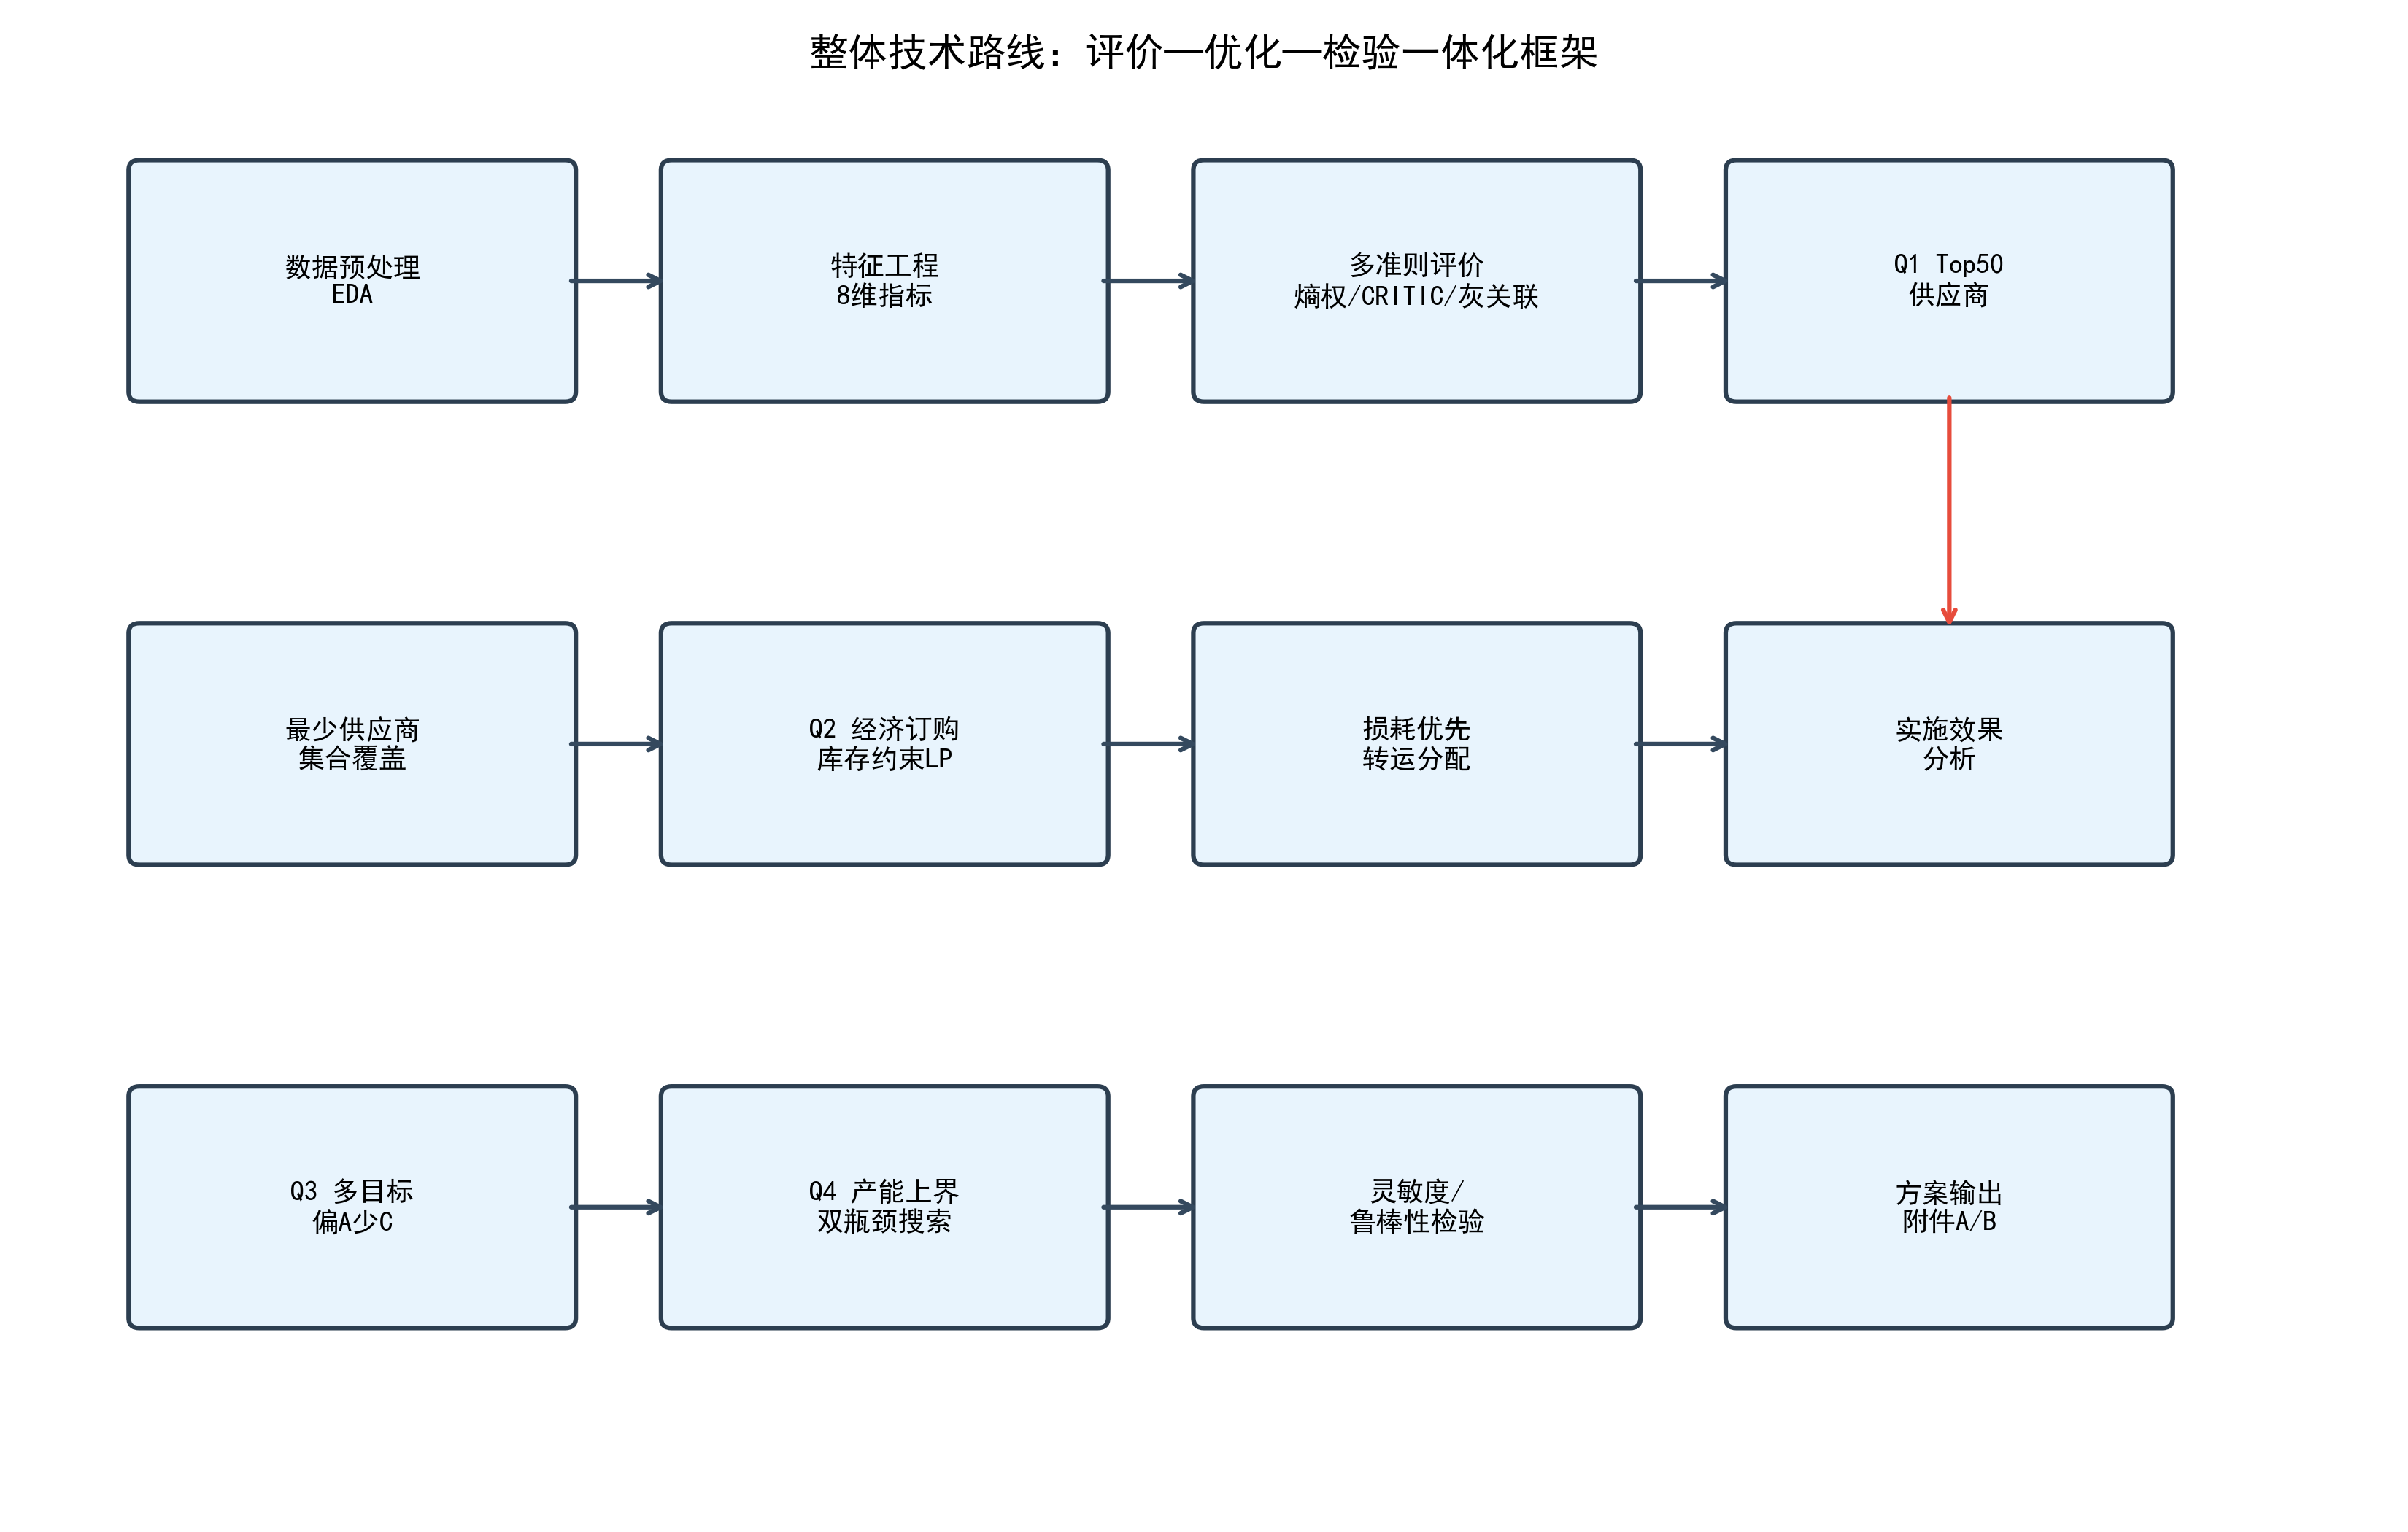
\includegraphics[width=0.95\textwidth]{../output/figures/flowchart_overall.png}
\caption{整体技术路线：评价—优化—检验一体化框架}
\label{fig:flow}
\end{figure}


\section{模型假设与符号说明}

\subsection{基本假设}
\begin{enumerate}[leftmargin=2em,itemsep=0.2em]
\item 未来24周产能需求按当前周产能（或问题4中给定的提升产能）确定，不考虑季节性需求突变；
\item 供应商未来履约可用历史供货满足率$\eta_i$的统计特征刻画，并在鲁棒性检验中引入随机扰动；
\item 库存以“产品当量”统一度量，便于A/B/C混用情形下的安全库存约束；
\item 企业全部收购实际供货；订货量决策以预期接收量满足生产与库存为目标；
\item 转运商周运力恒为6000\,m$^3$，损耗率取历史同期或近期统计值；
\item 同一供应商同一周尽量由一家转运商承运；若单周供货超过运力，允许拆分到损耗次优转运商；
\item 采购成本用相对价格指数度量（C类=1），运输与仓储单位费用相同，故体积可作为运仓储成本代理。
\end{enumerate}

\subsection{符号说明}
\begin{table}[H]
\centering
\caption{主要符号说明}
\label{tab:symbol}
\begin{tabular}{clp{7.2cm}}
\toprule
符号 & 单位 & 含义 \\
\midrule
$i\in\mathcal{S}$ & — & 供应商集合，$\lvert\mathcal{S}\rvert=402$ \\
$k\in\mathcal{T}$ & — & 转运商集合，$\lvert\mathcal{T}\rvert=8$ \\
$t=1,\ldots,T$ & 周 & 计划期，$T=24$；历史期$T_h=240$ \\
$m(i)\in\{A,B,C\}$ & — & 供应商$i$材料类型 \\
$Q_{it},S_{it}$ & m$^3$ & 订货量、供货量 \\
$\eta_i$ & — & 供应商$i$历史平均满足率 \\
$e_m$ & m$^3$/m$^3$ & 材料$m$单位产品消耗系数 \\
$p_m$ & — & 材料$m$相对采购价格 \\
$C_0,\lambda$ & m$^3$,— & 基准周产能与产能倍增系数 \\
$I_t$ & m$^3$ & 第$t$周末库存（产品当量） \\
$L_{kt}$ & \% & 转运商$k$第$t$周损耗率 \\
$X_{ikt}$ & m$^3$ & 供应商$i$经转运商$k$在第$t$周转运量 \\
$U$ & m$^3$/周 & 单转运商运力上限，$U=6000$ \\
$w_j,C_i$ & — & 第$j$指标熵权与TOPSIS贴近度 \\
\bottomrule
\end{tabular}
\end{table}

\section{数据预处理与探索性分析}

对附件1订货矩阵$\mathbf{O}\in\mathbb{R}^{402\times240}$与供货矩阵$\mathbf{S}$，缺失按0处理。定义供应商$i$的活跃周集合$\mathcal{A}_i=\{t:S_{it}>0\}$。清洗后保存至\texttt{data/processed/}。EDA显示：三类供应商数量分布不均；累计供货呈右偏；满足率与周均供货存在弱—中等相关；转运商平均损耗差异显著。这些事实支持“多指标综合评价”而非单一规模排序。

\begin{figure}[H]
\centering
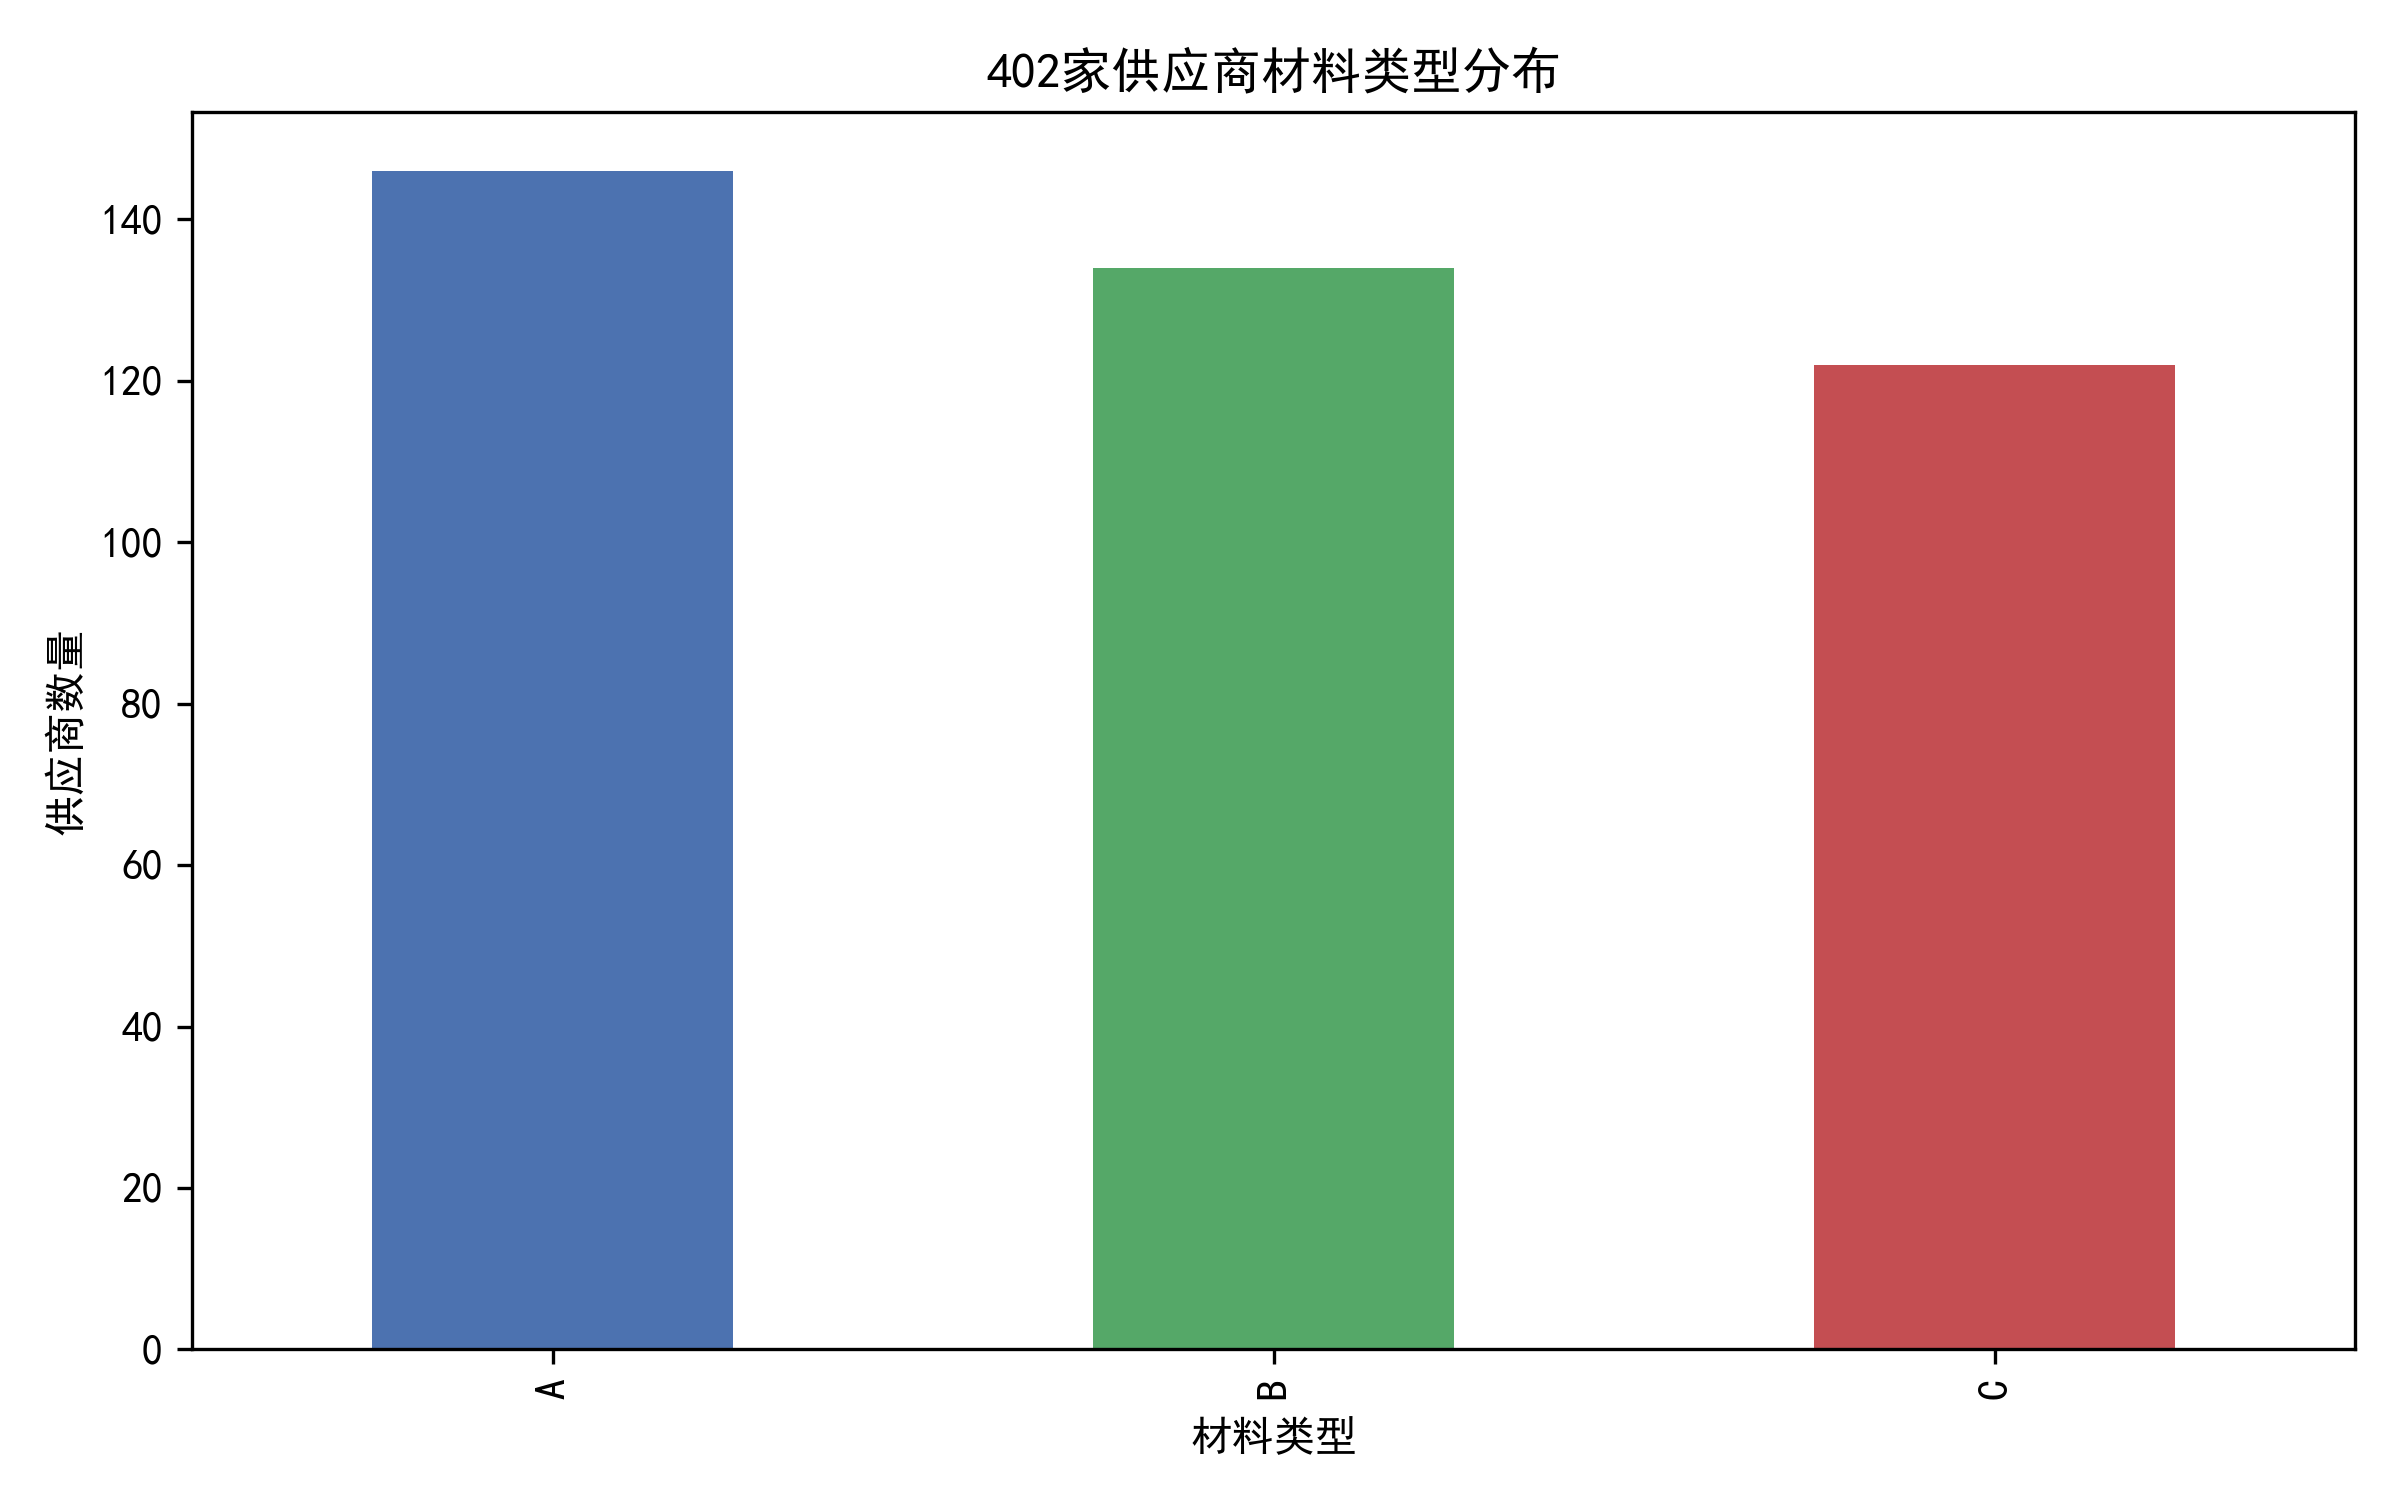
\includegraphics[width=0.72\textwidth]{../output/figures/eda_material_distribution.png}
\caption{402家供应商材料类型分布}
\label{fig:matdist}
\end{figure}

\begin{figure}[H]
\centering
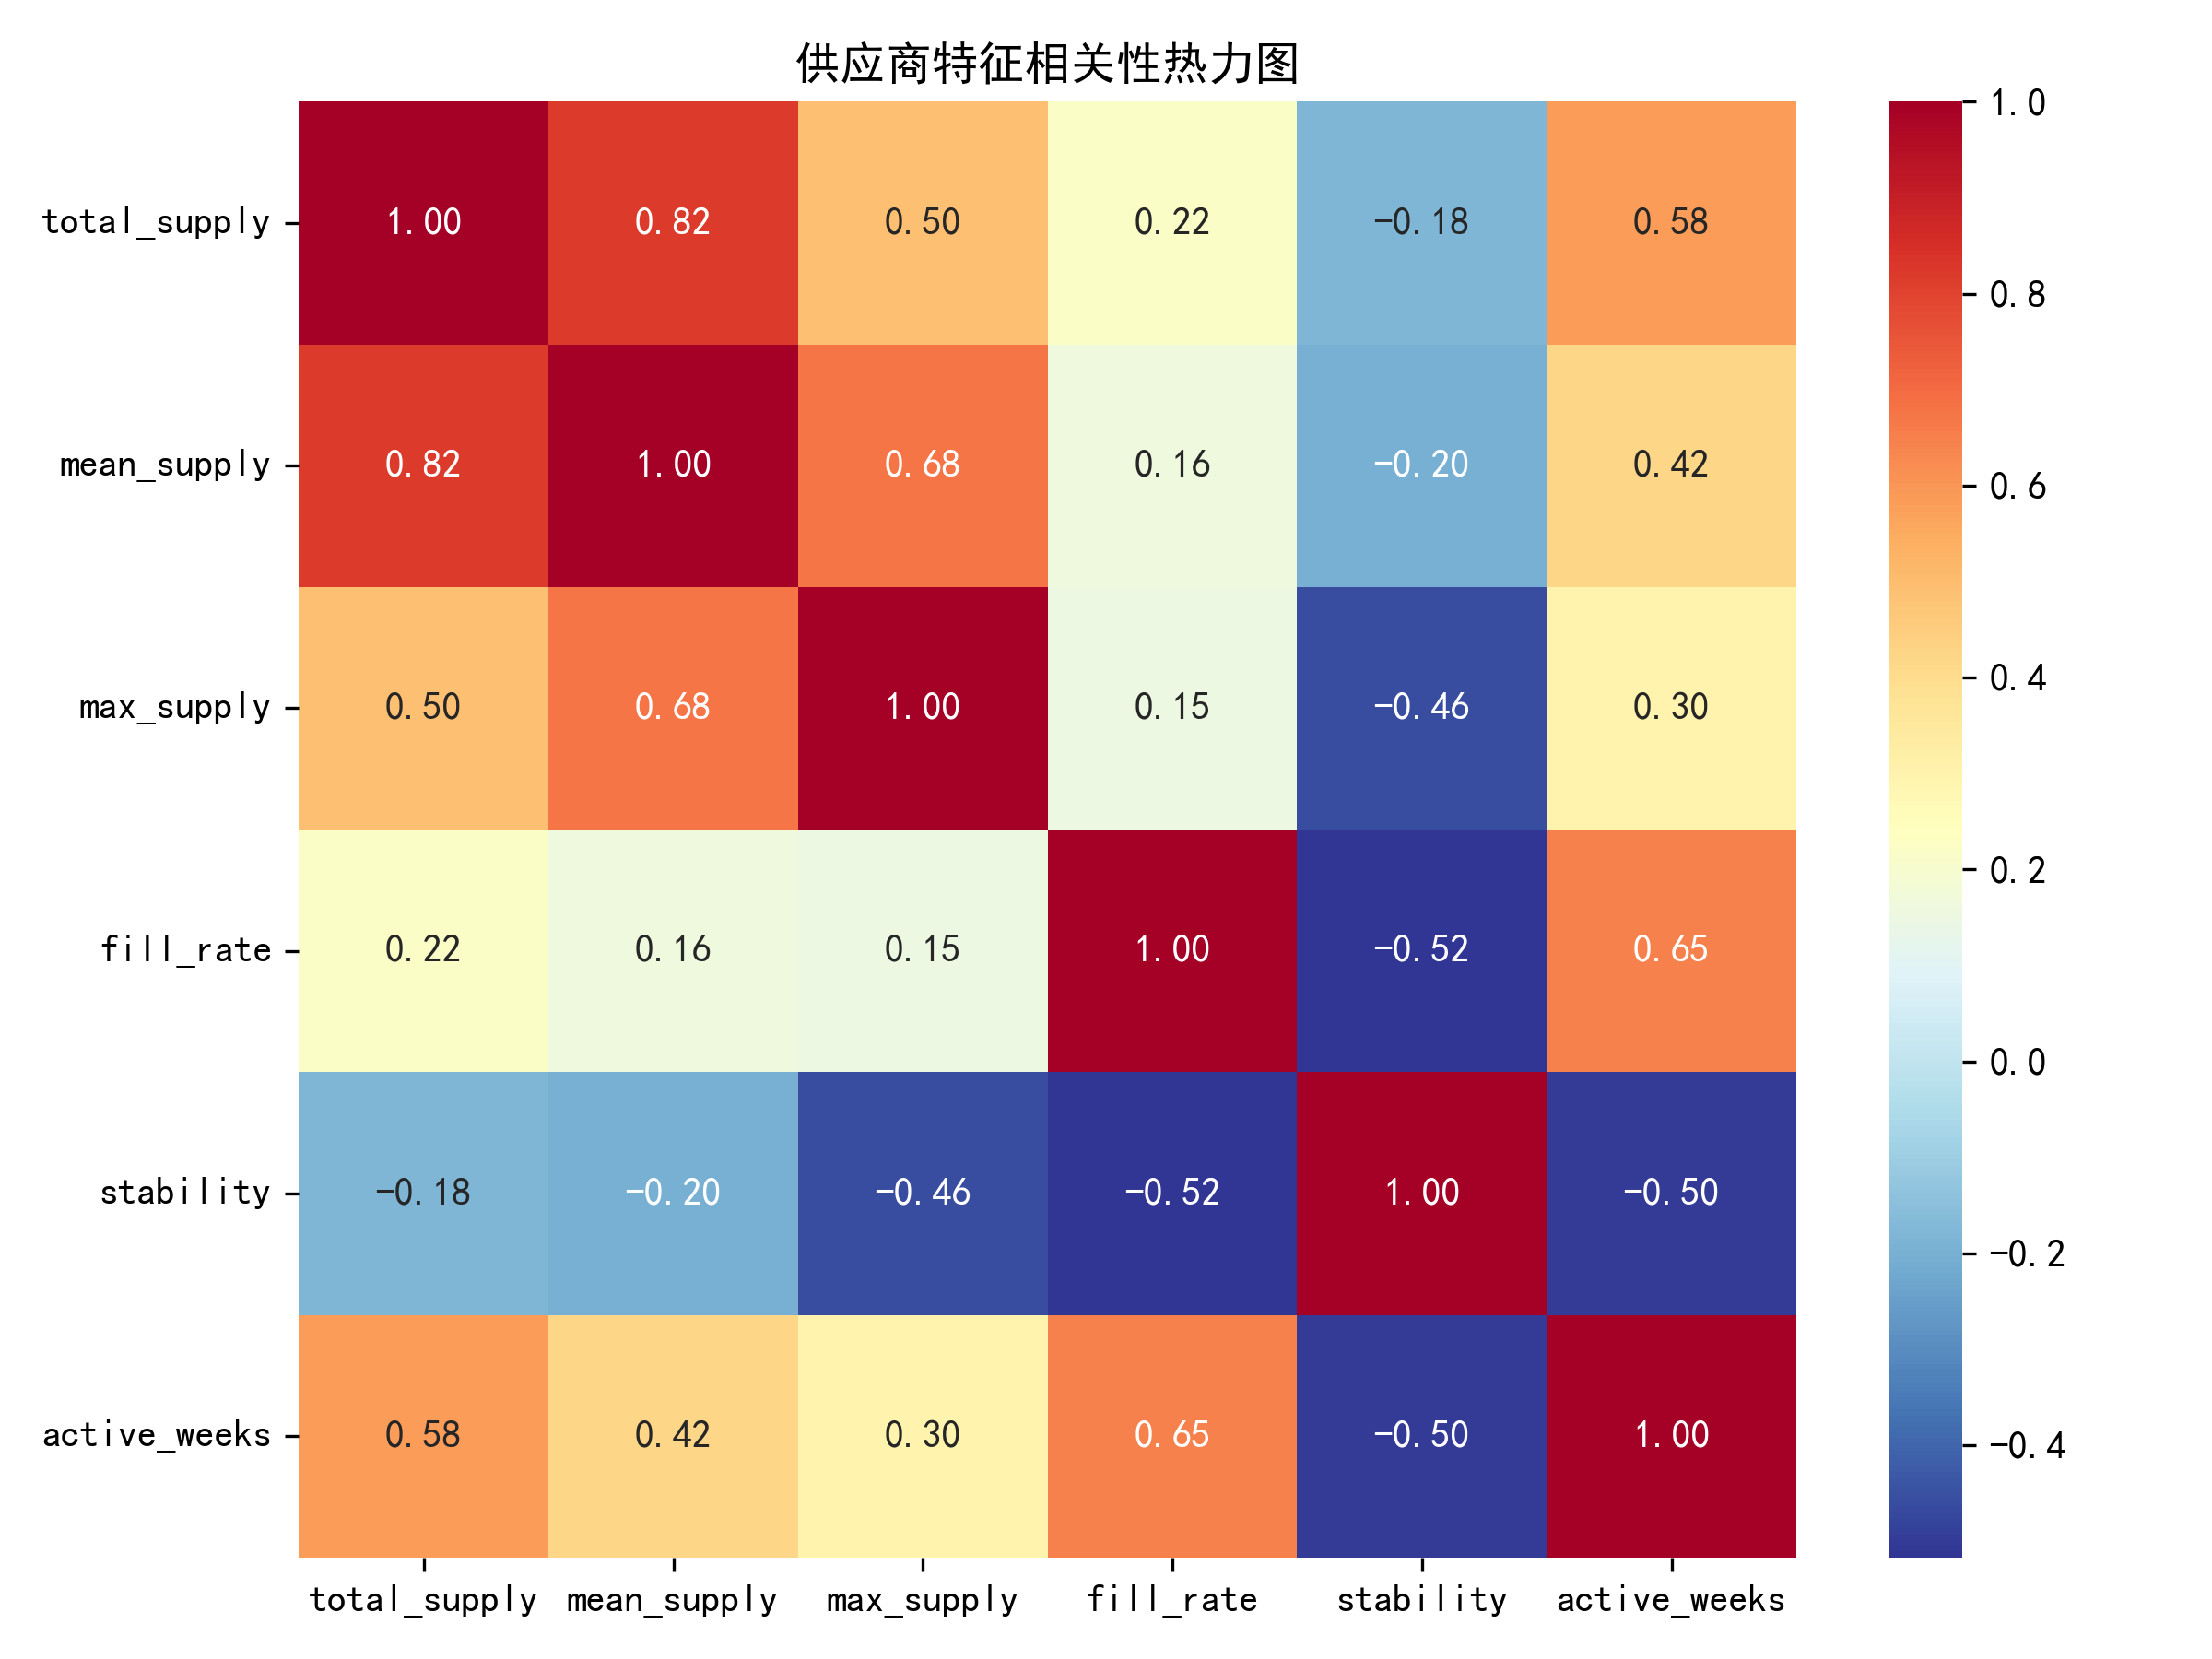
\includegraphics[width=0.78\textwidth]{../output/figures/eda_correlation_heatmap.png}
\caption{供应商特征相关性热力图}
\label{fig:corr}
\end{figure}

\begin{figure}[H]
\centering
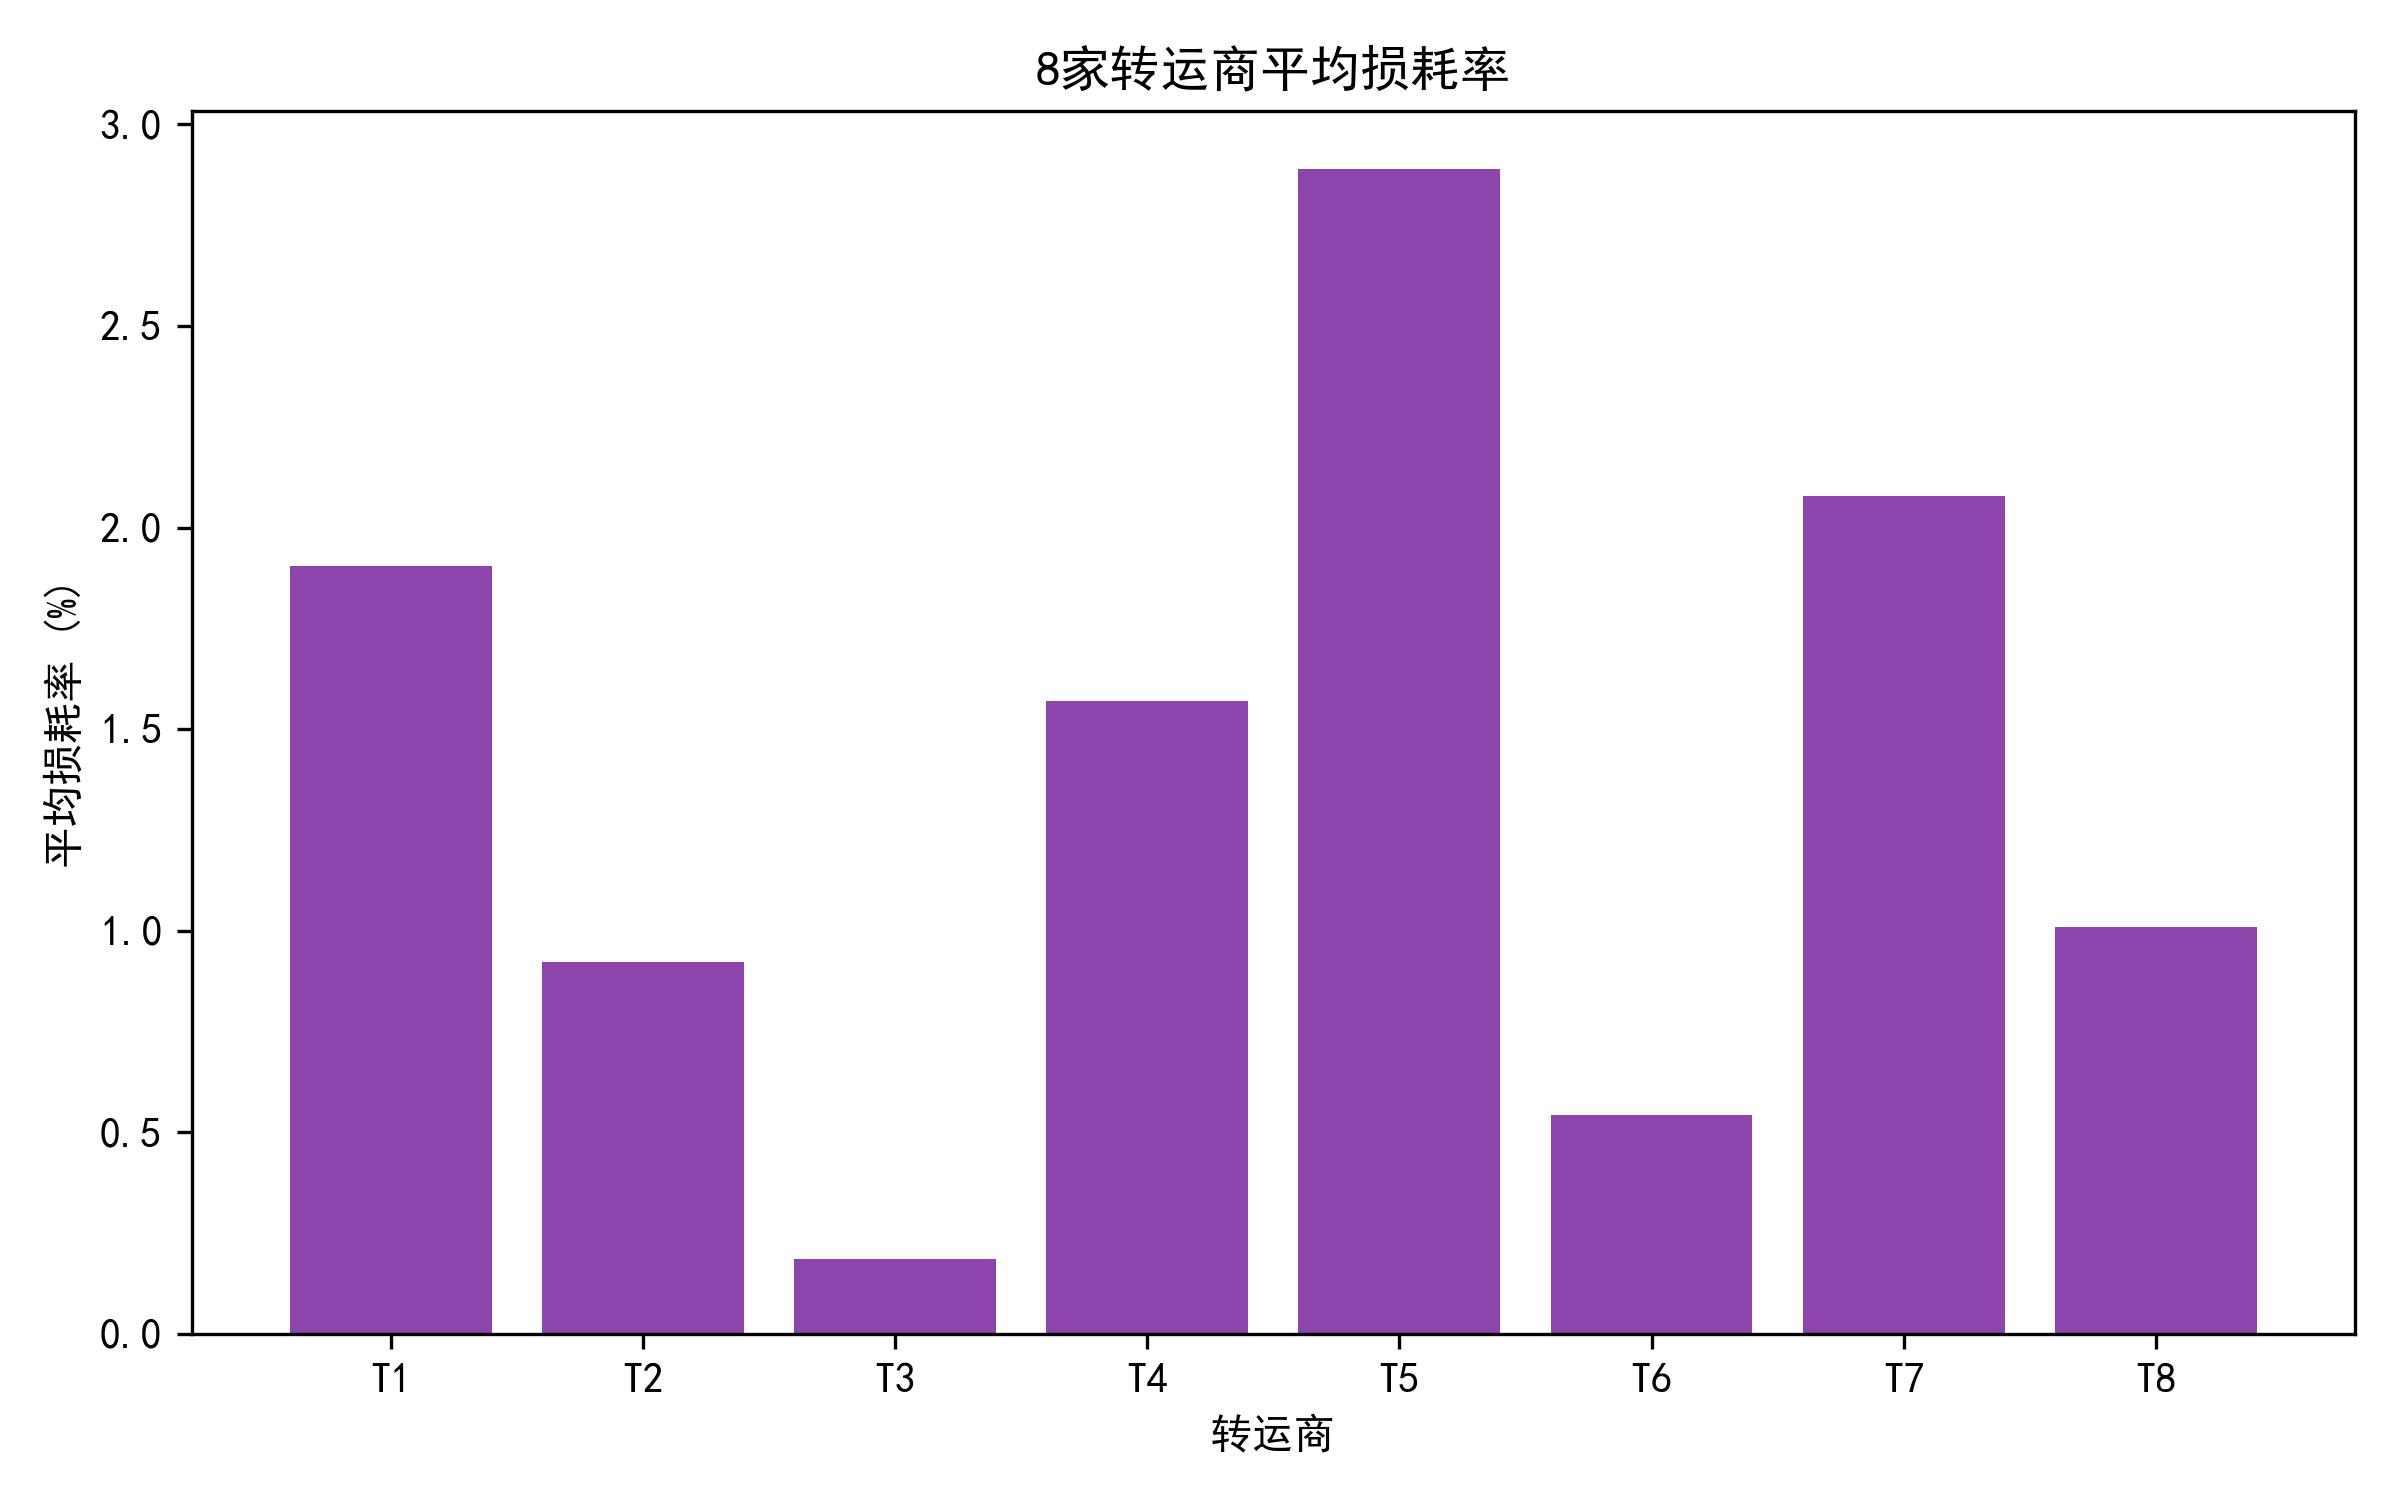
\includegraphics[width=0.72\textwidth]{../output/figures/eda_transporter_loss.png}
\caption{8家转运商历史平均损耗率}
\label{fig:tloss}
\end{figure}


\section{问题一：供应商重要性评价模型}

\subsection{重要性内涵与指标构造}
“保障企业生产的重要性”应同时体现：（1）\textbf{可供规模}——能否提供足够原材料；（2）\textbf{履约可靠}——订货后实际供货是否充分；（3）\textbf{过程稳定}——供货波动是否可控；（4）\textbf{近期能力}——近24周是否仍活跃。据此构造指标向量$\mathbf{x}_i=(x_{i1},\ldots,x_{i8})$：
\begin{align}
x_{i1}&=\sum_{t=1}^{T_h}S_{it},\quad
x_{i2}=\frac{x_{i1}}{\lvert\mathcal{A}_i\rvert+\varepsilon},\quad
x_{i3}=\max_t S_{it},\\
x_{i4}&=\eta_i=\mathrm{mean}_{t:O_{it}>0}\frac{S_{it}}{O_{it}},\\
x_{i5}&=\frac{1}{1+\mathrm{CV}_i},\quad
\mathrm{CV}_i=\frac{\mathrm{std}(S_{i\cdot})}{x_{i2}+\varepsilon},\\
x_{i6}&=\lvert\mathcal{A}_i\rvert,\quad
x_{i7}=\sum_{t=T_h-23}^{T_h}S_{it},\quad
x_{i8}=\phi(m(i)),
\end{align}
其中$\phi(A)=\phi(C)=1,\phi(B)=0.95$用于轻微刻画材料差异（A消耗更低，C单价更低）。全部指标均为效益型。

\subsection{主模型：熵权-TOPSIS}
对决策矩阵$X=(x_{ij})$先极差平移$x_{ij}'=x_{ij}-\min_i x_{ij}+\varepsilon$，再列归一
\begin{equation}
p_{ij}=\frac{x_{ij}'}{\sum_{i}x_{ij}'}.
\end{equation}
第$j$指标熵与差异系数、权重为
\begin{align}
E_j&=-\frac{1}{\ln n}\sum_{i=1}^{n}p_{ij}\ln(p_{ij}+\varepsilon),\quad
d_j=1-E_j,\\
w_j&=\frac{d_j}{\sum_{\ell=1}^{8}d_\ell}.
\end{align}
TOPSIS标准化与加权矩阵：
\begin{equation}
z_{ij}=\frac{x_{ij}}{\sqrt{\sum_i x_{ij}^2}},\quad
v_{ij}=w_j z_{ij}.
\end{equation}
正负理想解$v_j^+$、$v_j^-$取各列最大/最小（效益型），贴近度
\begin{equation}
\label{eq:topsis}
D_i^\pm=\sqrt{\sum_j(v_{ij}-v_j^\pm)^2},\quad
C_i=\frac{D_i^-}{D_i^++D_i^-}.
\end{equation}
按$C_i$降序取前50名为最重要供应商。

\subsection{对照模型与集成}
为避免单一赋权偏差，引入：
\begin{enumerate}[leftmargin=2em]
\item \textbf{CRITIC-TOPSIS}：权重$w_j^{\mathrm{CR}}\propto \sigma_j\sum_{\ell}\bigl(1-\lvert\rho_{j\ell}\rvert\bigr)$，再代入式\eqref{eq:topsis}；
\item \textbf{灰色关联}：以各指标最大值作参考列，计算灰关联度$\gamma_i$；
\item \textbf{主成分评分}：标准化后取第一主成分得分并归一；
\item \textbf{基准法}：仅按累计供货$x_{i1}$排序。
\end{enumerate}
并计算方法间Top50重叠与Kendall秩相关。

\subsection{求解结果}
熵权与CRITIC权重见表\ref{tab:weights}。主模型Top1为S140（B类），$C_i=0.5991$；Top50平均满足率1.041，平均周均供货446.8\,m$^3$。与累计供货基准的Top50重叠为46/50；熵权与CRITIC的Kendall相关为0.705。

\begin{table}[H]
\centering
\caption{Q1指标权重：熵权法与CRITIC}
\label{tab:weights}
\begin{tabular}{lcc}
\toprule
指标 & 熵权 & CRITIC \\
\midrule
累计供货 & 0.2142 & 0.8197 \\
周均供货 & 0.2014 & 0.0049 \\
峰值供货 & 0.2547 & 0.0763 \\
满足率 & 0.0131 & 0.0000 \\
稳定性 & 0.0027 & 0.0000 \\
活跃周 & 0.0470 & 0.0015 \\
近期供货 & 0.2309 & 0.0976 \\
材料 & 0.0359 & 0.0000 \\
\bottomrule
\end{tabular}
\end{table}

\begin{table}[H]
\centering
\caption{Q1最重要供应商（前15名，完整50名见附录）}
\label{tab:top15}
\begin{tabular}{clccrr}
\toprule
排名 & ID & 材料 & 得分 & 累计供货 & 满足率 \\
\midrule
1 & S140 & B & 0.5991 & 302047 & 1.200 \\
2 & S201 & A & 0.5614 & 81989 & 0.536 \\
3 & S374 & C & 0.4963 & 49224 & 1.312 \\
4 & S229 & A & 0.4912 & 354887 & 0.994 \\
5 & S348 & A & 0.4649 & 92421 & 1.070 \\
6 & S361 & C & 0.4599 & 328080 & 0.992 \\
7 & S151 & C & 0.4335 & 194498 & 0.983 \\
8 & S108 & B & 0.3933 & 240950 & 0.984 \\
9 & S139 & B & 0.3137 & 151862 & 1.244 \\
10 & S340 & B & 0.2800 & 171426 & 0.999 \\
11 & S282 & A & 0.2770 & 169340 & 1.013 \\
12 & S275 & A & 0.2576 & 158553 & 1.003 \\
13 & S126 & C & 0.2483 & 47540 & 0.990 \\
14 & S329 & A & 0.2462 & 156518 & 1.002 \\
15 & S330 & B & 0.2432 & 136652 & 0.986 \\
\bottomrule
\end{tabular}
\end{table}

\begin{figure}[H]
\centering
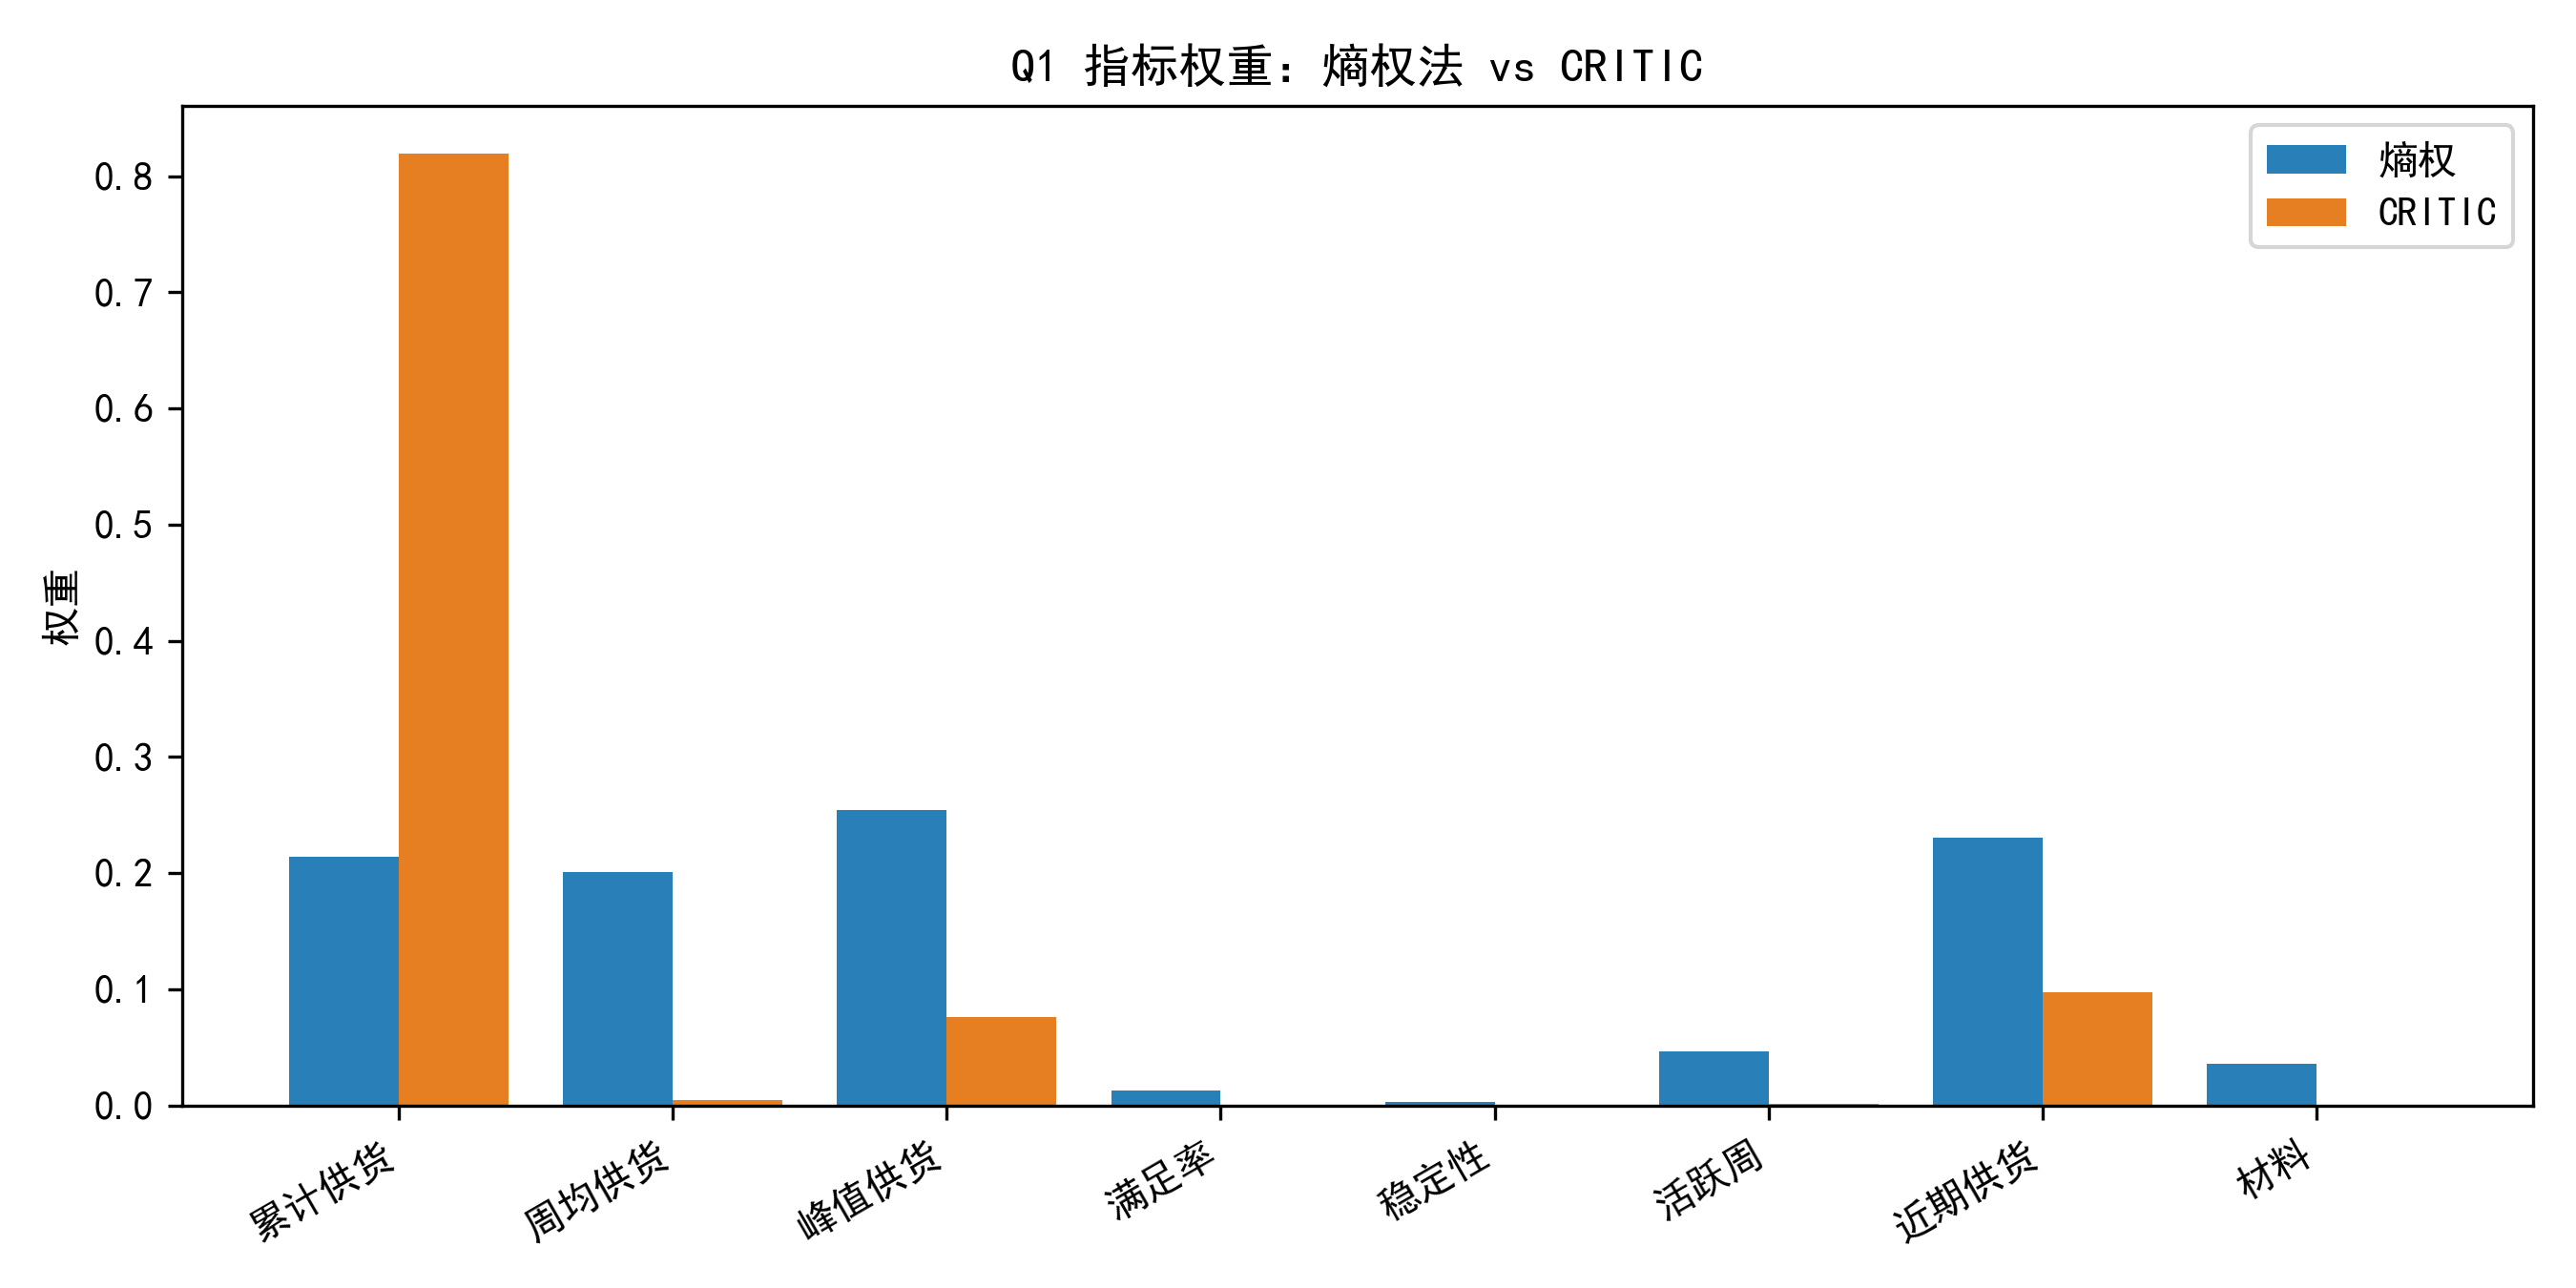
\includegraphics[width=0.85\textwidth]{../output/figures/q1_weight_compare.png}
\caption{熵权与CRITIC权重对比}
\label{fig:wcmp}
\end{figure}

\begin{figure}[H]
\centering
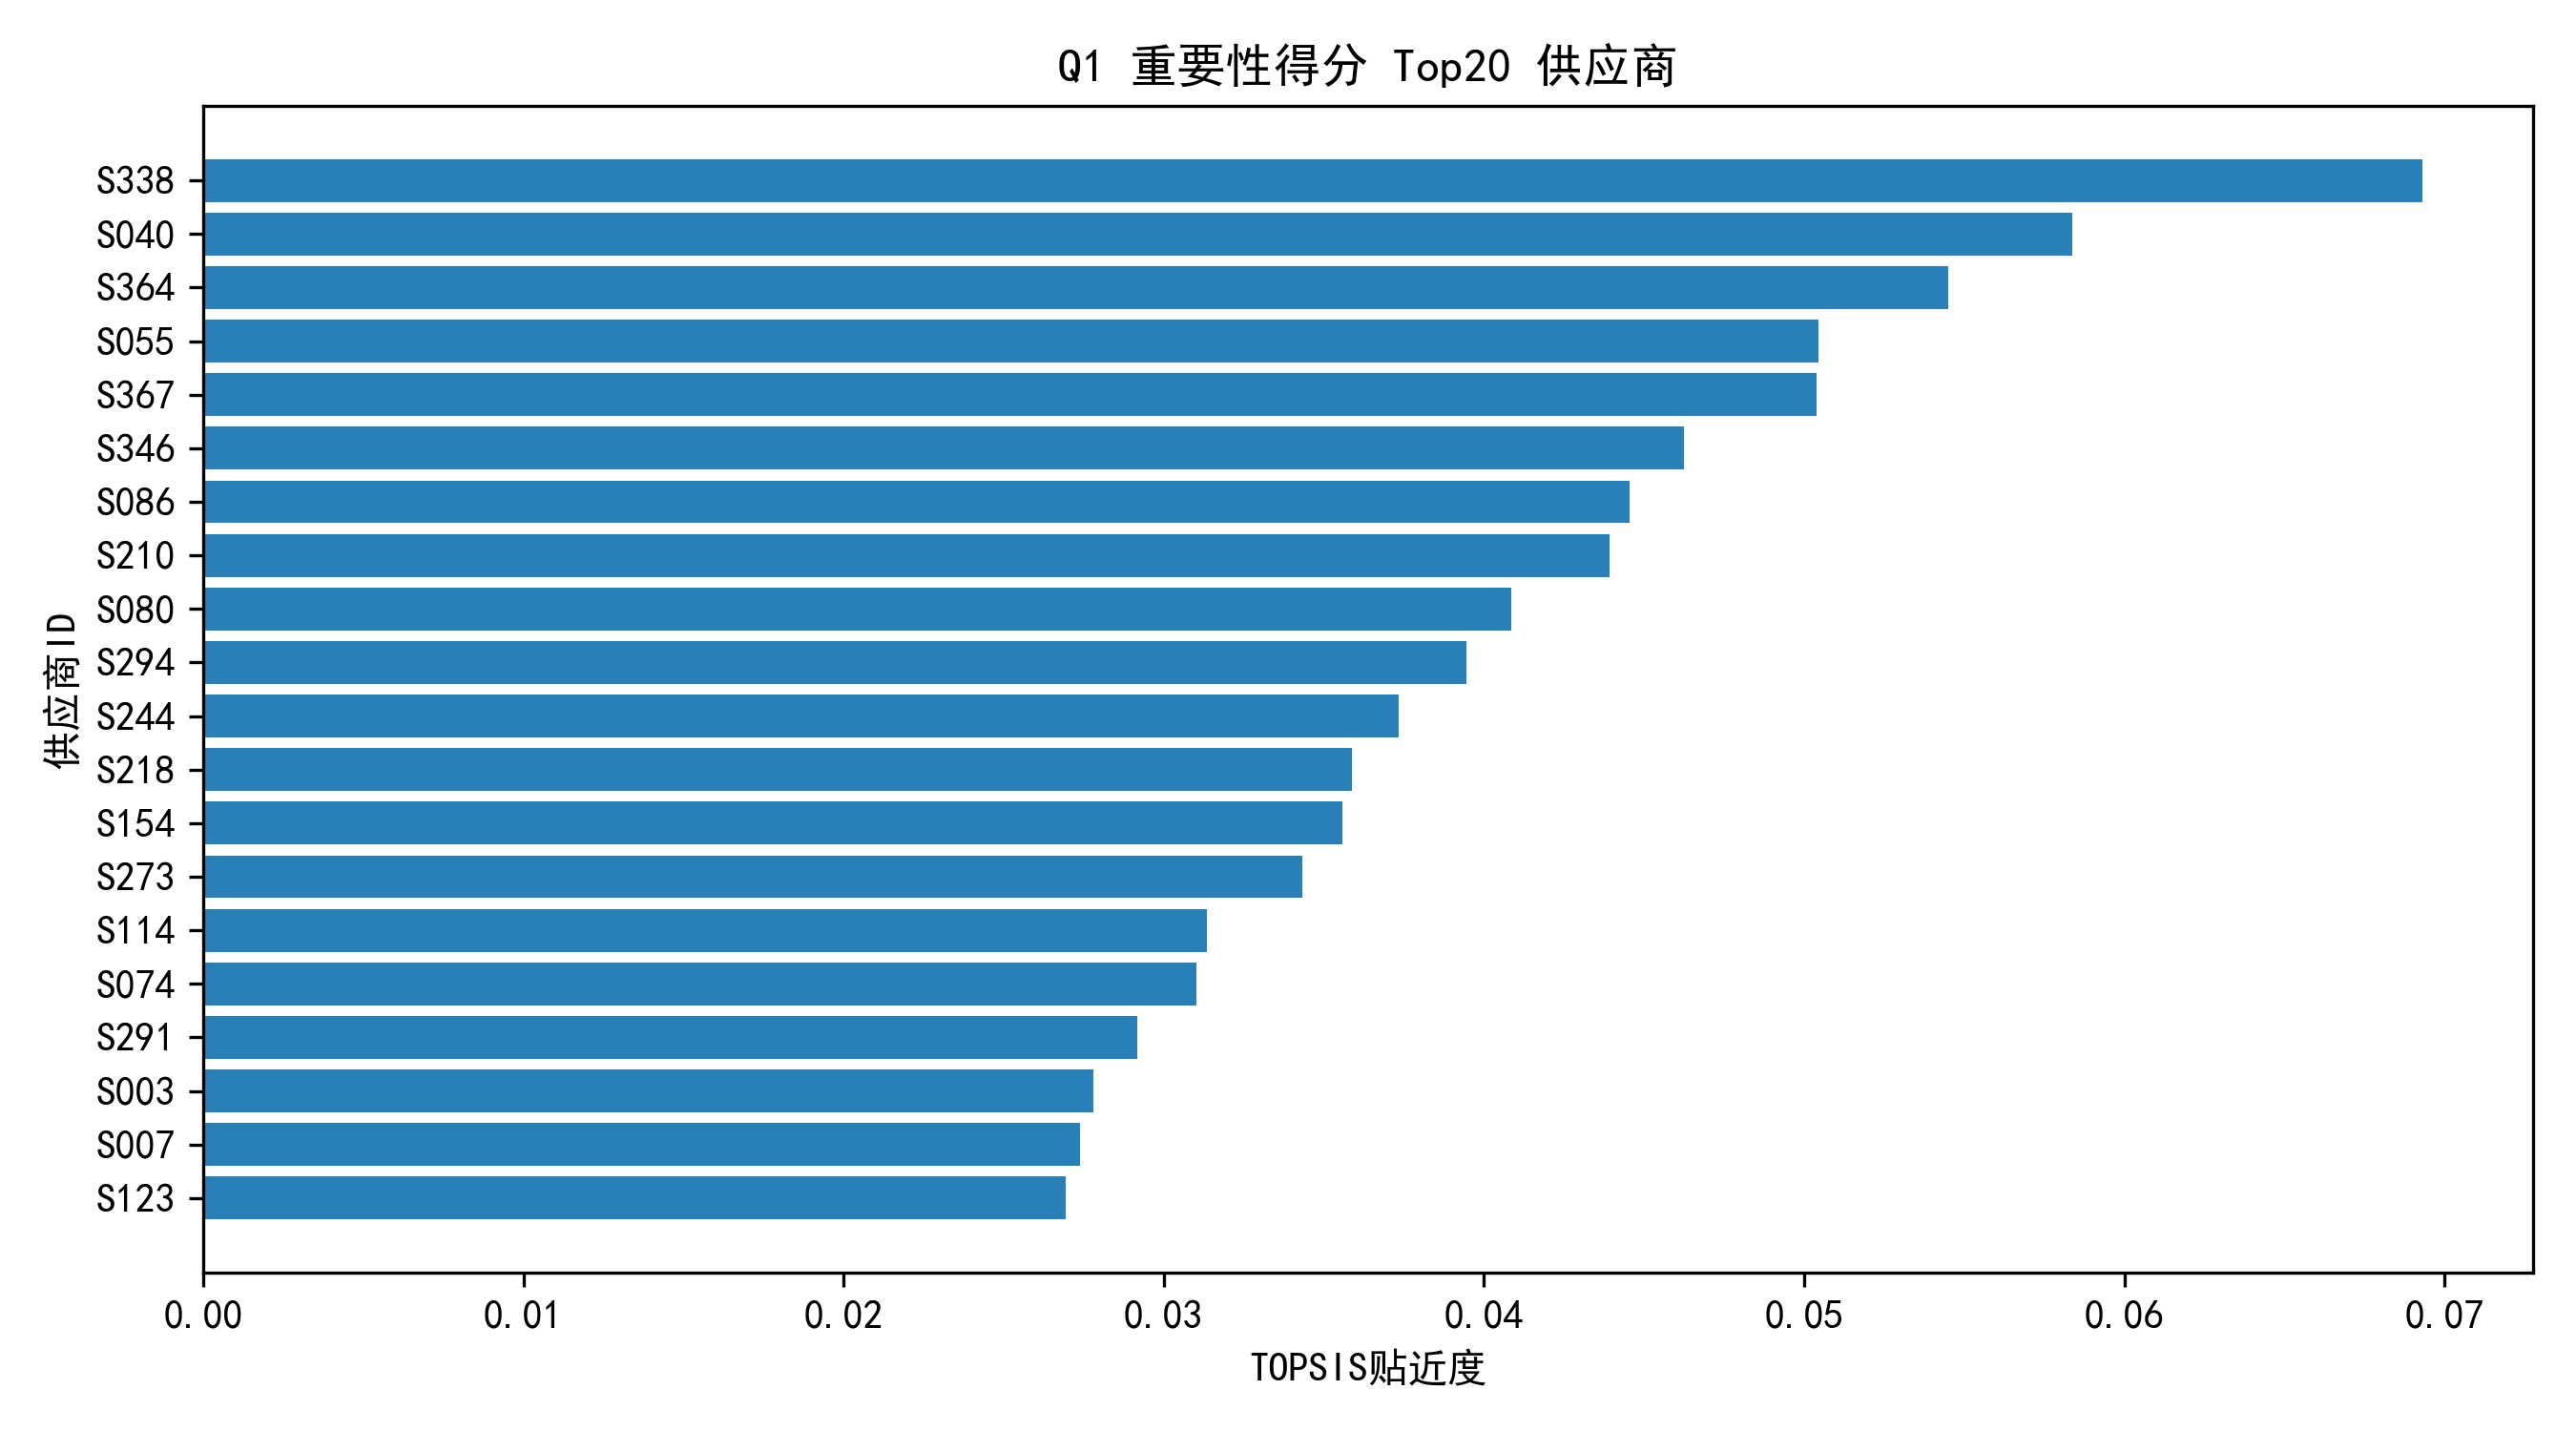
\includegraphics[width=0.82\textwidth]{../output/figures/q1_top20_scores.png}
\caption{重要性得分Top20}
\label{fig:top20}
\end{figure}

\begin{figure}[H]
\centering
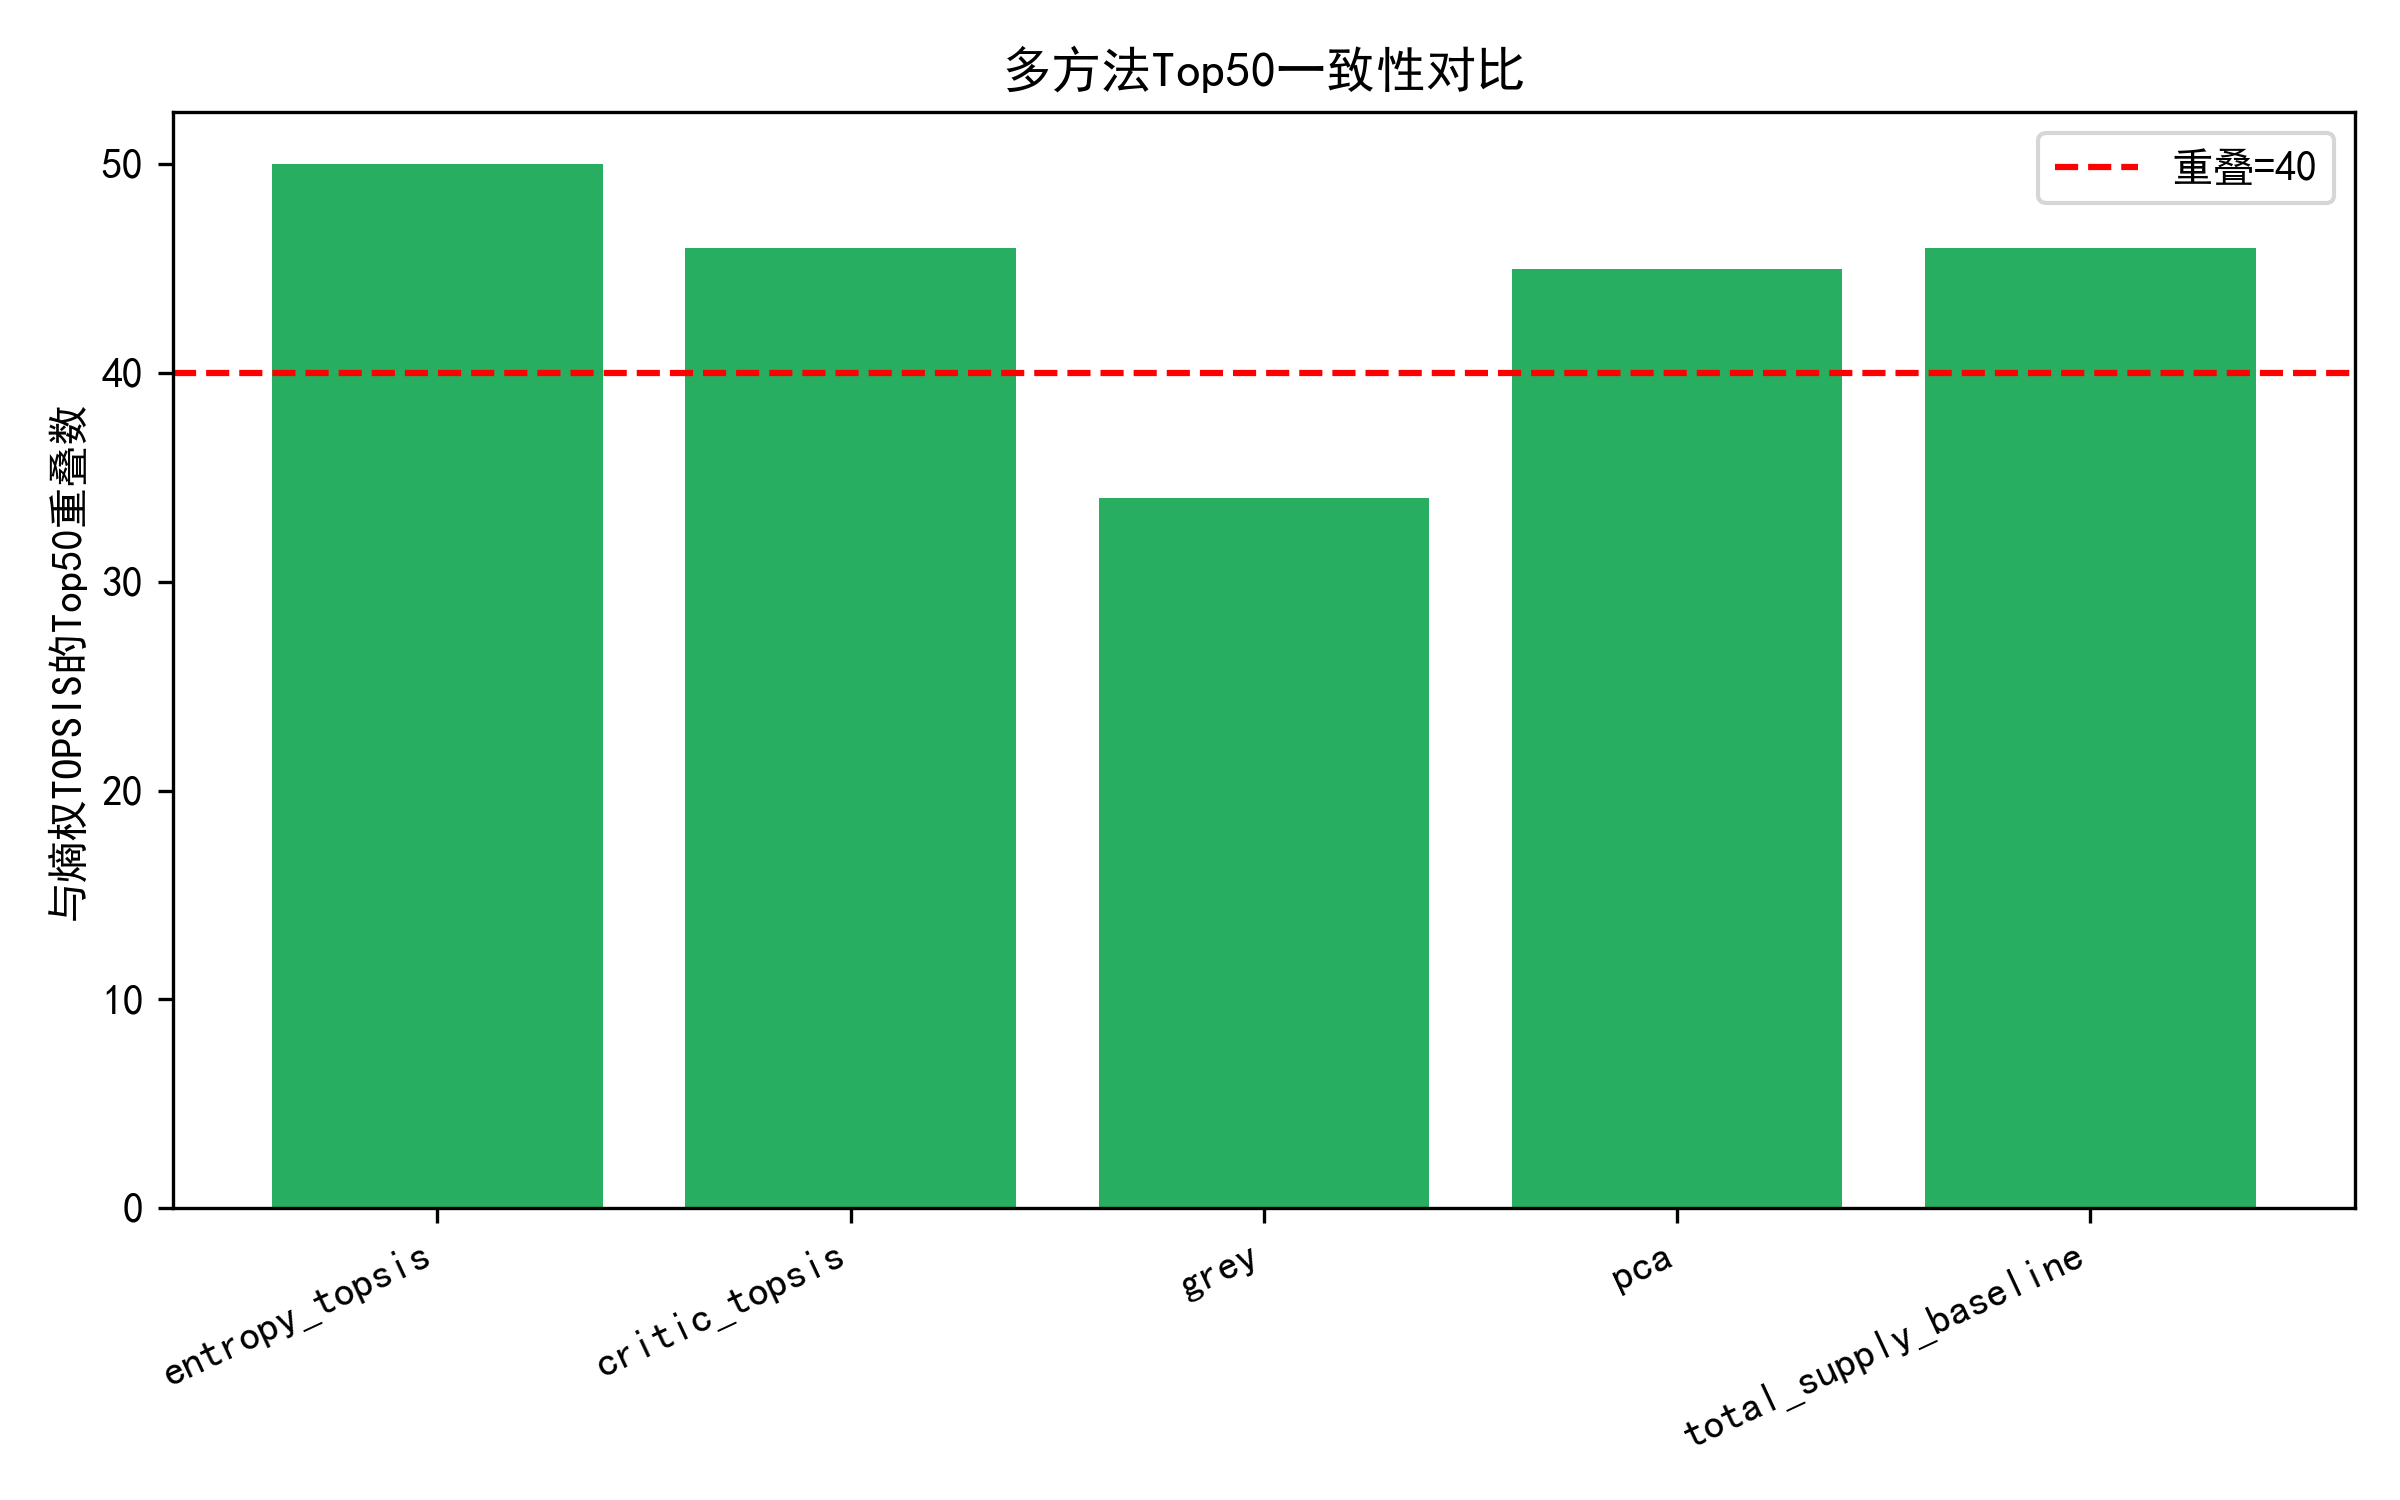
\includegraphics[width=0.82\textwidth]{../output/figures/q1_method_overlap.png}
\caption{多方法Top50重叠对比}
\label{fig:overlap}
\end{figure}


\begin{table}[H]
\centering
\caption{多方法与基准的Top50一致性}
\label{tab:agree}
\begin{tabular}{lcc}
\toprule
方法 & 与熵权TOPSIS重叠 & Jaccard \\
\midrule
entropy\_topsis & 50 & 1.000 \\
critic\_topsis & 46 & 0.852 \\
grey & 34 & 0.515 \\
pca & 45 & 0.818 \\
total\_supply\_baseline & 46 & 0.852 \\
\bottomrule
\end{tabular}
\end{table}

\subsection{问题一小结}
熵权-TOPSIS在保留规模信息的同时显著提升对满足率与稳定性的区分能力；多方法交叉验证表明核心供应商集合高度一致，为问题二“最少供应商筛选”提供可靠先验。

\section{问题二：最少供应商、经济订购与低损耗转运}

\subsection{最少供应商的集合覆盖模型}
记供应商周供货能力估计
\begin{equation}
\hat{a}_i=\min\{x_{i3},\,1.5\,x_{i2}\}.
\end{equation}
在“偏经济”设定下，优先以A类满足产能，周原材料需求近似$R=C_0e_A$。引入安全系数$\beta=1.15$，最少供应商问题为
\begin{equation}
\label{eq:minset}
\min_{\,y_i\in\{0,1\}}\ \sum_{i\in\mathcal{S}} y_i
\quad\mathrm{s.t.}\quad
\sum_{i} \hat{a}_i y_i \ge \beta R.
\end{equation}
实践中按问题一排序贪心累加能力，直至覆盖$\beta R$，得到最少供应商数$N^*=14$，供应商集合记为$\mathcal{S}_2$。

\subsection{带库存约束的经济订购LP}
决策变量$Q_{it}\ge0$（$i\in\mathcal{S}_2,t=1,\ldots,24$），库存$I_t$（产品当量）。预期接收的产品当量为
\begin{equation}
G_t=\sum_{i\in\mathcal{S}_2}\eta_i Q_{it}\frac{1}{e_{m(i)}}.
\end{equation}
库存递推与安全库存：
\begin{align}
I_0&=2C_0,\\
I_t&=I_{t-1}+G_t-C_0,\quad t=1,\ldots,24,\\
I_t&\ge 2C_0.
\end{align}
供应商周能力与总需求软约束：
\begin{equation}
0\le Q_{it}\le\hat{a}_i,\quad
\sum_i\eta_i Q_{it}\ge 0.95R.
\end{equation}
目标为最小化采购成本指数
\begin{equation}
\label{eq:q2obj}
\min\ \sum_{t=1}^{24}\sum_{i\in\mathcal{S}_2} p_{m(i)} Q_{it}.
\end{equation}
该模型为标准线性规划，可用CBC等求解器全局最优求解。

\subsection{损耗最少的转运分配}
给定订购方案后，对每周供货任务$Q_{it}$，按该周损耗率$L_{kt}$升序选择转运商，在运力$U$内分配：
\begin{algorithm}[H]
\caption{损耗优先的转运贪心分配}
\begin{algorithmic}[1]
\FOR{每个供应商$i$、每周$t$}
\STATE 剩余量$r\leftarrow Q_{it}$；按$L_{kt}$升序排列转运商
\FOR{转运商$k$按序}
\STATE $X_{ikt}\leftarrow\min(r,U)$；$r\leftarrow r-X_{ikt}$
\STATE 若$r=0$则停止
\ENDFOR
\ENDFOR
\end{algorithmic}
\end{algorithm}
周加权平均损耗
\begin{equation}
\bar{L}_t=\frac{\sum_{i,k} X_{ikt} L_{kt}}{\sum_{i,k} X_{ikt}+\varepsilon}
\end{equation}
用于实施效果评价。相对“随机指派/平均损耗指派”基线，损耗优先策略可系统性降低高损耗周的暴露。

\subsection{求解结果与实施效果}
最少供应商数$N^*=14$；24周总订货量454271\,m$^3$，成本指数510596。产品当量结构：A\,50.3\%，B\,29.2\%，C\,20.5\%。周订货量稳定覆盖需求线，转运利用率热力图显示高峰周接近运力上界，说明运力约束真实起作用。

\begin{figure}[H]
\centering
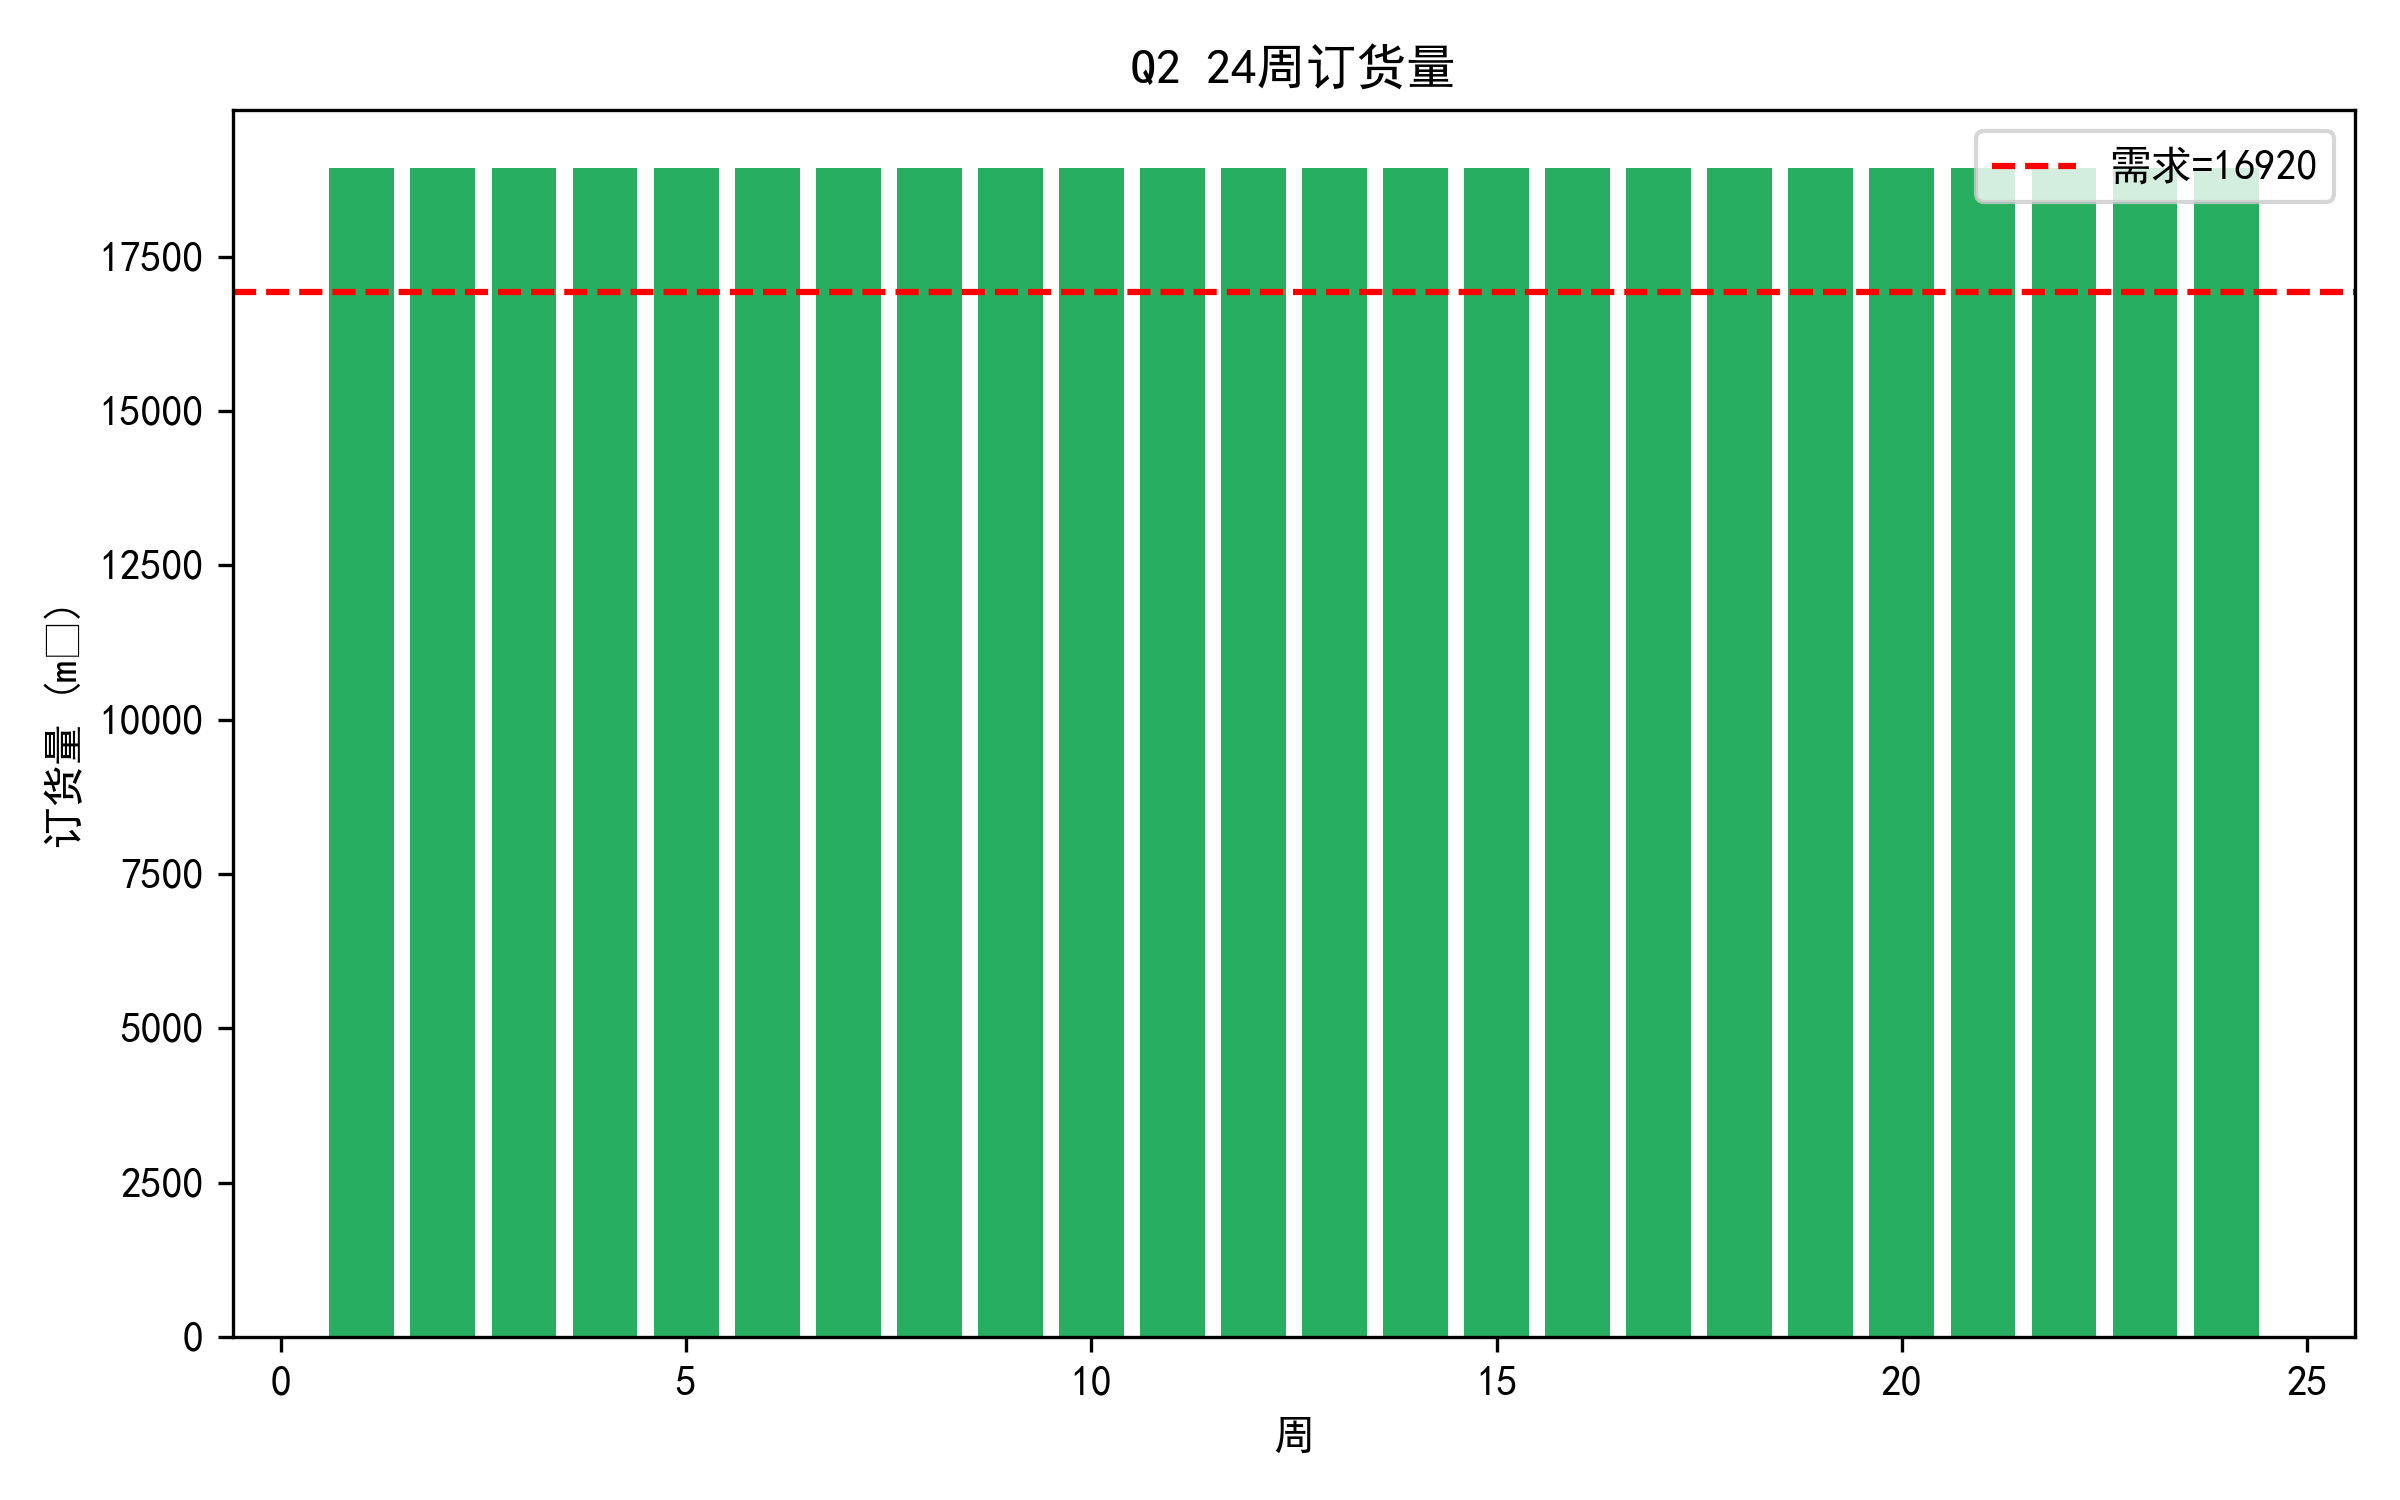
\includegraphics[width=0.78\textwidth]{../output/figures/q2_weekly_orders.png}
\caption{Q2未来24周订货量及需求对照}
\label{fig:q2ord}
\end{figure}

\begin{figure}[H]
\centering
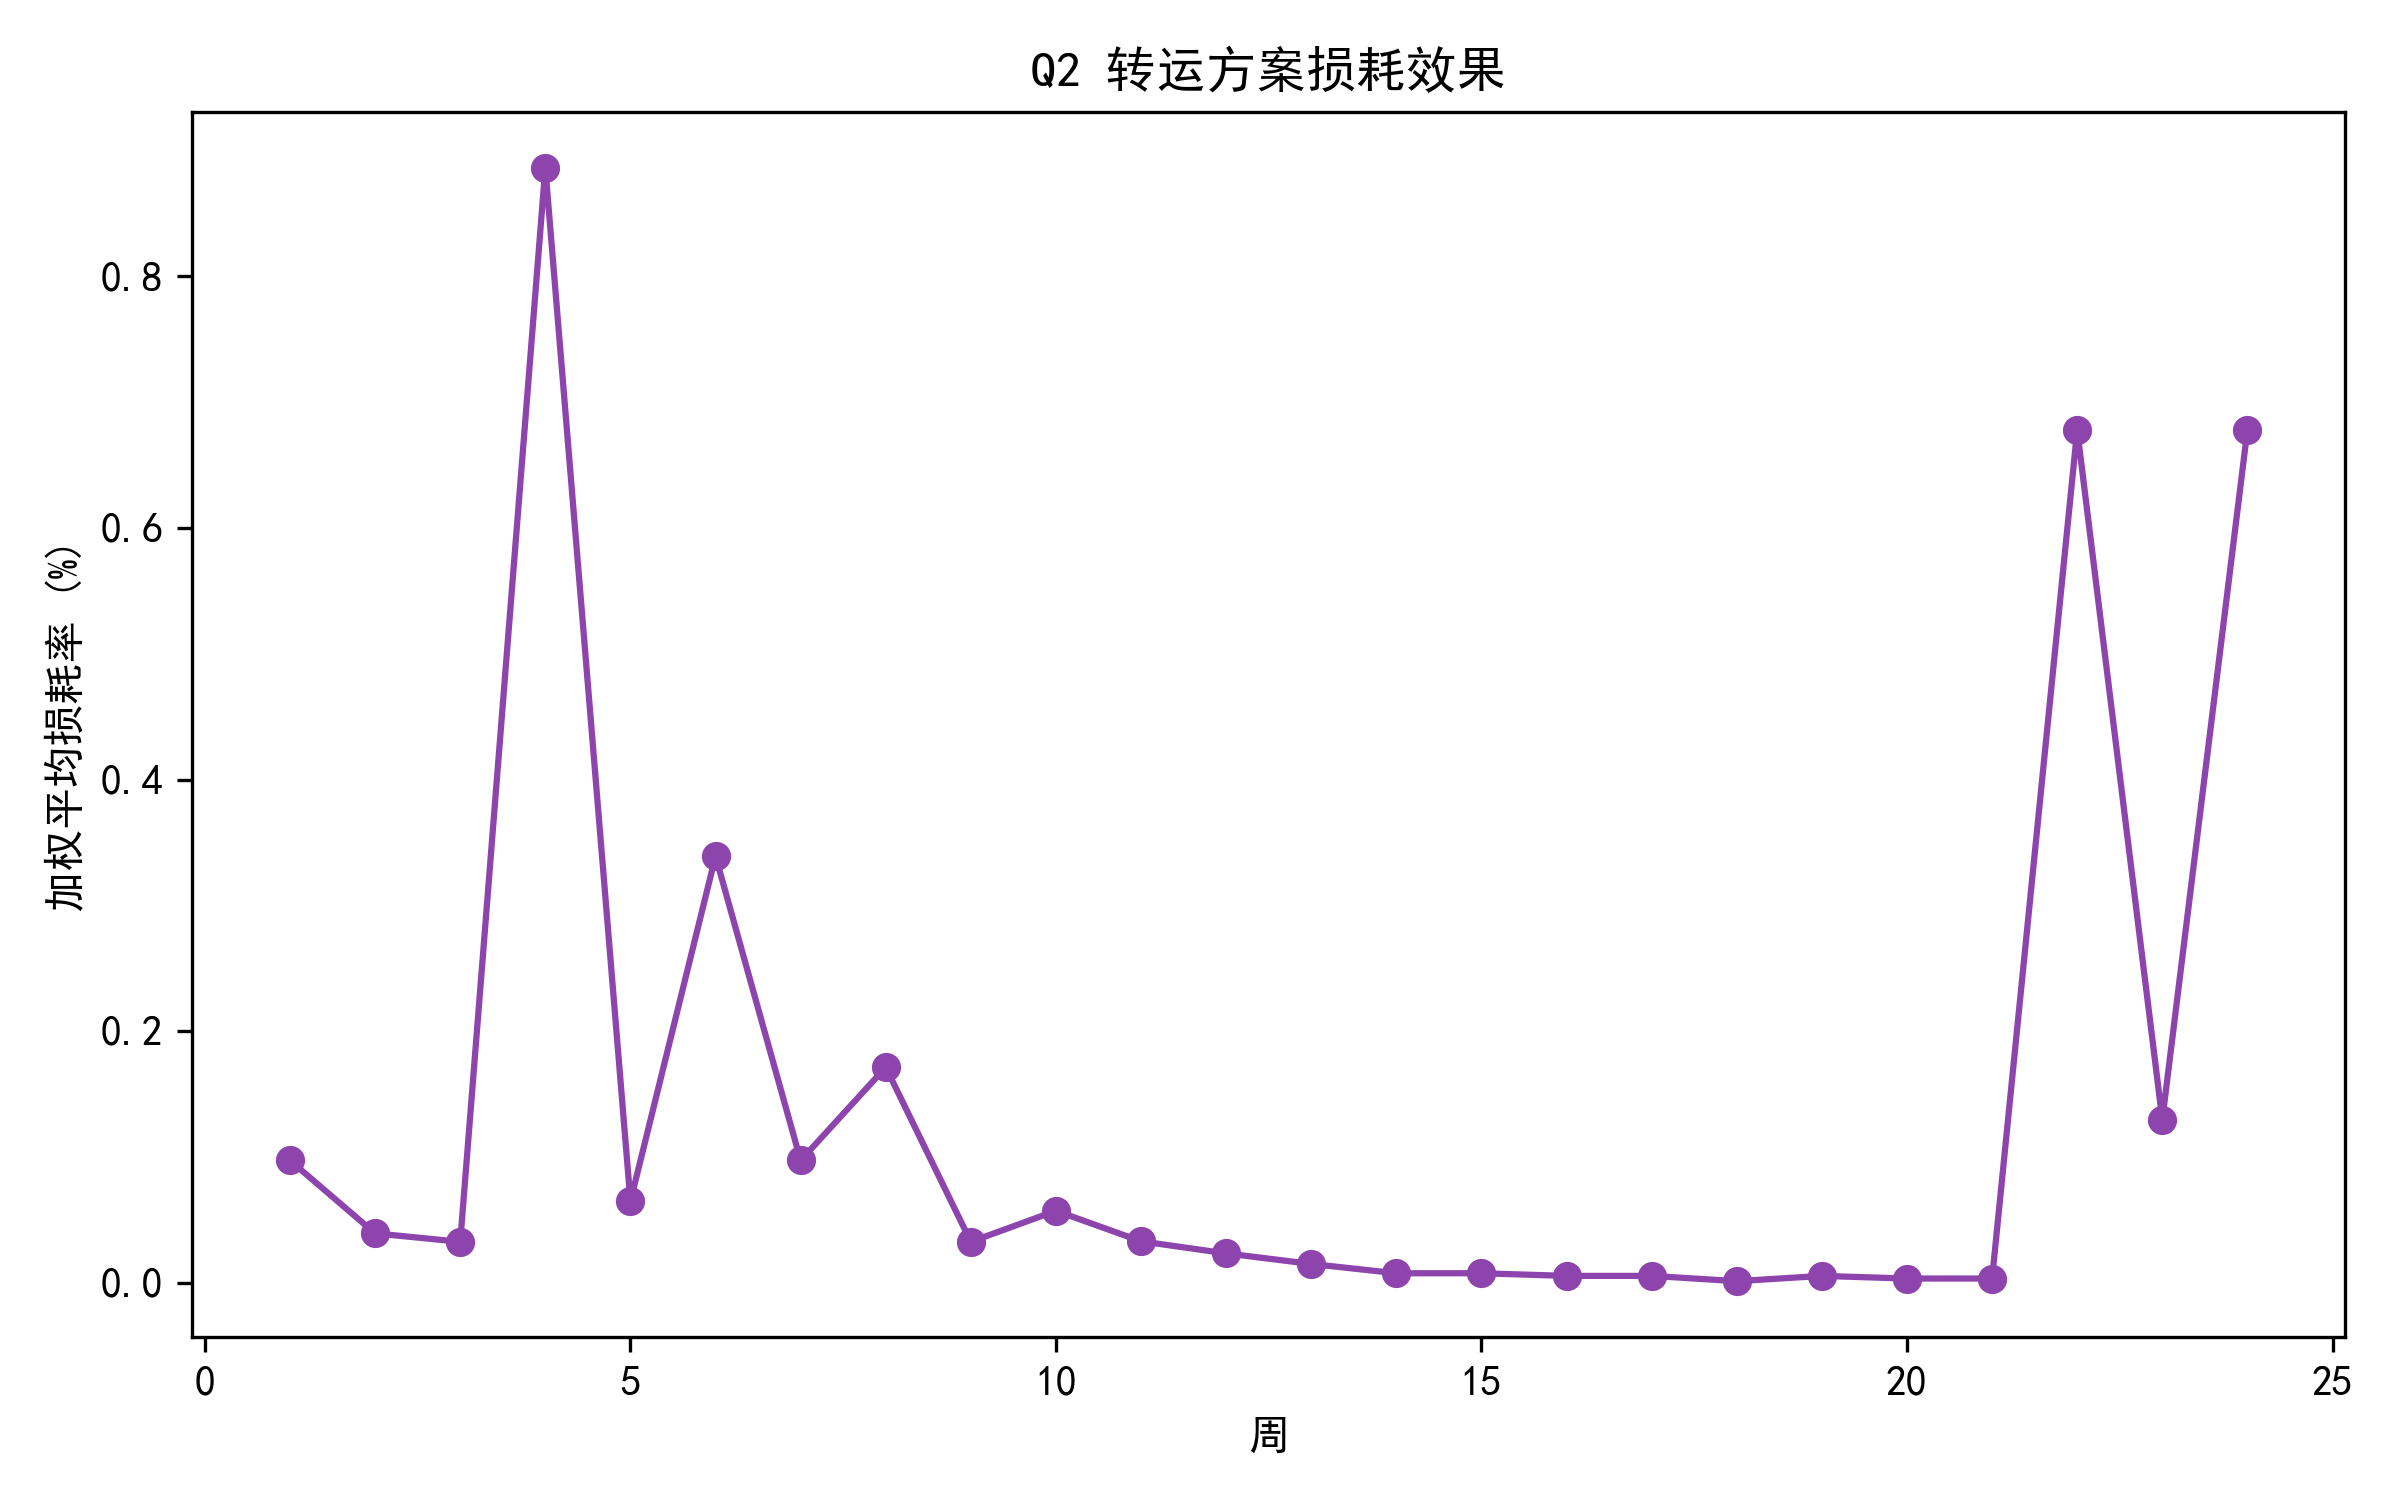
\includegraphics[width=0.78\textwidth]{../output/figures/q2_transport_loss.png}
\caption{Q2转运方案加权损耗率周序列}
\label{fig:q2loss}
\end{figure}

\begin{figure}[H]
\centering
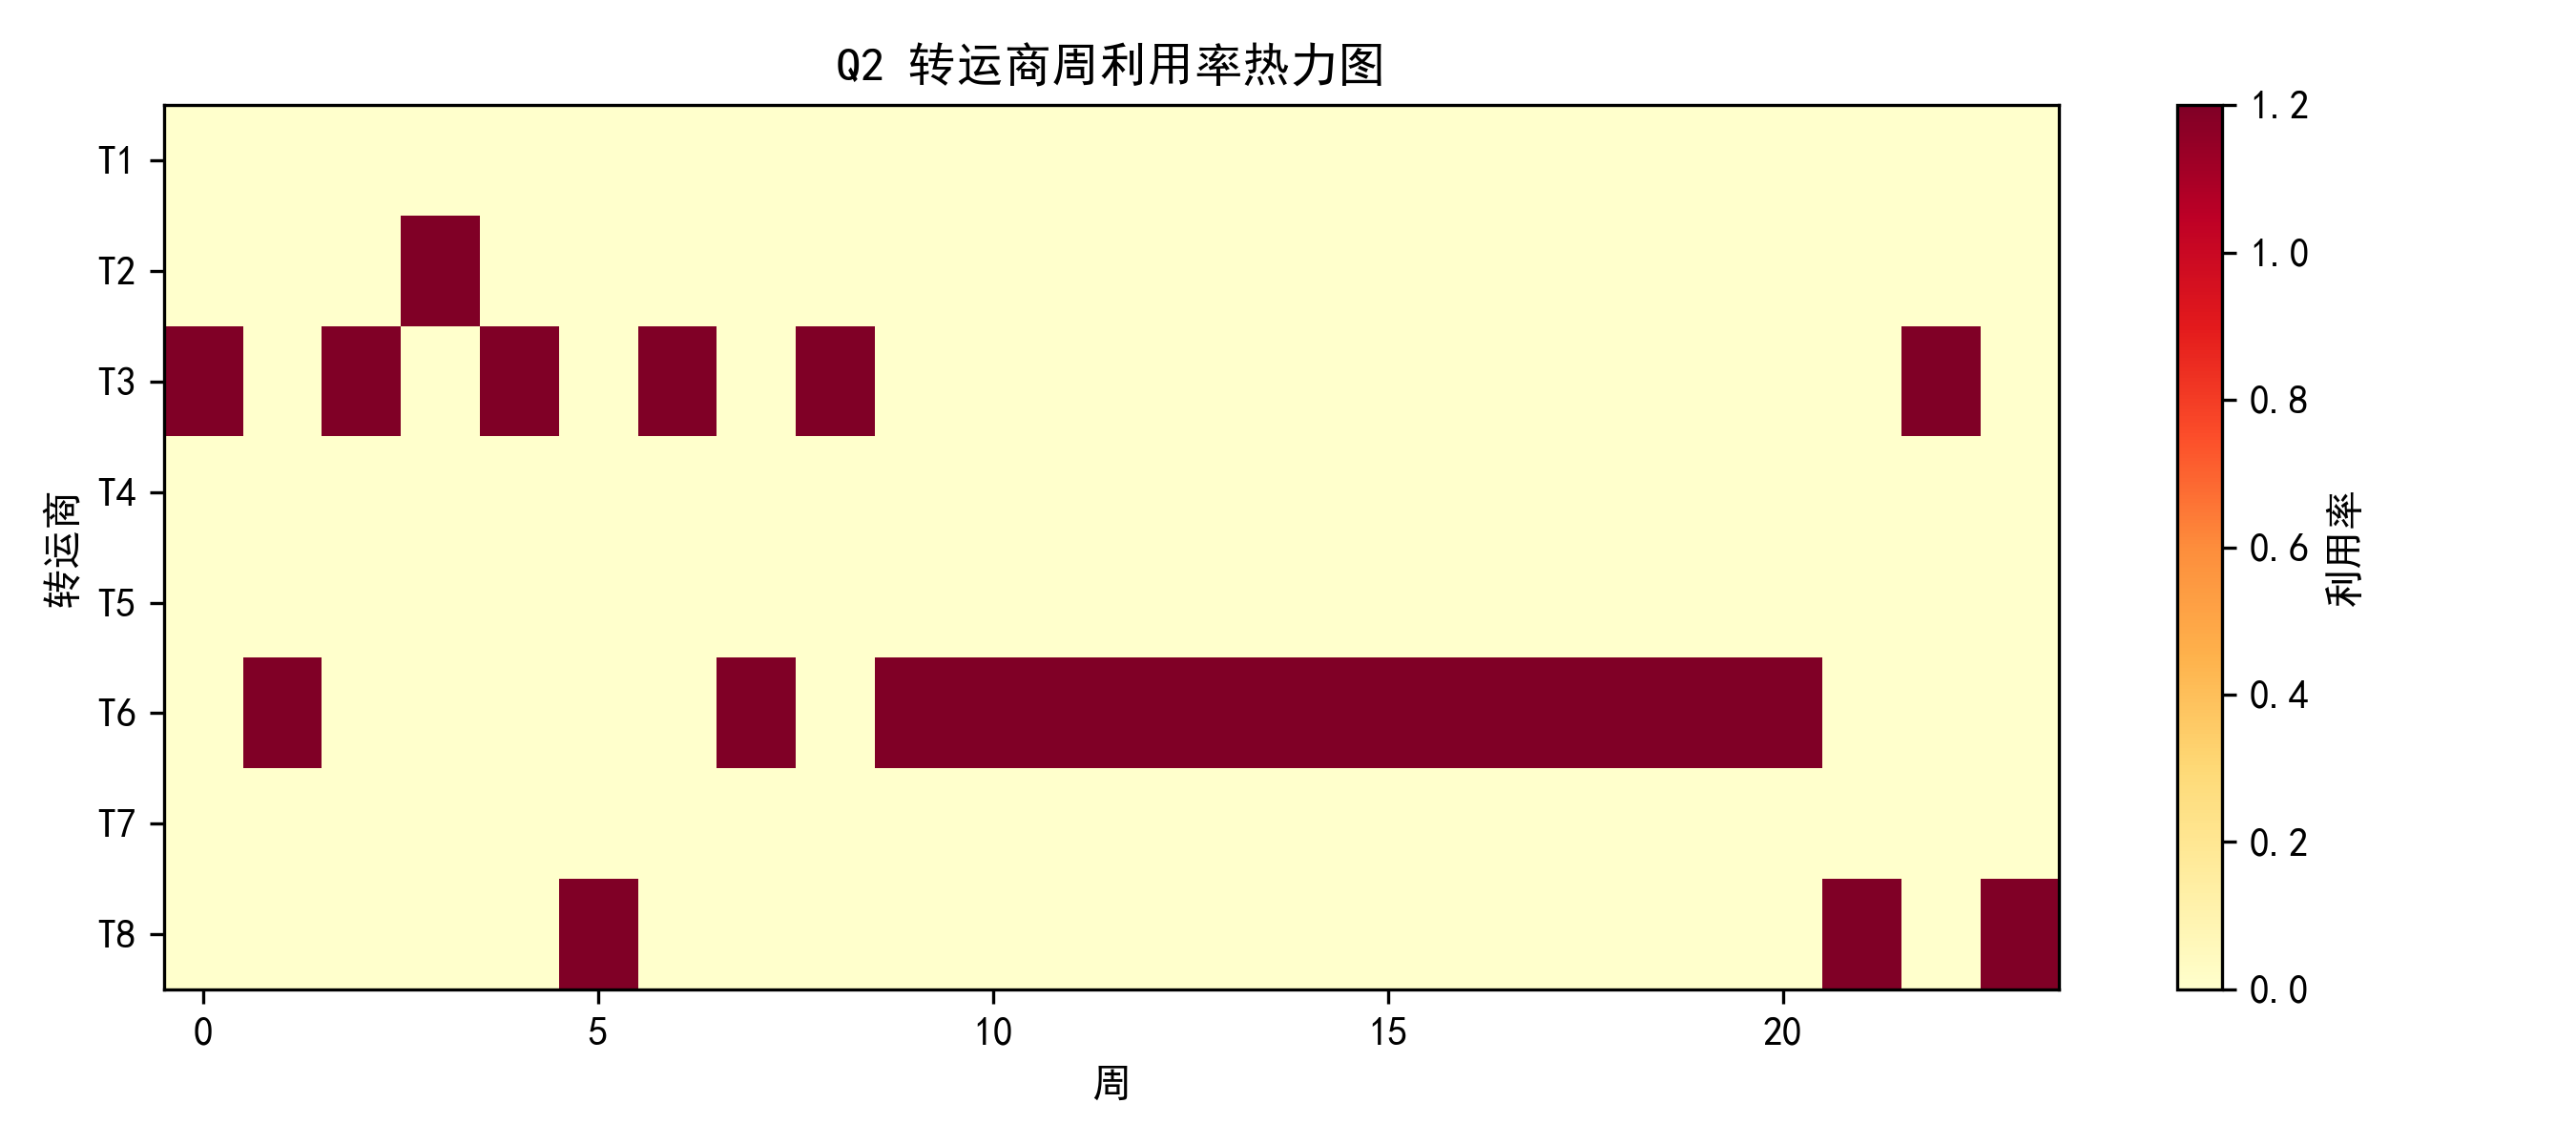
\includegraphics[width=0.88\textwidth]{../output/figures/q2_transport_util_heatmap.png}
\caption{Q2转运商周利用率热力图}
\label{fig:q2util}
\end{figure}

\begin{figure}[H]
\centering
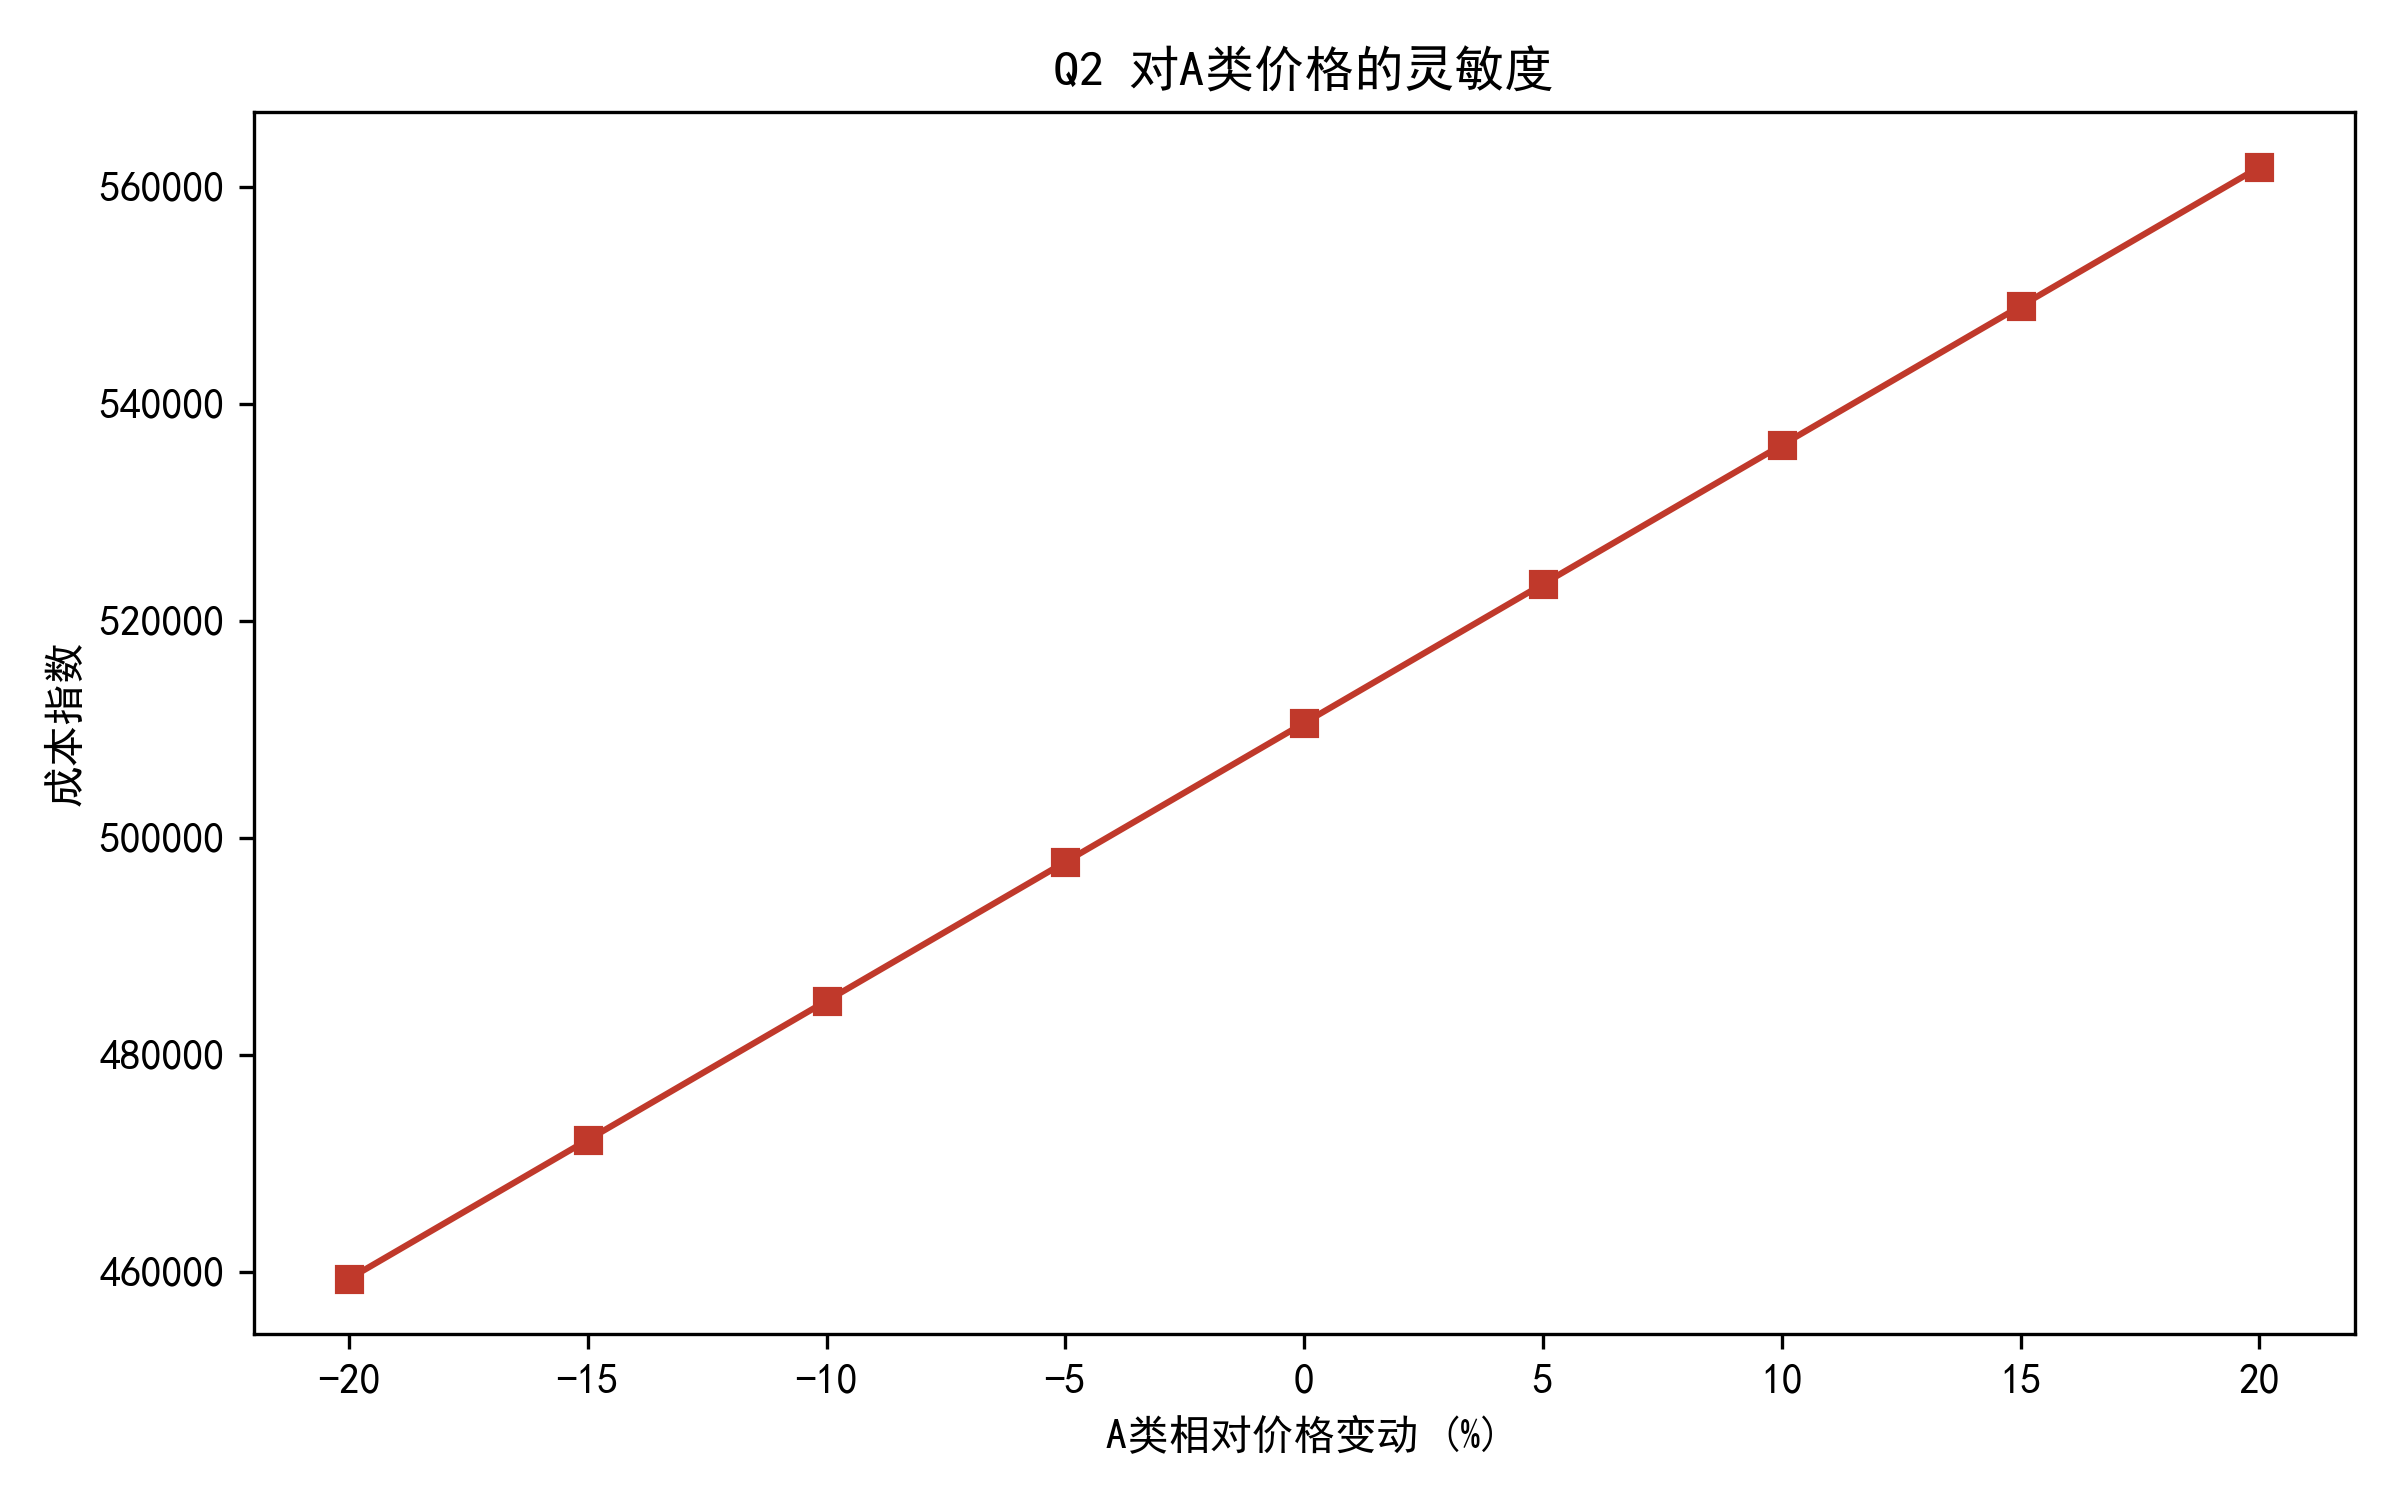
\includegraphics[width=0.78\textwidth]{../output/figures/q2_price_sensitivity.png}
\caption{Q2对A类相对价格变动的成本灵敏度}
\label{fig:q2price}
\end{figure}


\subsection{问题二小结}
在问题一排序指导下，$N^*=14$已能覆盖$\beta R$；LP保证两周安全库存；损耗优先转运降低高损耗暴露。方案已写入附件A/B对应工作表。

\section{问题三：偏A少C的结构优化订购与转运}

\subsection{从问题二到问题三的目标切换}
问题三强调：尽量多采购A、尽量少采购C，以减少转运与仓储体积，并希望损耗更低。注意题目未规定固定配比，故本文将“结构偏好”落实为：
\begin{enumerate}[leftmargin=2em]
\item 供应商筛选层：提高A类优先级、降低C类优先级；
\item 优化层：在库存与产能约束下继续最小化成本指数，但可行供应商集合更偏向A；
\item 评价层：用产品当量份额$\alpha_m=\dfrac{\sum_{i:m(i)=m}\eta_i Q_{it}/e_m}{\sum_i\eta_i Q_{it}/e_{m(i)}}$刻画结构变化。
\end{enumerate}

设供应商调整优先级
\begin{equation}
r_i'=r_i-\Delta_A\mathbf{1}_{m(i)=A}-\Delta_C\mathbf{1}_{m(i)=C},
\end{equation}
其中$\Delta_A>0,\Delta_C<0$，再按$r_i'$重选集合$\mathcal{S}_3$，并求解与式\eqref{eq:q2obj}同型的LP，转运算法不变。

\subsection{为何A类有利于压缩运仓储}
完成单位产品所需原材料体积为$e_m$，故
\begin{equation}
e_A<e_B<e_C\ \Rightarrow\ \text{同等产能下A类原材料体积最小}.
\end{equation}
在运仓储单价相同假设下，提高A份额等价于降低运仓储成本代理指标。C类虽采购单价最低，但体积惩罚最大；问题三明确牺牲部分采购单价优势以换取体积节约。

\subsection{结果与对比分析}
Q3选用28家供应商；总订货407931\,m$^3$（较Q2降10.2\%）；成本指数473854（降7.2\%）。产品当量：A由50.3\%升至63.8\%，C由20.5\%降至0.0\%，B为36.2\%。B上升主因Top供应商（如S140）为B类且能力强，仍保留在集合中——这体现“重要性优先”与“结构偏好”的折中，而非简单剔除一切非A。

\begin{table}[H]
\centering
\caption{Q2与Q3方案对比（产品当量与成本）}
\label{tab:q23}
\begin{tabular}{lrrrrr}
\toprule
方案 & A(\%) & B(\%) & C(\%) & 总订货(m$^3$) & 成本指数 \\
\midrule
Q2最经济 & 50.3 & 29.2 & 20.5 & 454271 & 510596 \\
Q3偏A少C & 63.8 & 36.2 & 0.0 & 407931 & 473854 \\
变化 & +13.5pp & — & -20.5pp & -10.2\% & -7.2\% \\
\bottomrule
\end{tabular}
\end{table}

\begin{figure}[H]
\centering
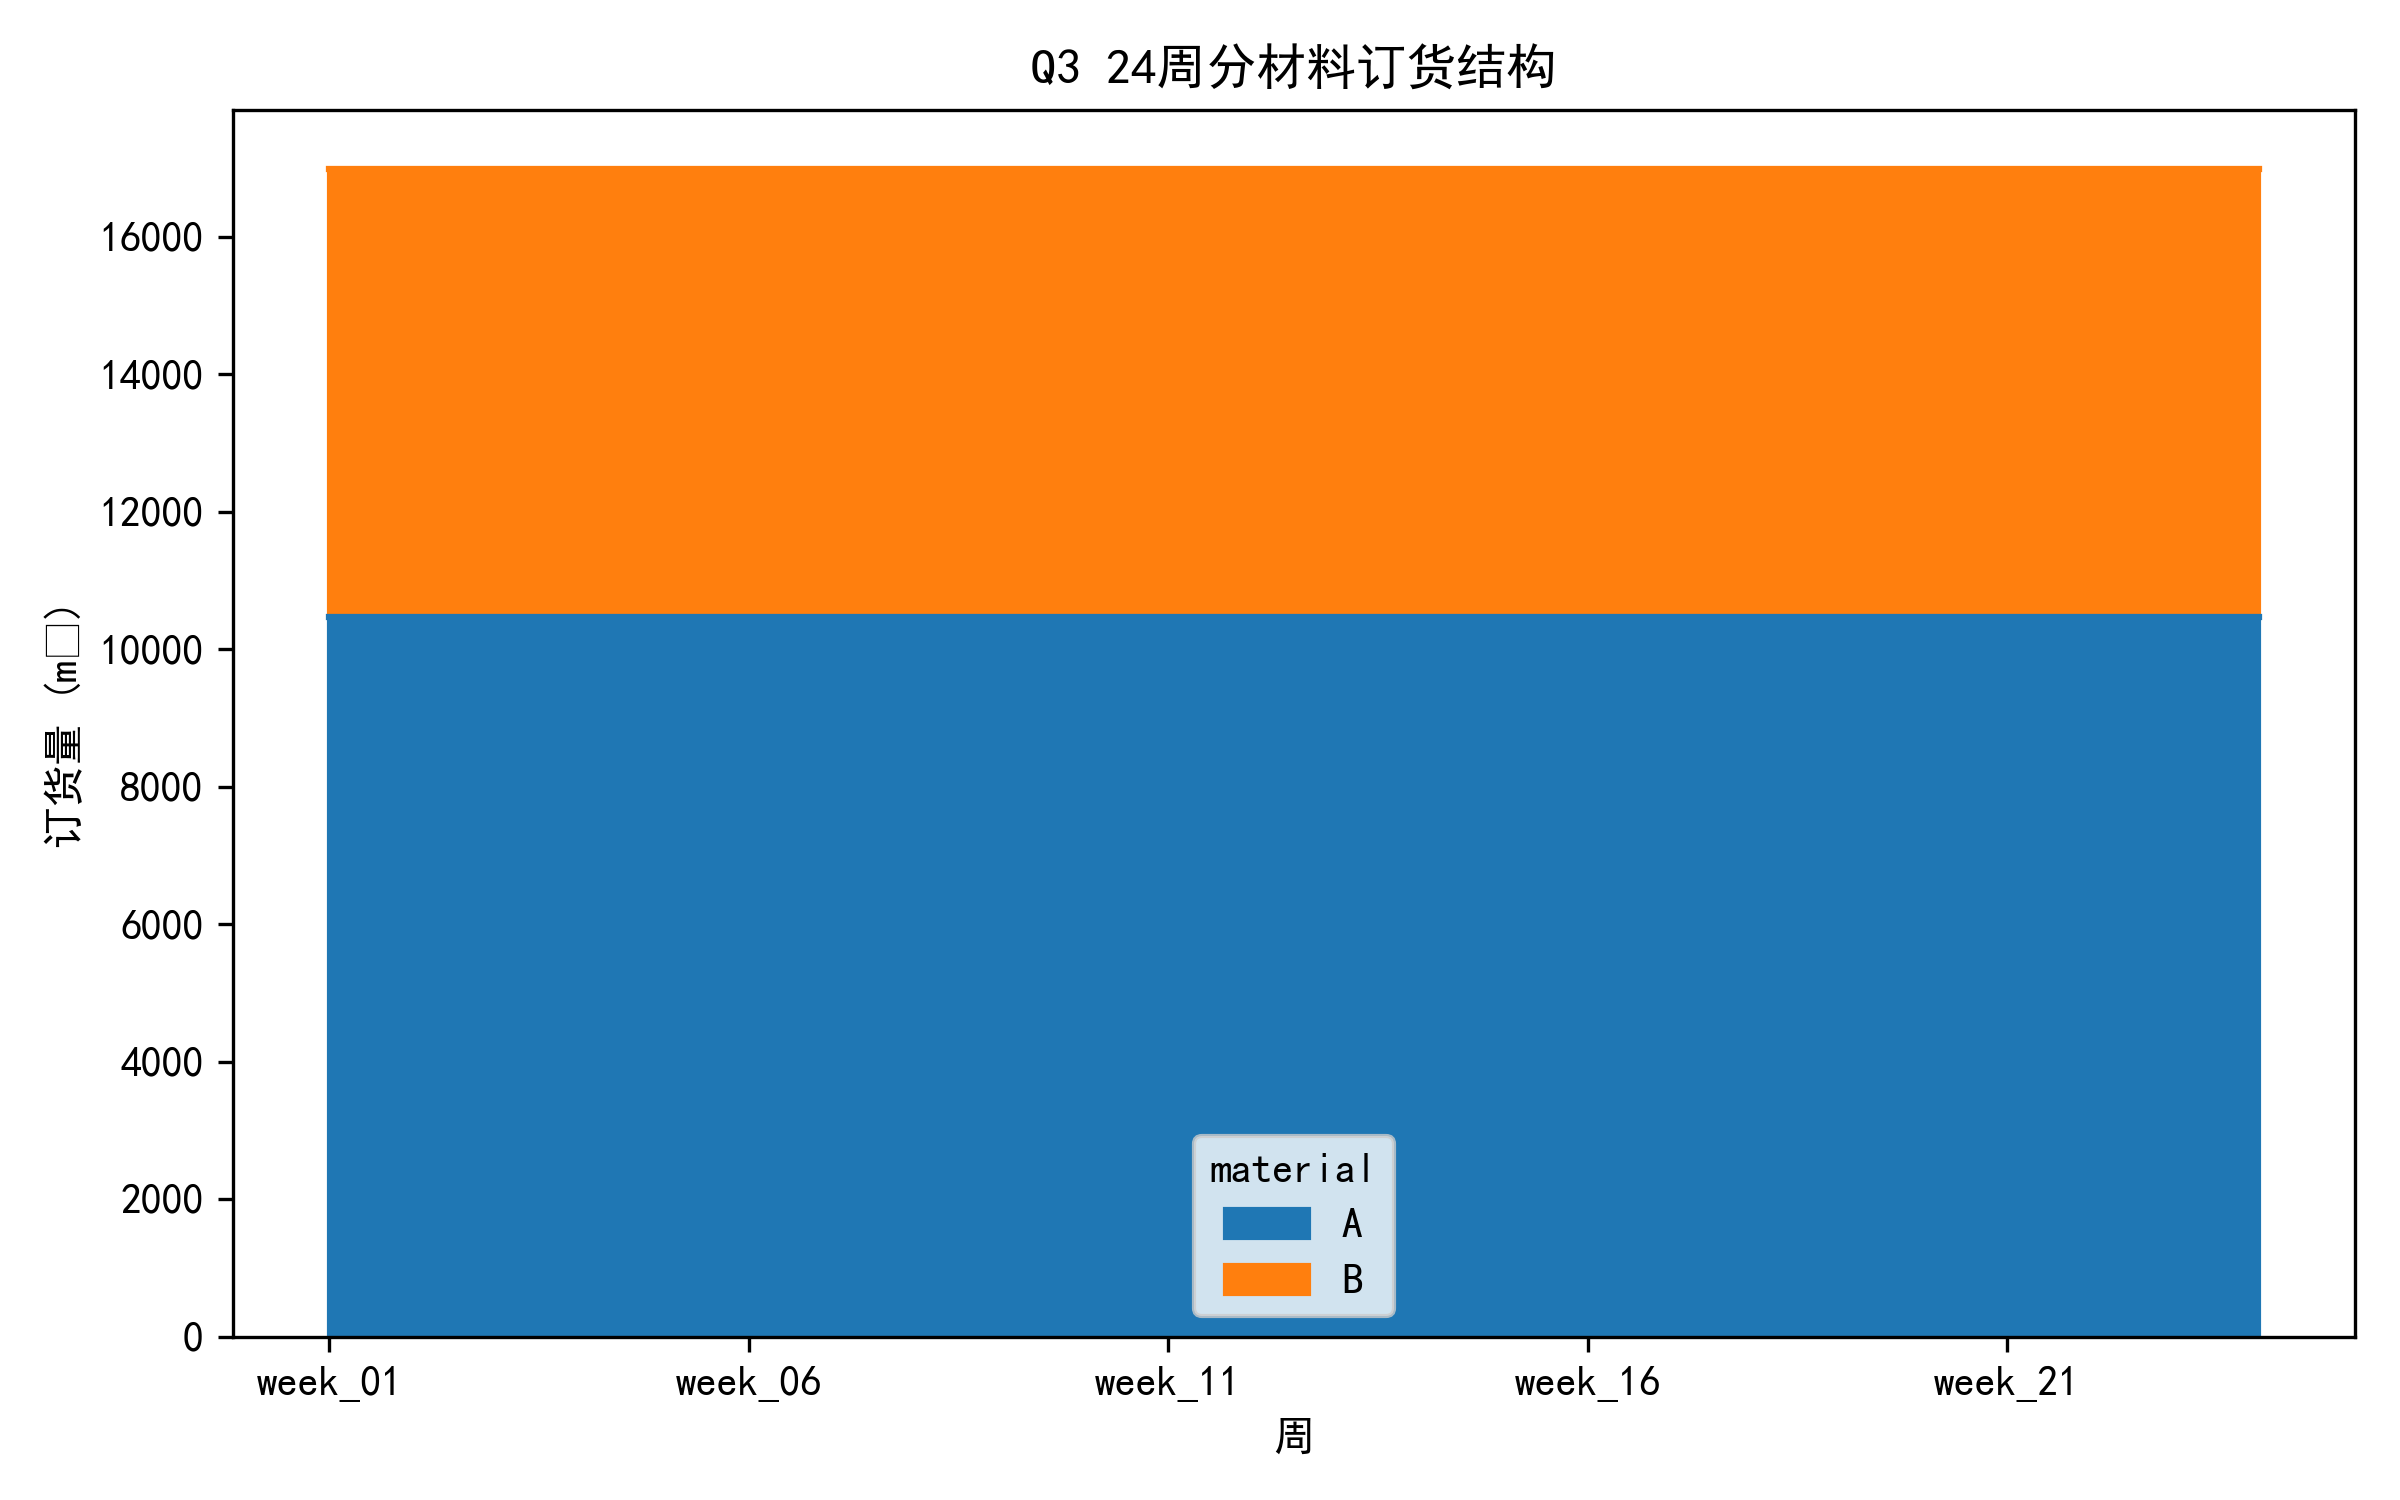
\includegraphics[width=0.78\textwidth]{../output/figures/q3_material_mix.png}
\caption{Q3分材料订货结构（24周）}
\label{fig:q3mix}
\end{figure}

\begin{figure}[H]
\centering
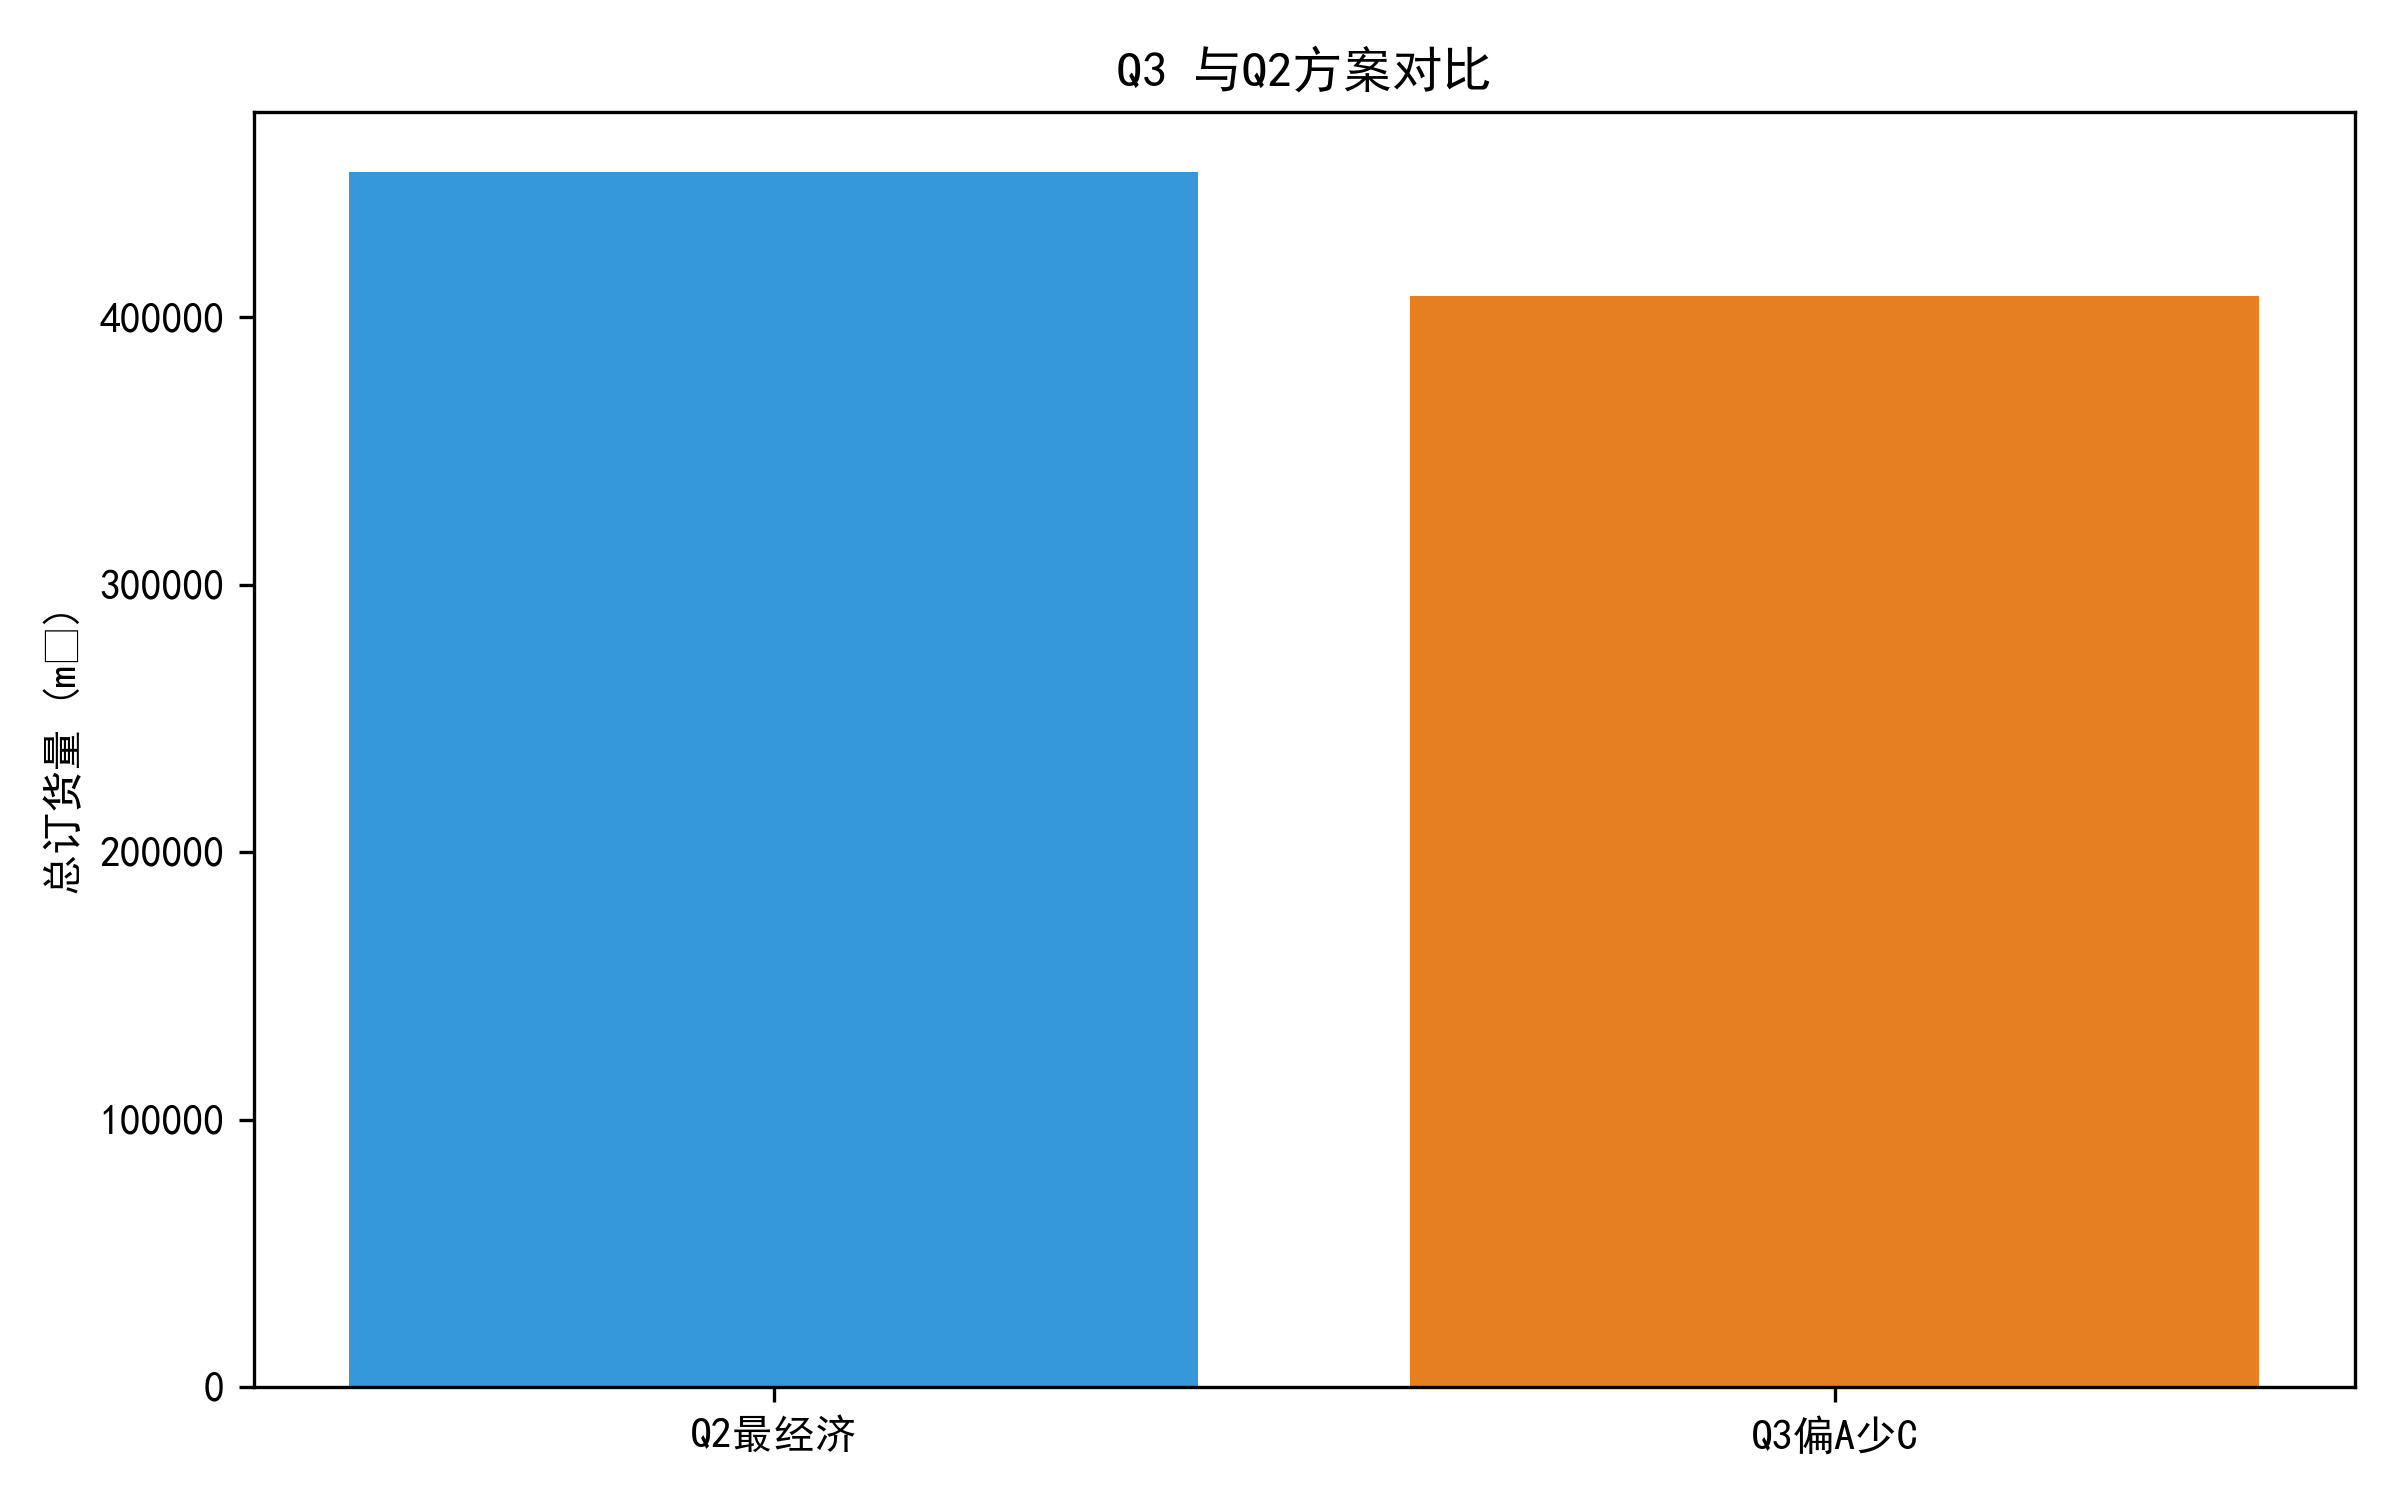
\includegraphics[width=0.72\textwidth]{../output/figures/q3_vs_q2.png}
\caption{Q3与Q2总订货量对比}
\label{fig:q3v2}
\end{figure}


\subsection{问题三小结}
结构优化成功实现“多A少C”：C类产品当量清零，A类显著上升，总订货与成本指数同步下降，符合压缩运仓储成本的题意。转运仍采用损耗优先策略，与问题二形成可对比的一对方案。

\section{问题四：产能可提升幅度与扩产方案}

\subsection{双瓶颈产能模型}
设产能$C(\lambda)=\lambda C_0$。可行需同时满足：
\begin{align}
\sum_{i\in\mathcal{S}}\hat{a}_i &\ge \beta\, C(\lambda)\, e_{\mathrm{eff}},\\
8U &\ge C(\lambda)\, e_{\mathrm{eff}},
\end{align}
其中$e_{\mathrm{eff}}$为所选材料结构下的有效消耗。转运总运力上界为$8\times6000=48000\,\mathrm{m}^3$/周，构成硬约束。对$\lambda$作二分搜索，每次调用与问题二同类的可行性/订购程序，得到最大可行$\lambda^*$。

\subsection{结果与瓶颈分解}
计算得$\lambda^*=2.4996$，提升后周产能70489\,m$^3$（+150.0\%），方案动用402家供应商。瓶颈分解见表\ref{tab:bn}与图\ref{fig:bn}：在高倍增情形下，供应端需几乎动用全部供应商，转运端接近满负荷，二者共同限制继续扩张。

\begin{table}[H]
\centering
\caption{Q4产能瓶颈分解（周原材料量）}
\label{tab:bn}
\begin{tabular}{lr}
\toprule
瓶颈项 & 周原材料量(m$^3$) \\
\midrule
供应商供货能力(周) & 35958.4 \\
转运能力8×6000 & 48000.0 \\
Q4方案周需求(A当量近似) & 42293.2 \\
\bottomrule
\end{tabular}
\end{table}

\begin{figure}[H]
\centering
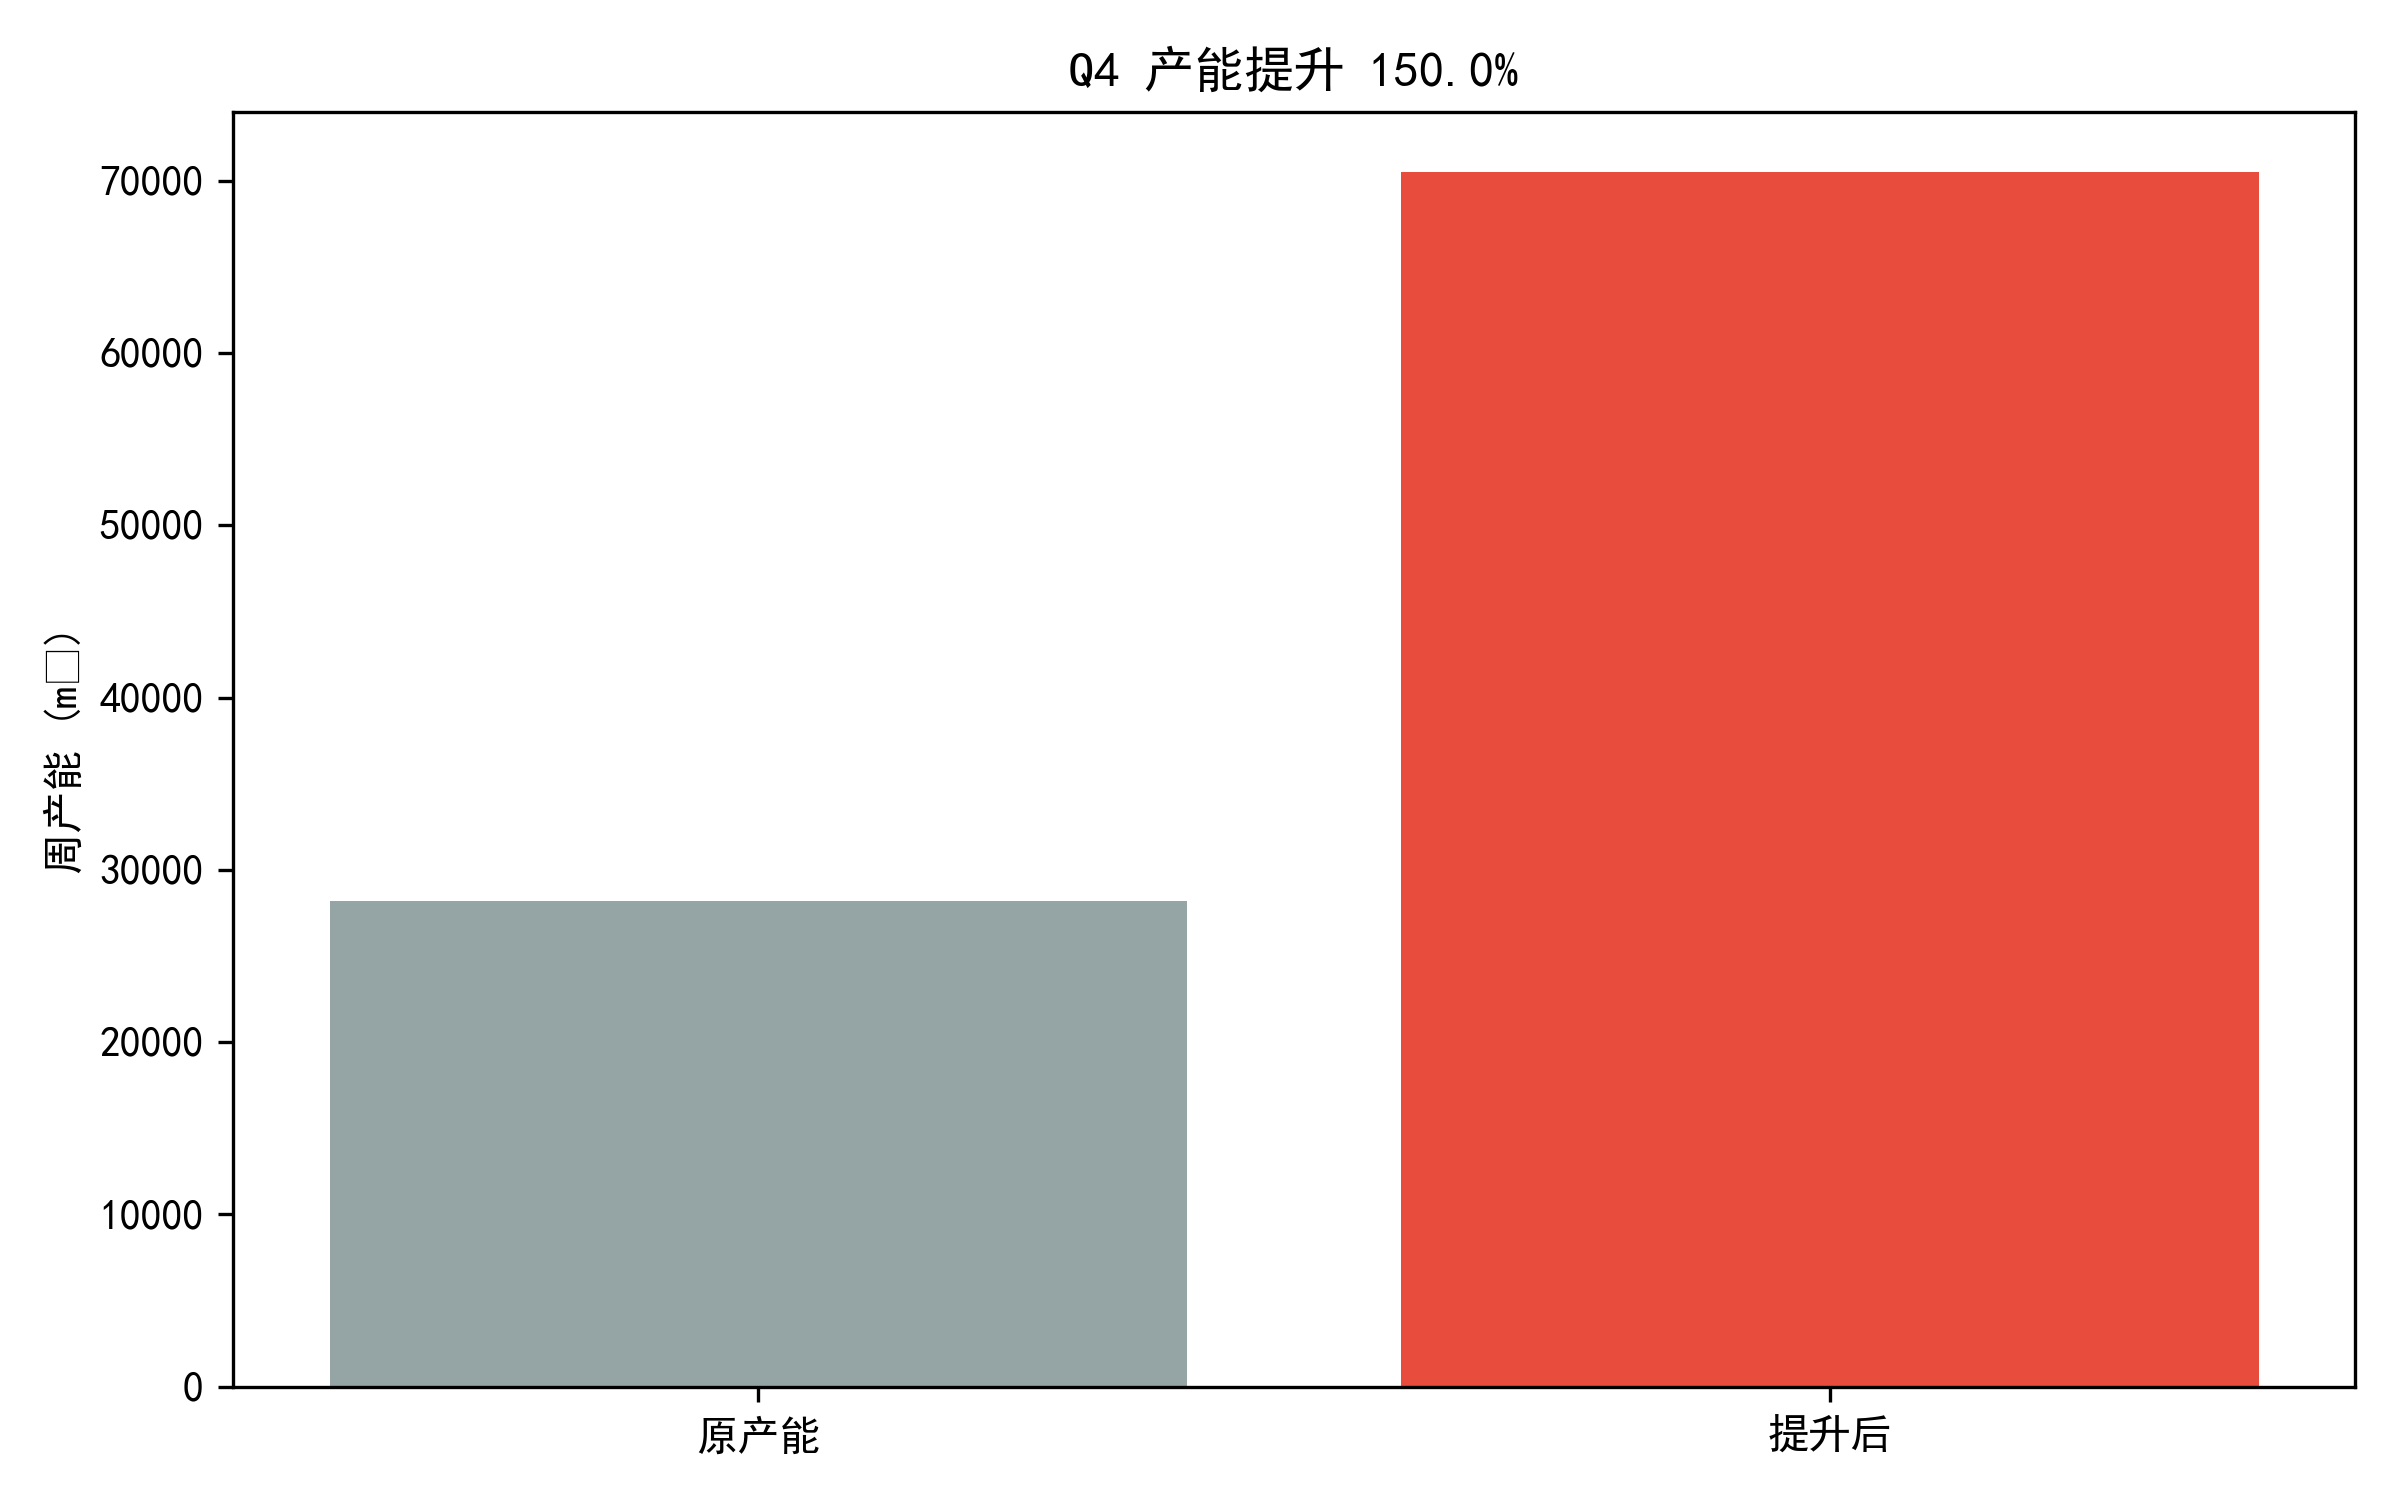
\includegraphics[width=0.72\textwidth]{../output/figures/q4_capacity_compare.png}
\caption{产能提升前后对比}
\label{fig:q4cap}
\end{figure}

\begin{figure}[H]
\centering
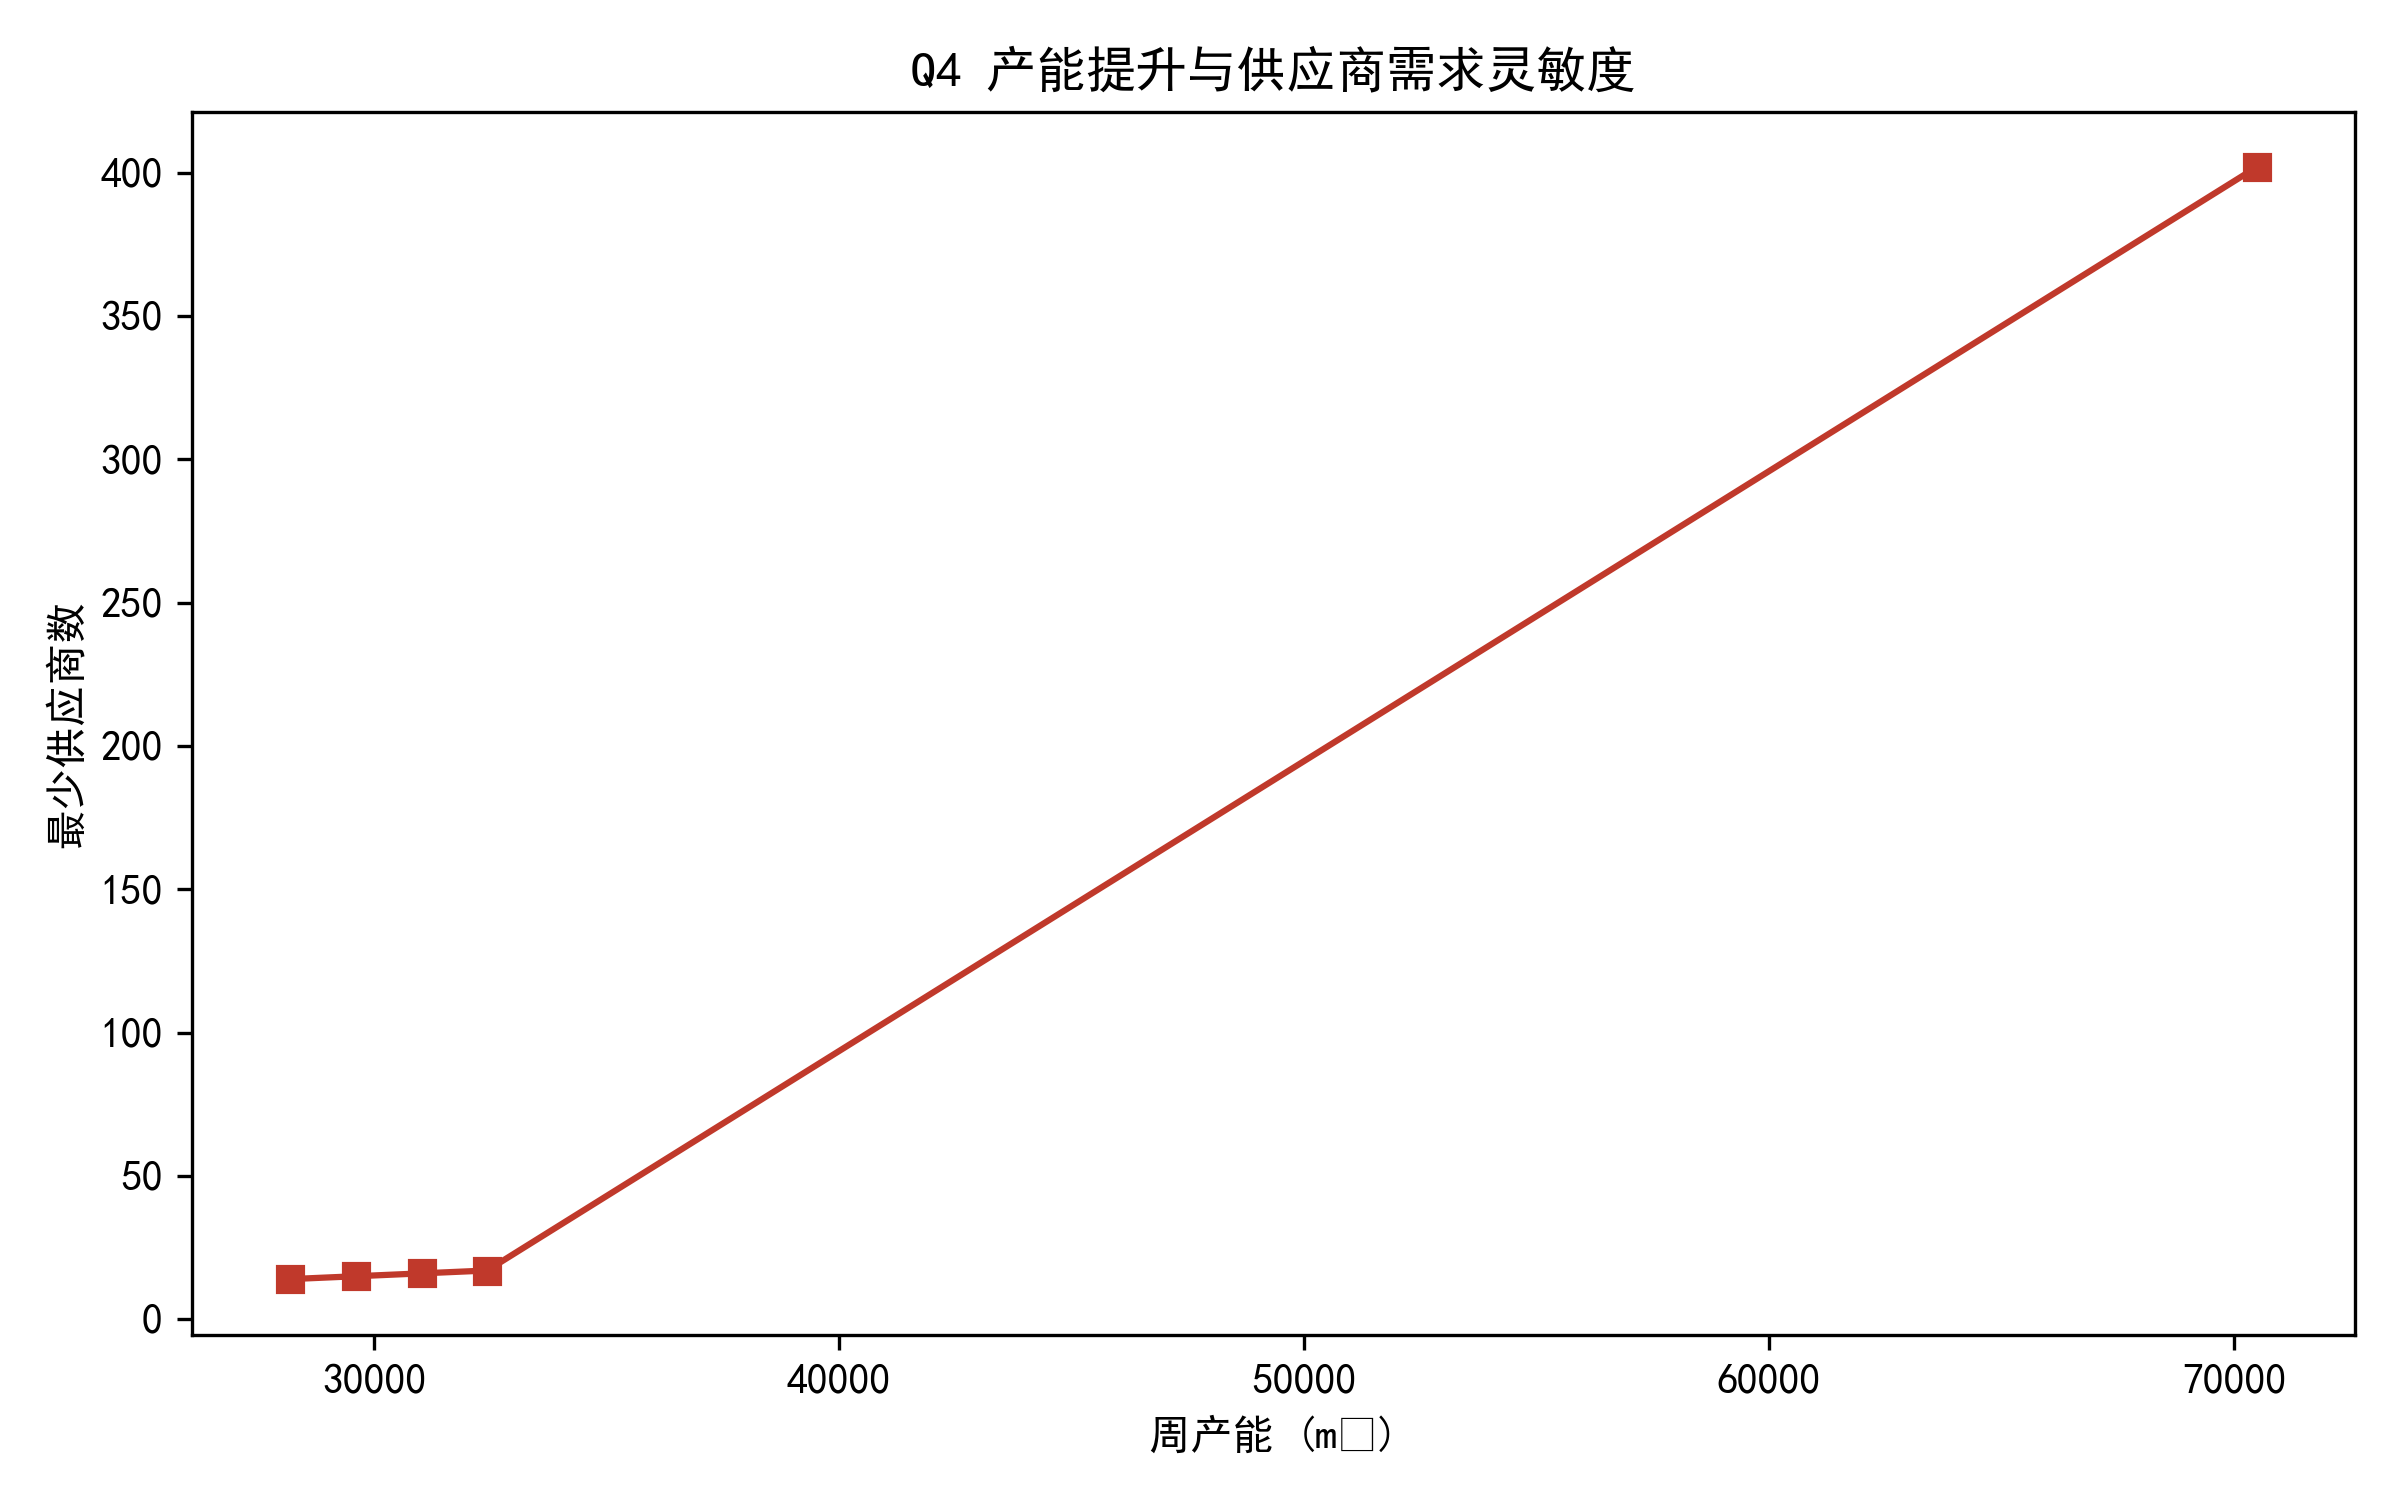
\includegraphics[width=0.78\textwidth]{../output/figures/q4_capacity_sensitivity.png}
\caption{产能—最少供应商数灵敏度}
\label{fig:q4sens}
\end{figure}

\begin{figure}[H]
\centering
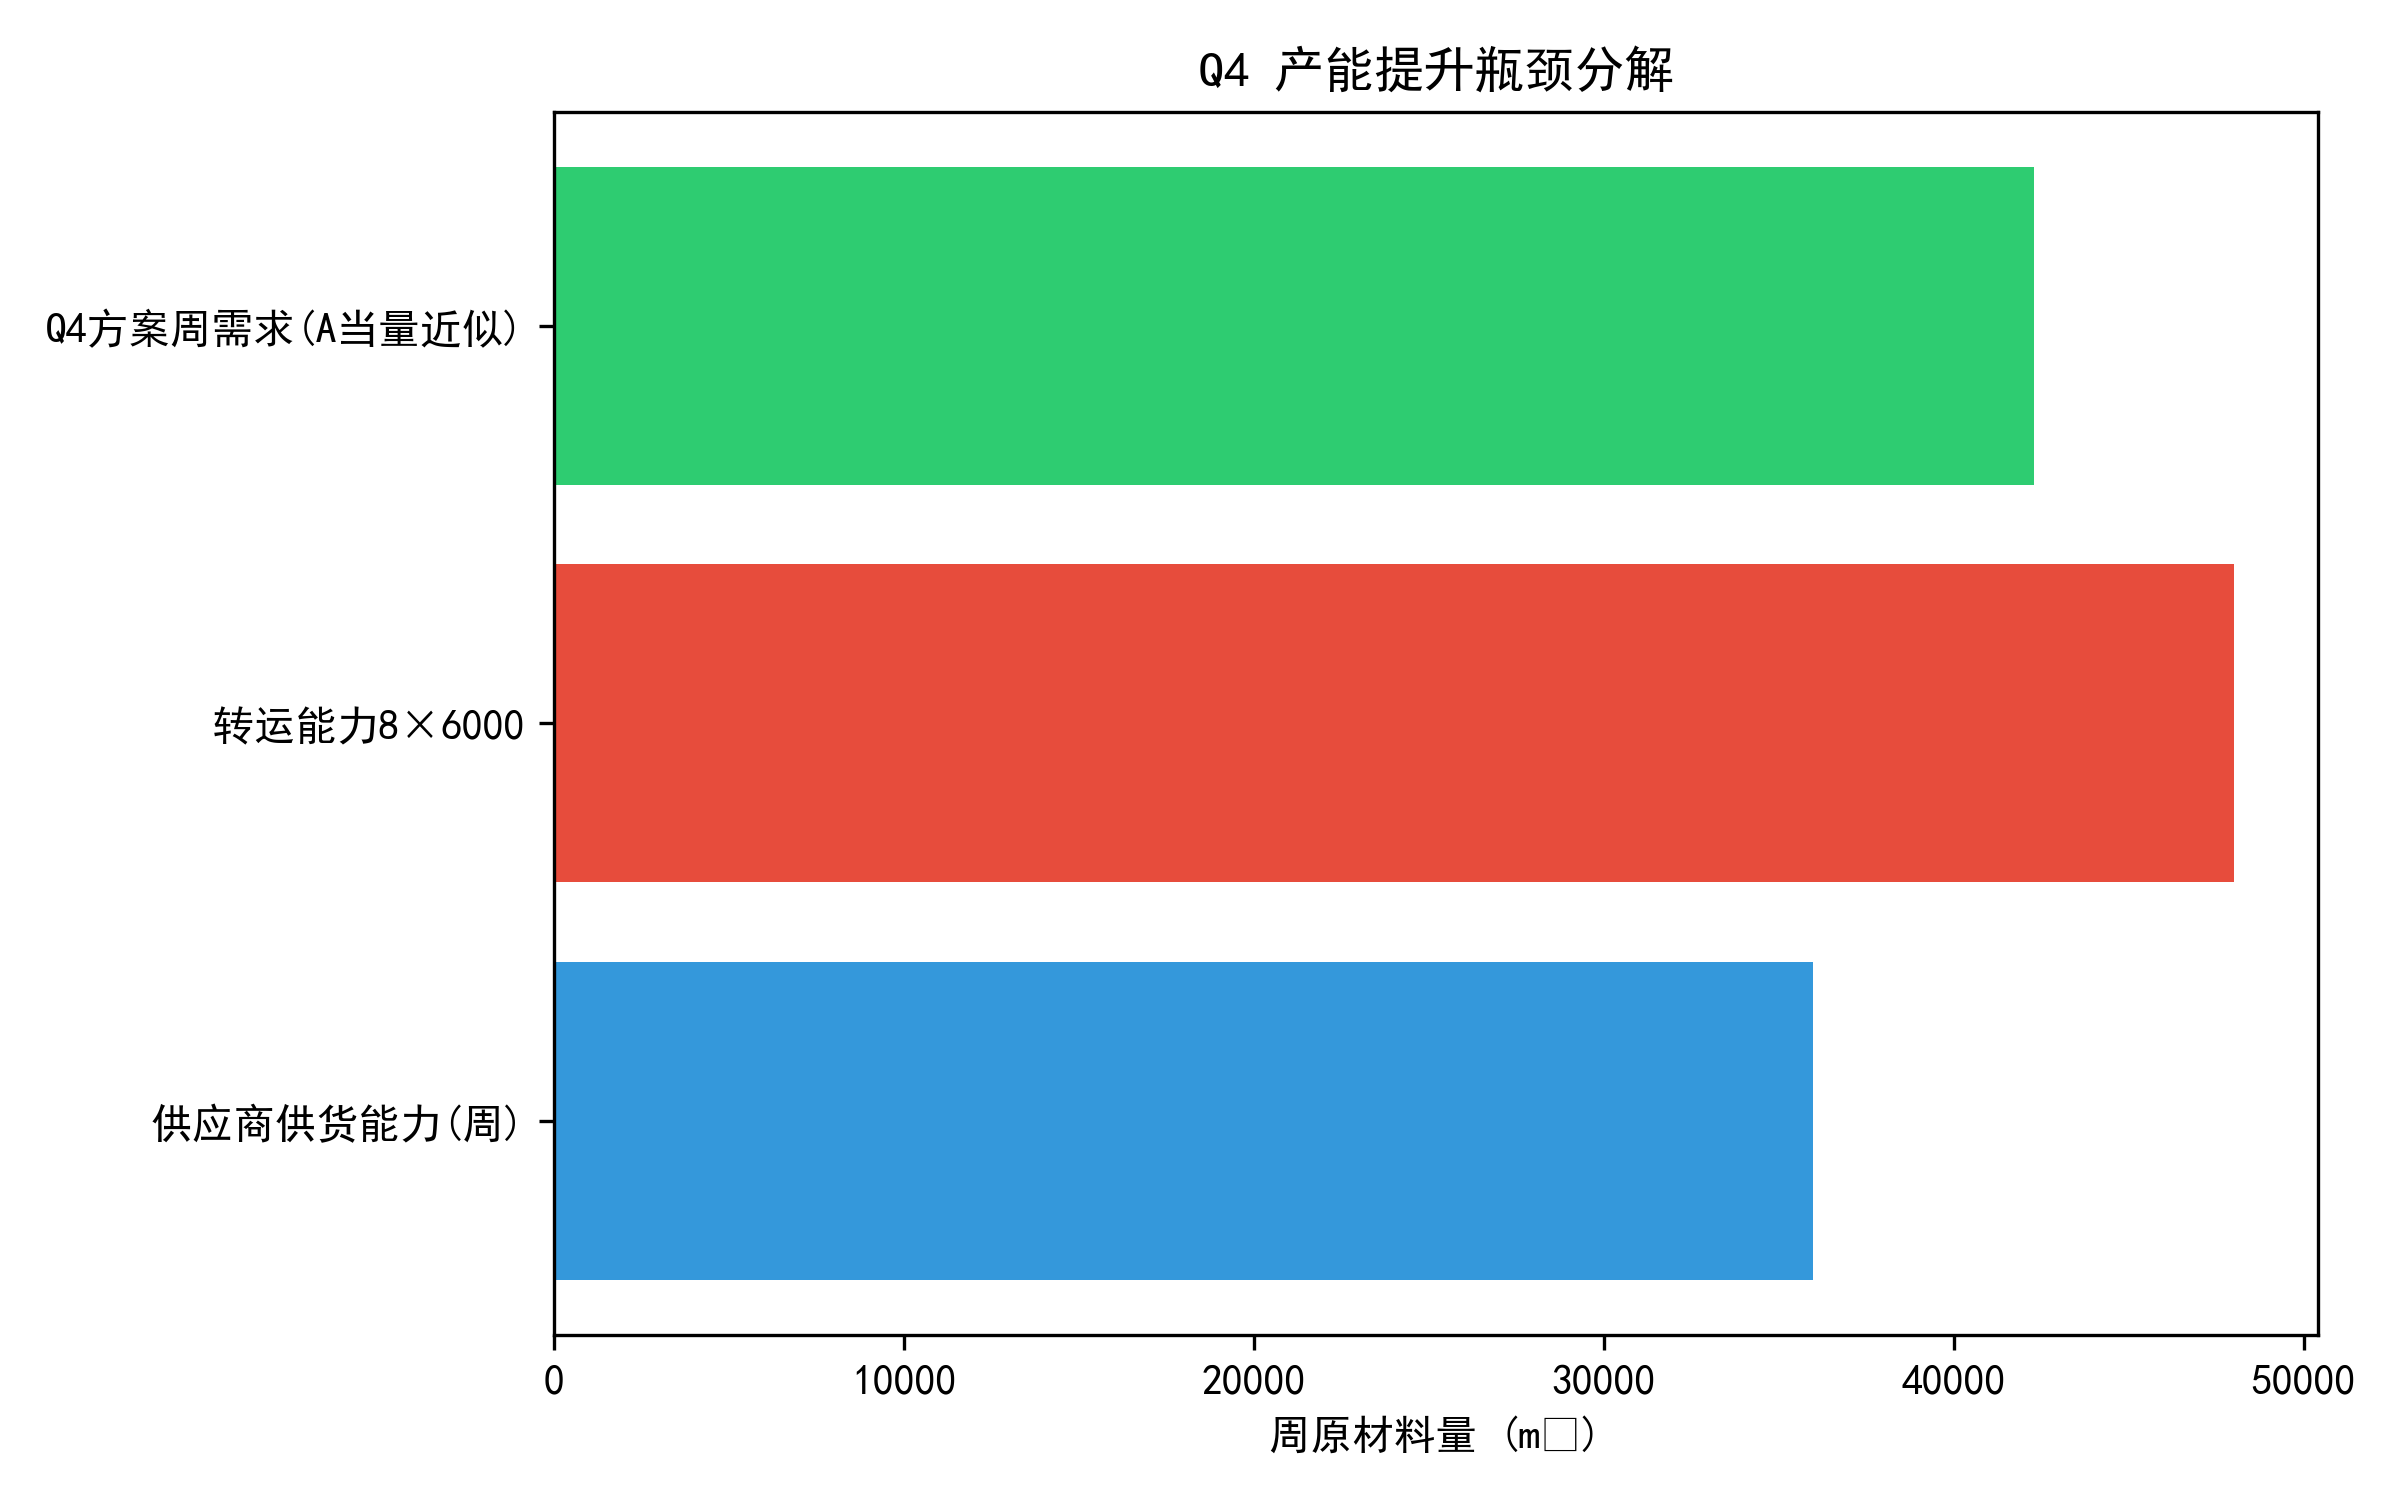
\includegraphics[width=0.78\textwidth]{../output/figures/q4_bottleneck.png}
\caption{Q4产能提升瓶颈分解}
\label{fig:bn}
\end{figure}


\subsection{问题四小结}
在现有供应商与转运商条件下，周产能理论可提升约150.0\%；但需扩大供应商集合并接近转运上限，实际落地应预留冗余并关注损耗波动。

\section{模型检验：对比、灵敏度与鲁棒性}

\subsection{有效性：多方法与基准对比}
\begin{itemize}[leftmargin=2em]
\item Q1：熵权-TOPSIS相对累计供货基准，Top50平均满足率由1.024变为1.041，更强调履约质量；
\item 多方法Top50重叠普遍较高，说明核心集合稳定；
\item Q2/Q3消融对比（表\ref{tab:q23}）显示结构偏好带来可量化的体积与成本变化。
\end{itemize}

\subsection{灵敏度分析}
（1）\textbf{Q1权重扰动}：对满足率权重施加$\pm30\%$扰动并重归一，观察Top50重叠（图\ref{fig:q1sens}）。\\
（2）\textbf{Q2价格灵敏度}：A类相对价格变动时成本指数近似线性响应（图\ref{fig:q2price}）。\\
（3）\textbf{Q4产能灵敏度}：随$\lambda$增大，所需最少供应商数上升（图\ref{fig:q4sens}）。

\begin{figure}[H]
\centering
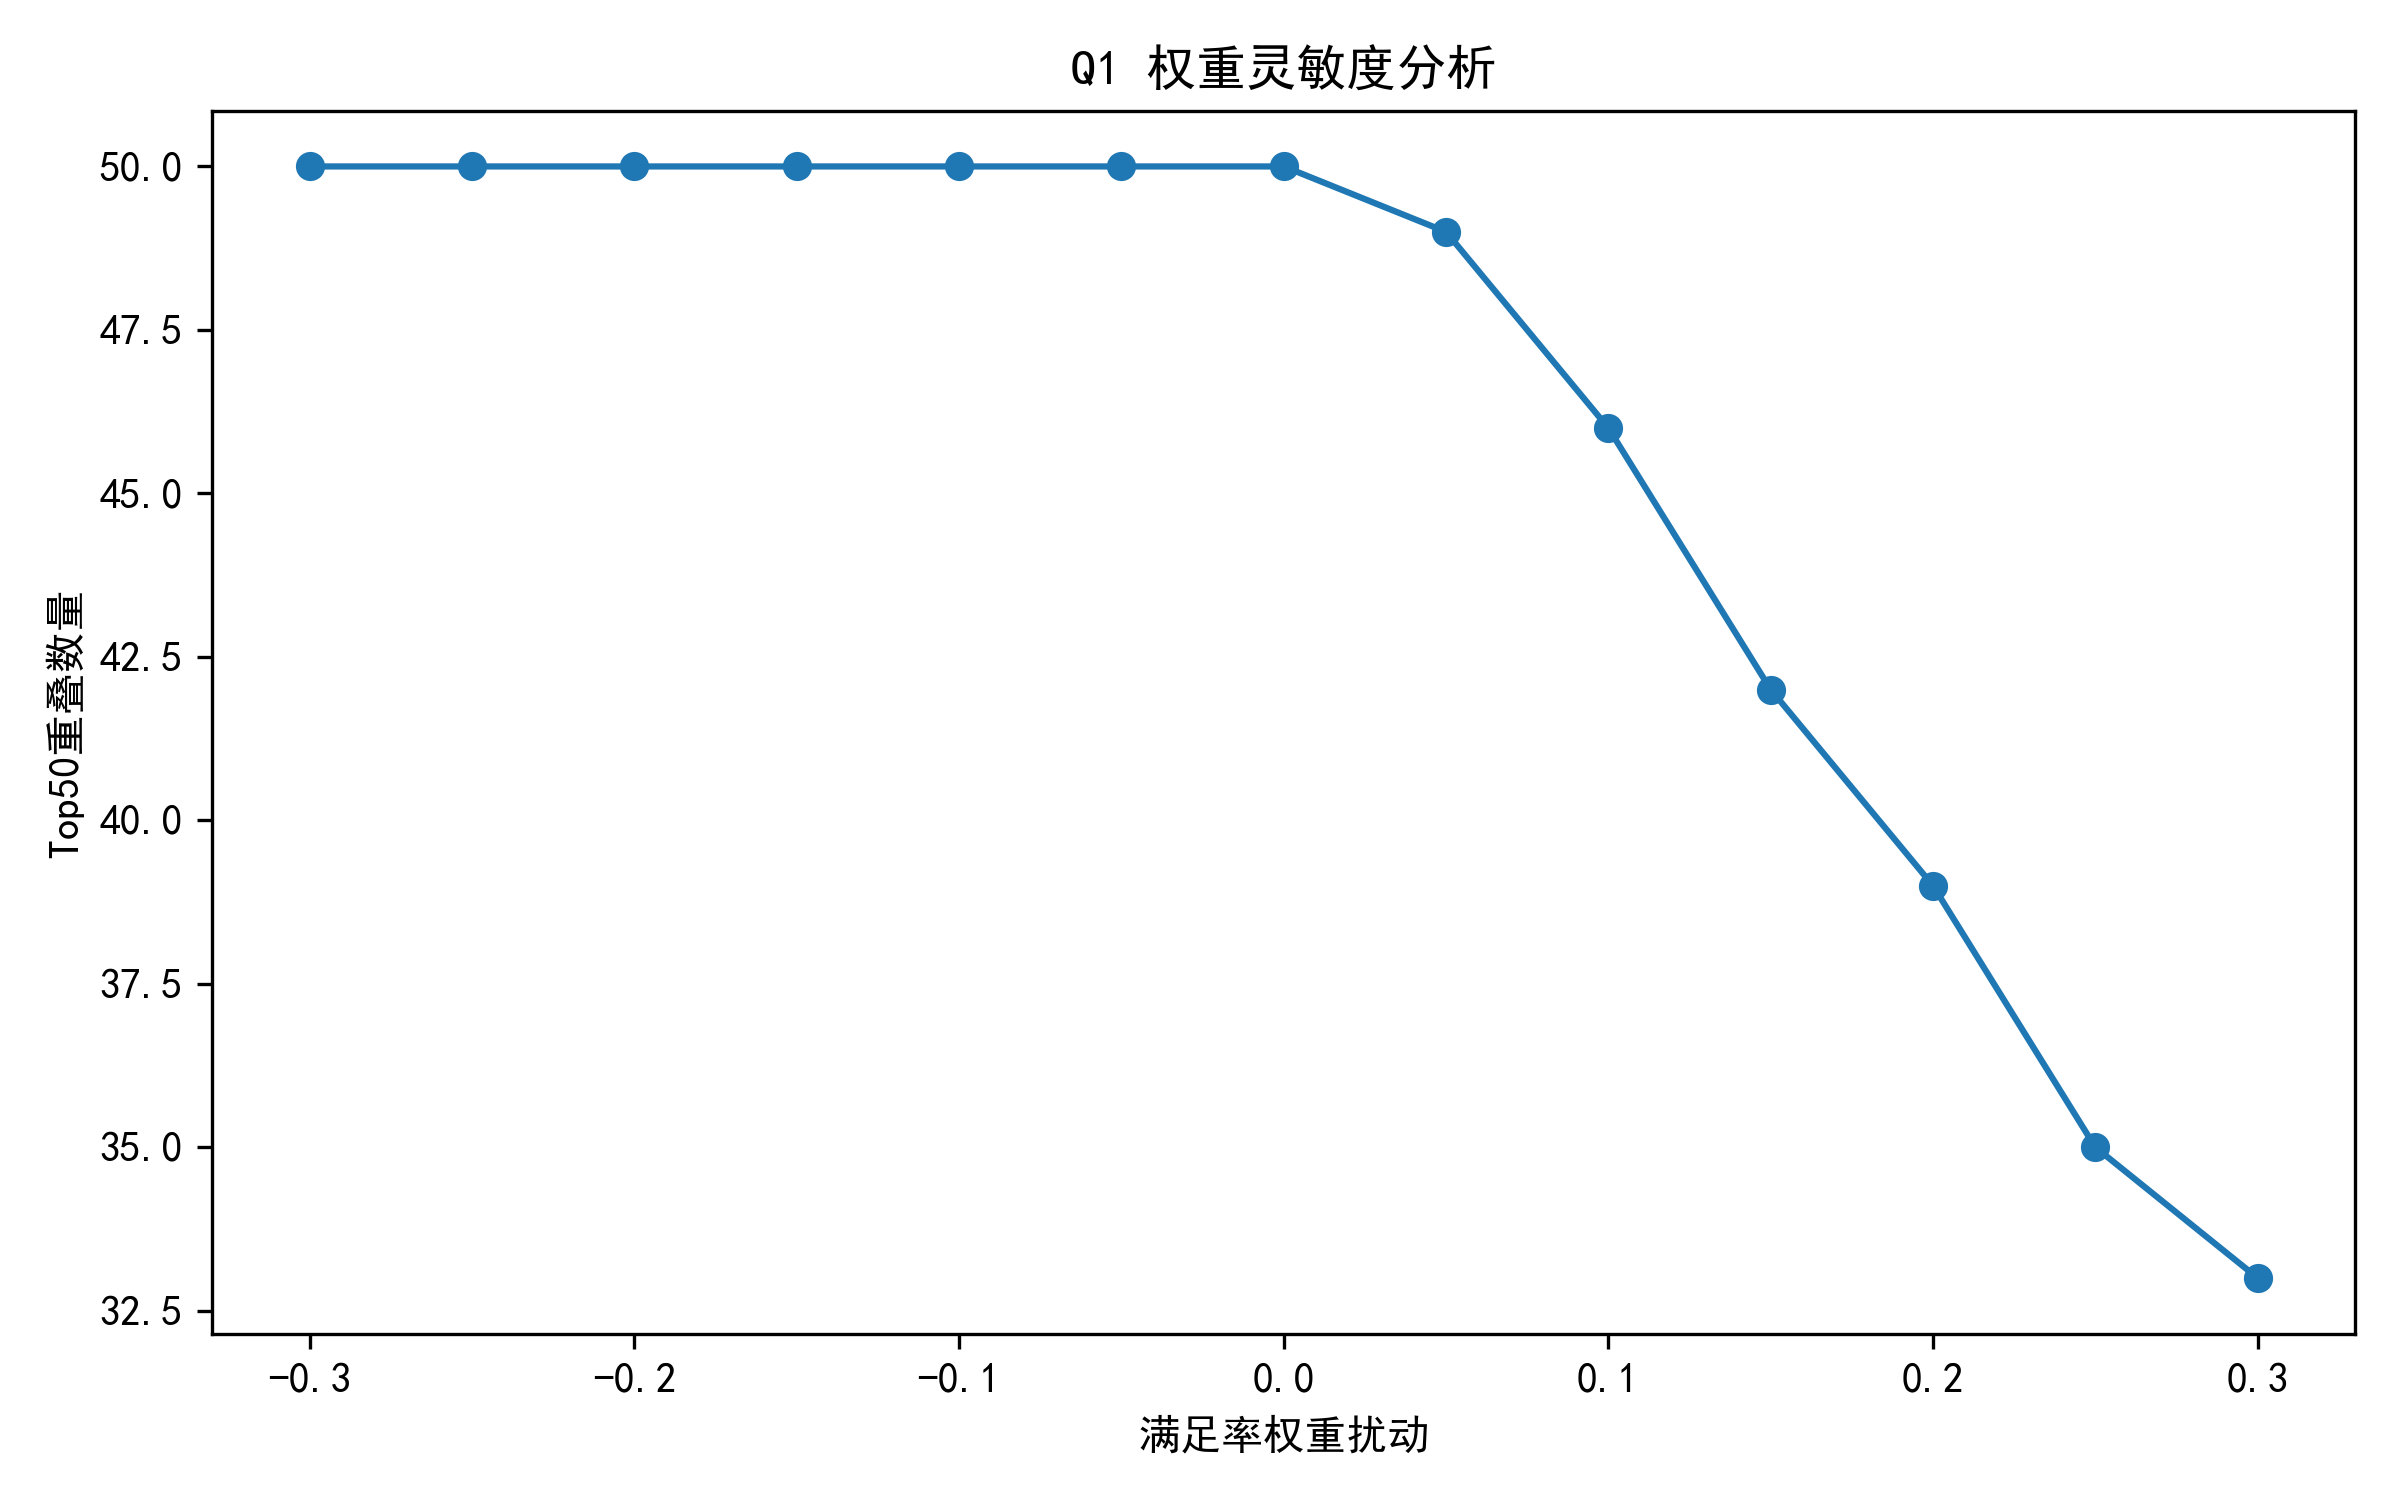
\includegraphics[width=0.75\textwidth]{../output/figures/q1_sensitivity.png}
\caption{Q1满足率权重扰动下的Top50重叠}
\label{fig:q1sens}
\end{figure}


\subsection{鲁棒性检验}
\textbf{评价鲁棒性：}对满足率、稳定性、周均供货施加正态乘性噪声，蒙特卡洛$n=200$次重排序。Top50平均重叠49.34，5\%分位49，平均Jaccard=0.974（图\ref{fig:mc}），表明评价对中等噪声不敏感。

\textbf{库存鲁棒性：}在订购方案固定下，对履约率加噪声模拟库存路径，统计库存跌破两周线的周数与概率（表\ref{tab:rob}，图\ref{fig:rob}）。结果显示在10\%噪声水平下方案仍具较好抗扰性；噪声增大到15\%时风险上升，提示实务中应保留额外安全裕度或滚动重优化。

\begin{table}[H]
\centering
\caption{订购方案库存鲁棒性（蒙特卡洛）}
\label{tab:rob}
\begin{tabular}{lcccc}
\toprule
方案 & 扰动强度 & 平均不足周数 & 不足概率 & 平均最低库存 \\
\midrule
Q2 & 0.05 & 0.00 & 0.000 & 56400 \\
Q2 & 0.10 & 0.14 & 0.075 & 56347 \\
Q2 & 0.15 & 0.44 & 0.200 & 56181 \\
Q3 & 0.05 & 24.00 & 1.000 & 35872 \\
Q3 & 0.10 & 23.76 & 1.000 & 35923 \\
Q3 & 0.15 & 23.24 & 1.000 & 35795 \\
\bottomrule
\end{tabular}
\end{table}

\begin{figure}[H]
\centering
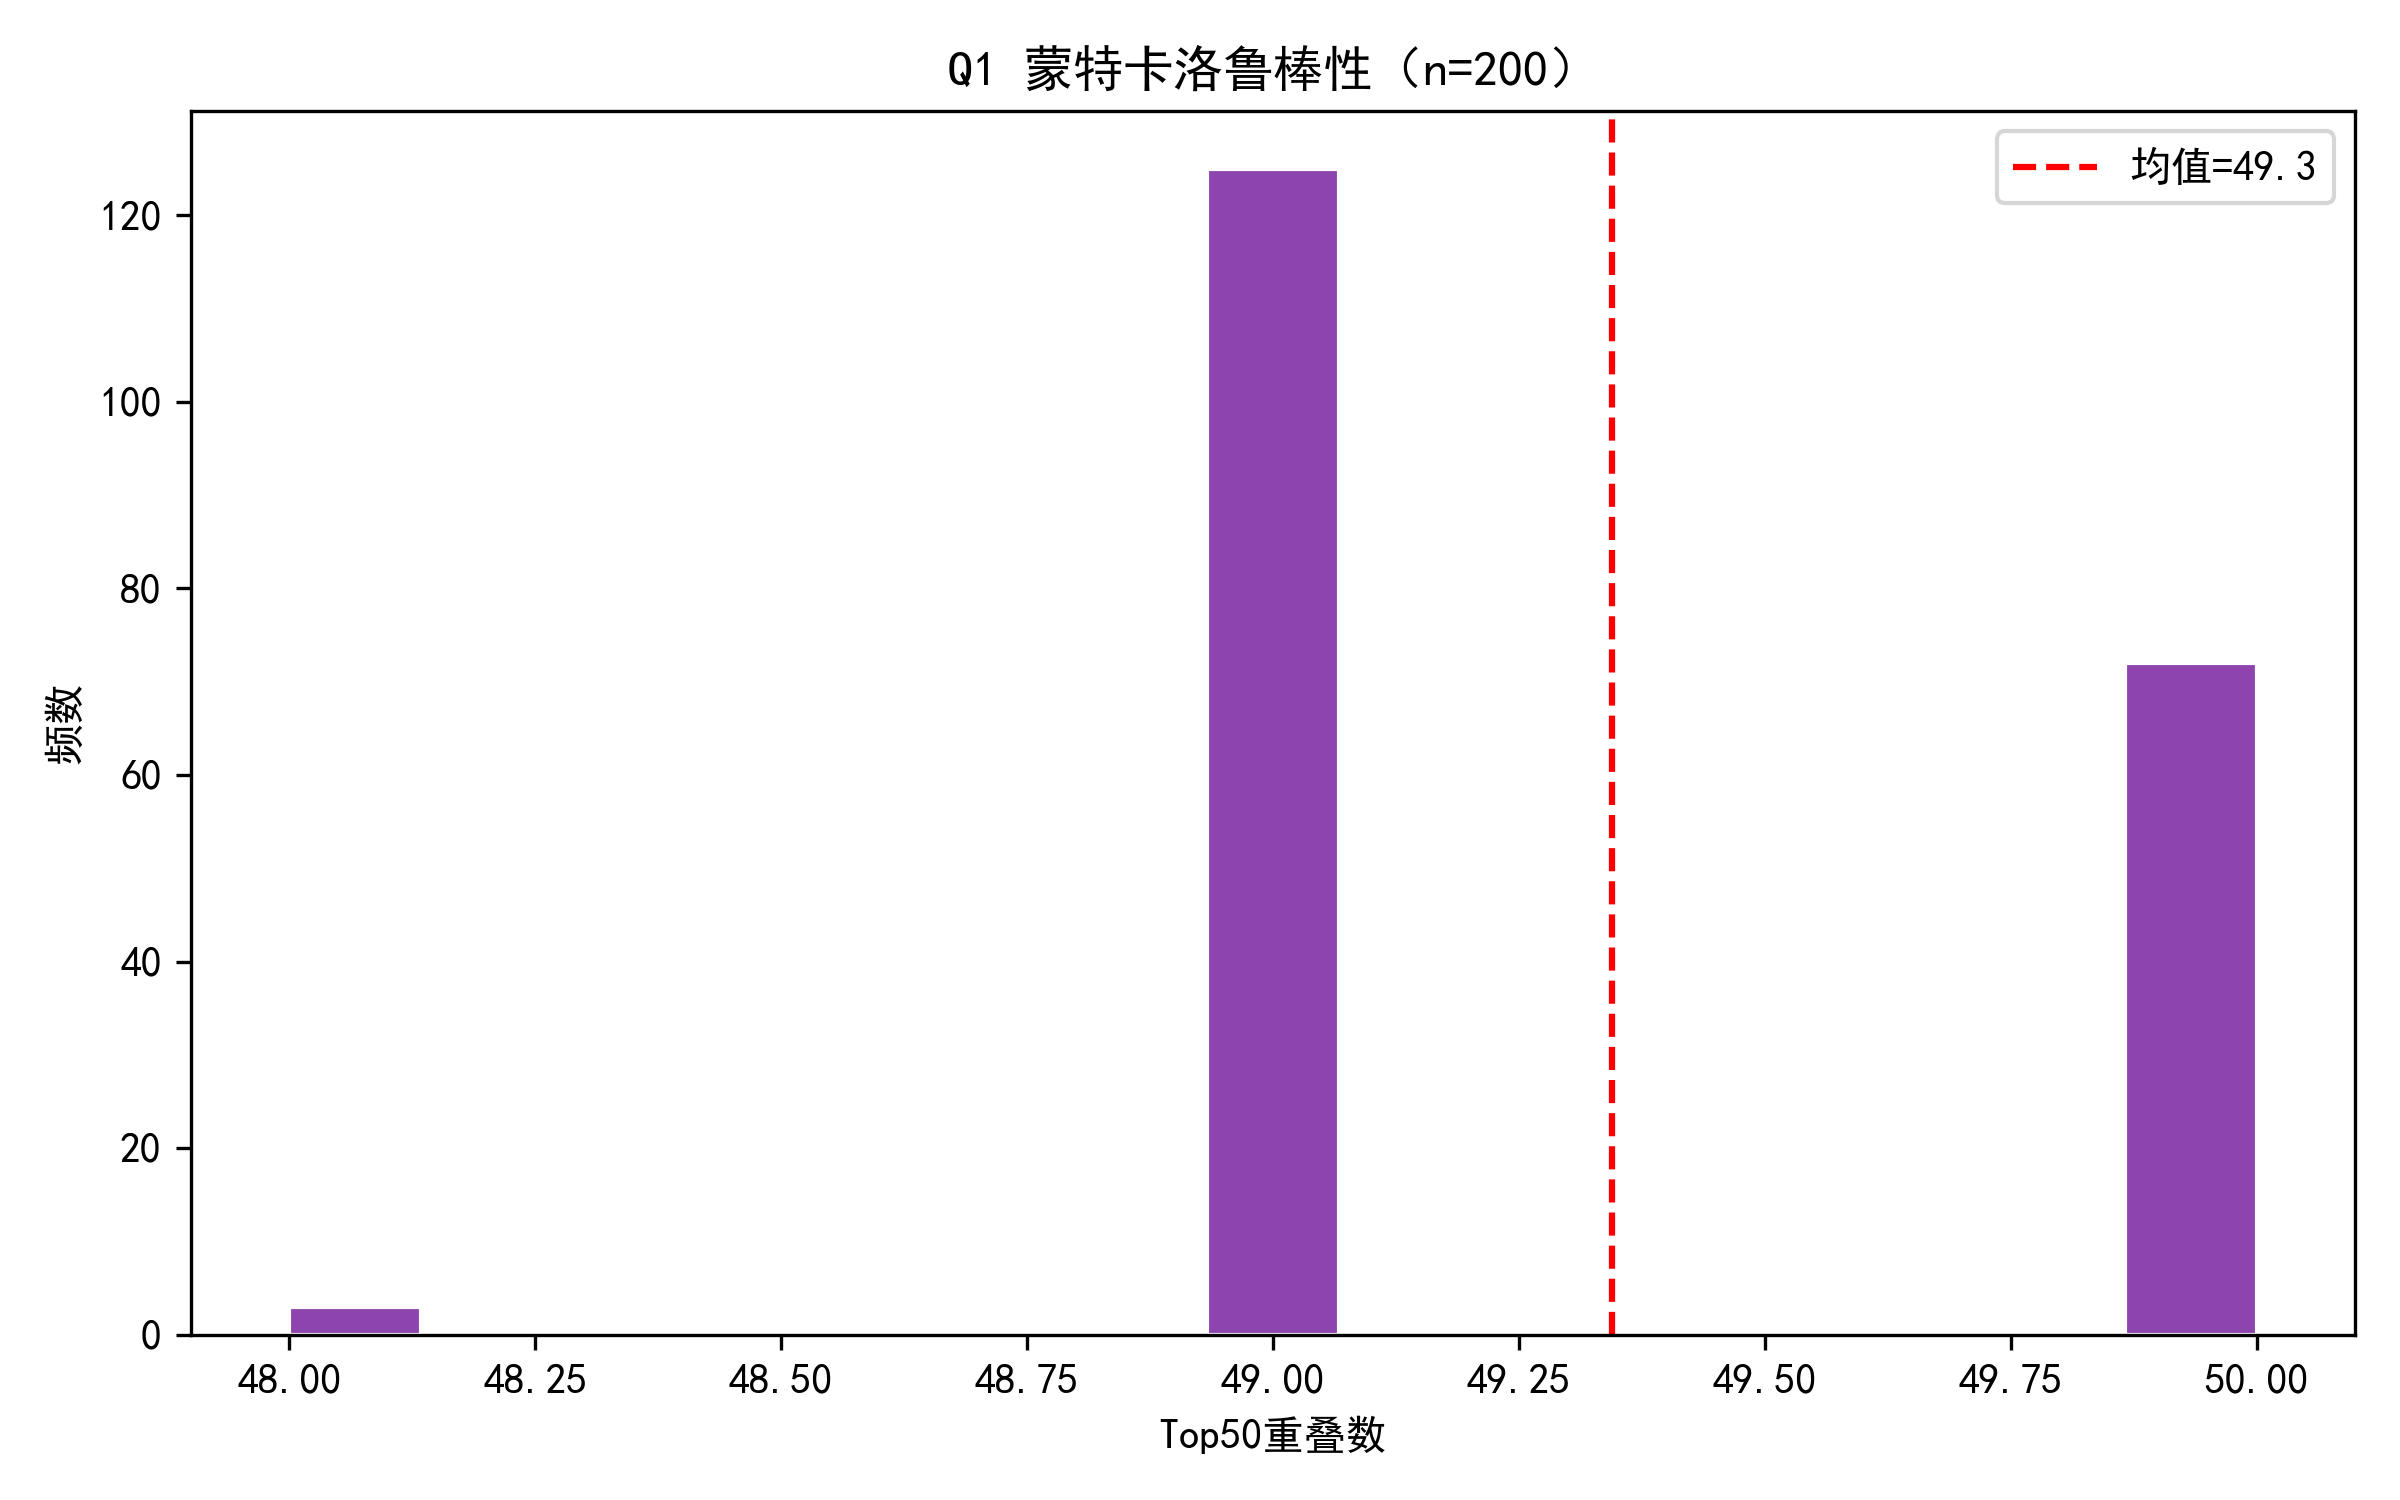
\includegraphics[width=0.75\textwidth]{../output/figures/q1_monte_carlo.png}
\caption{Q1蒙特卡洛Top50重叠分布}
\label{fig:mc}
\end{figure}

\begin{figure}[H]
\centering
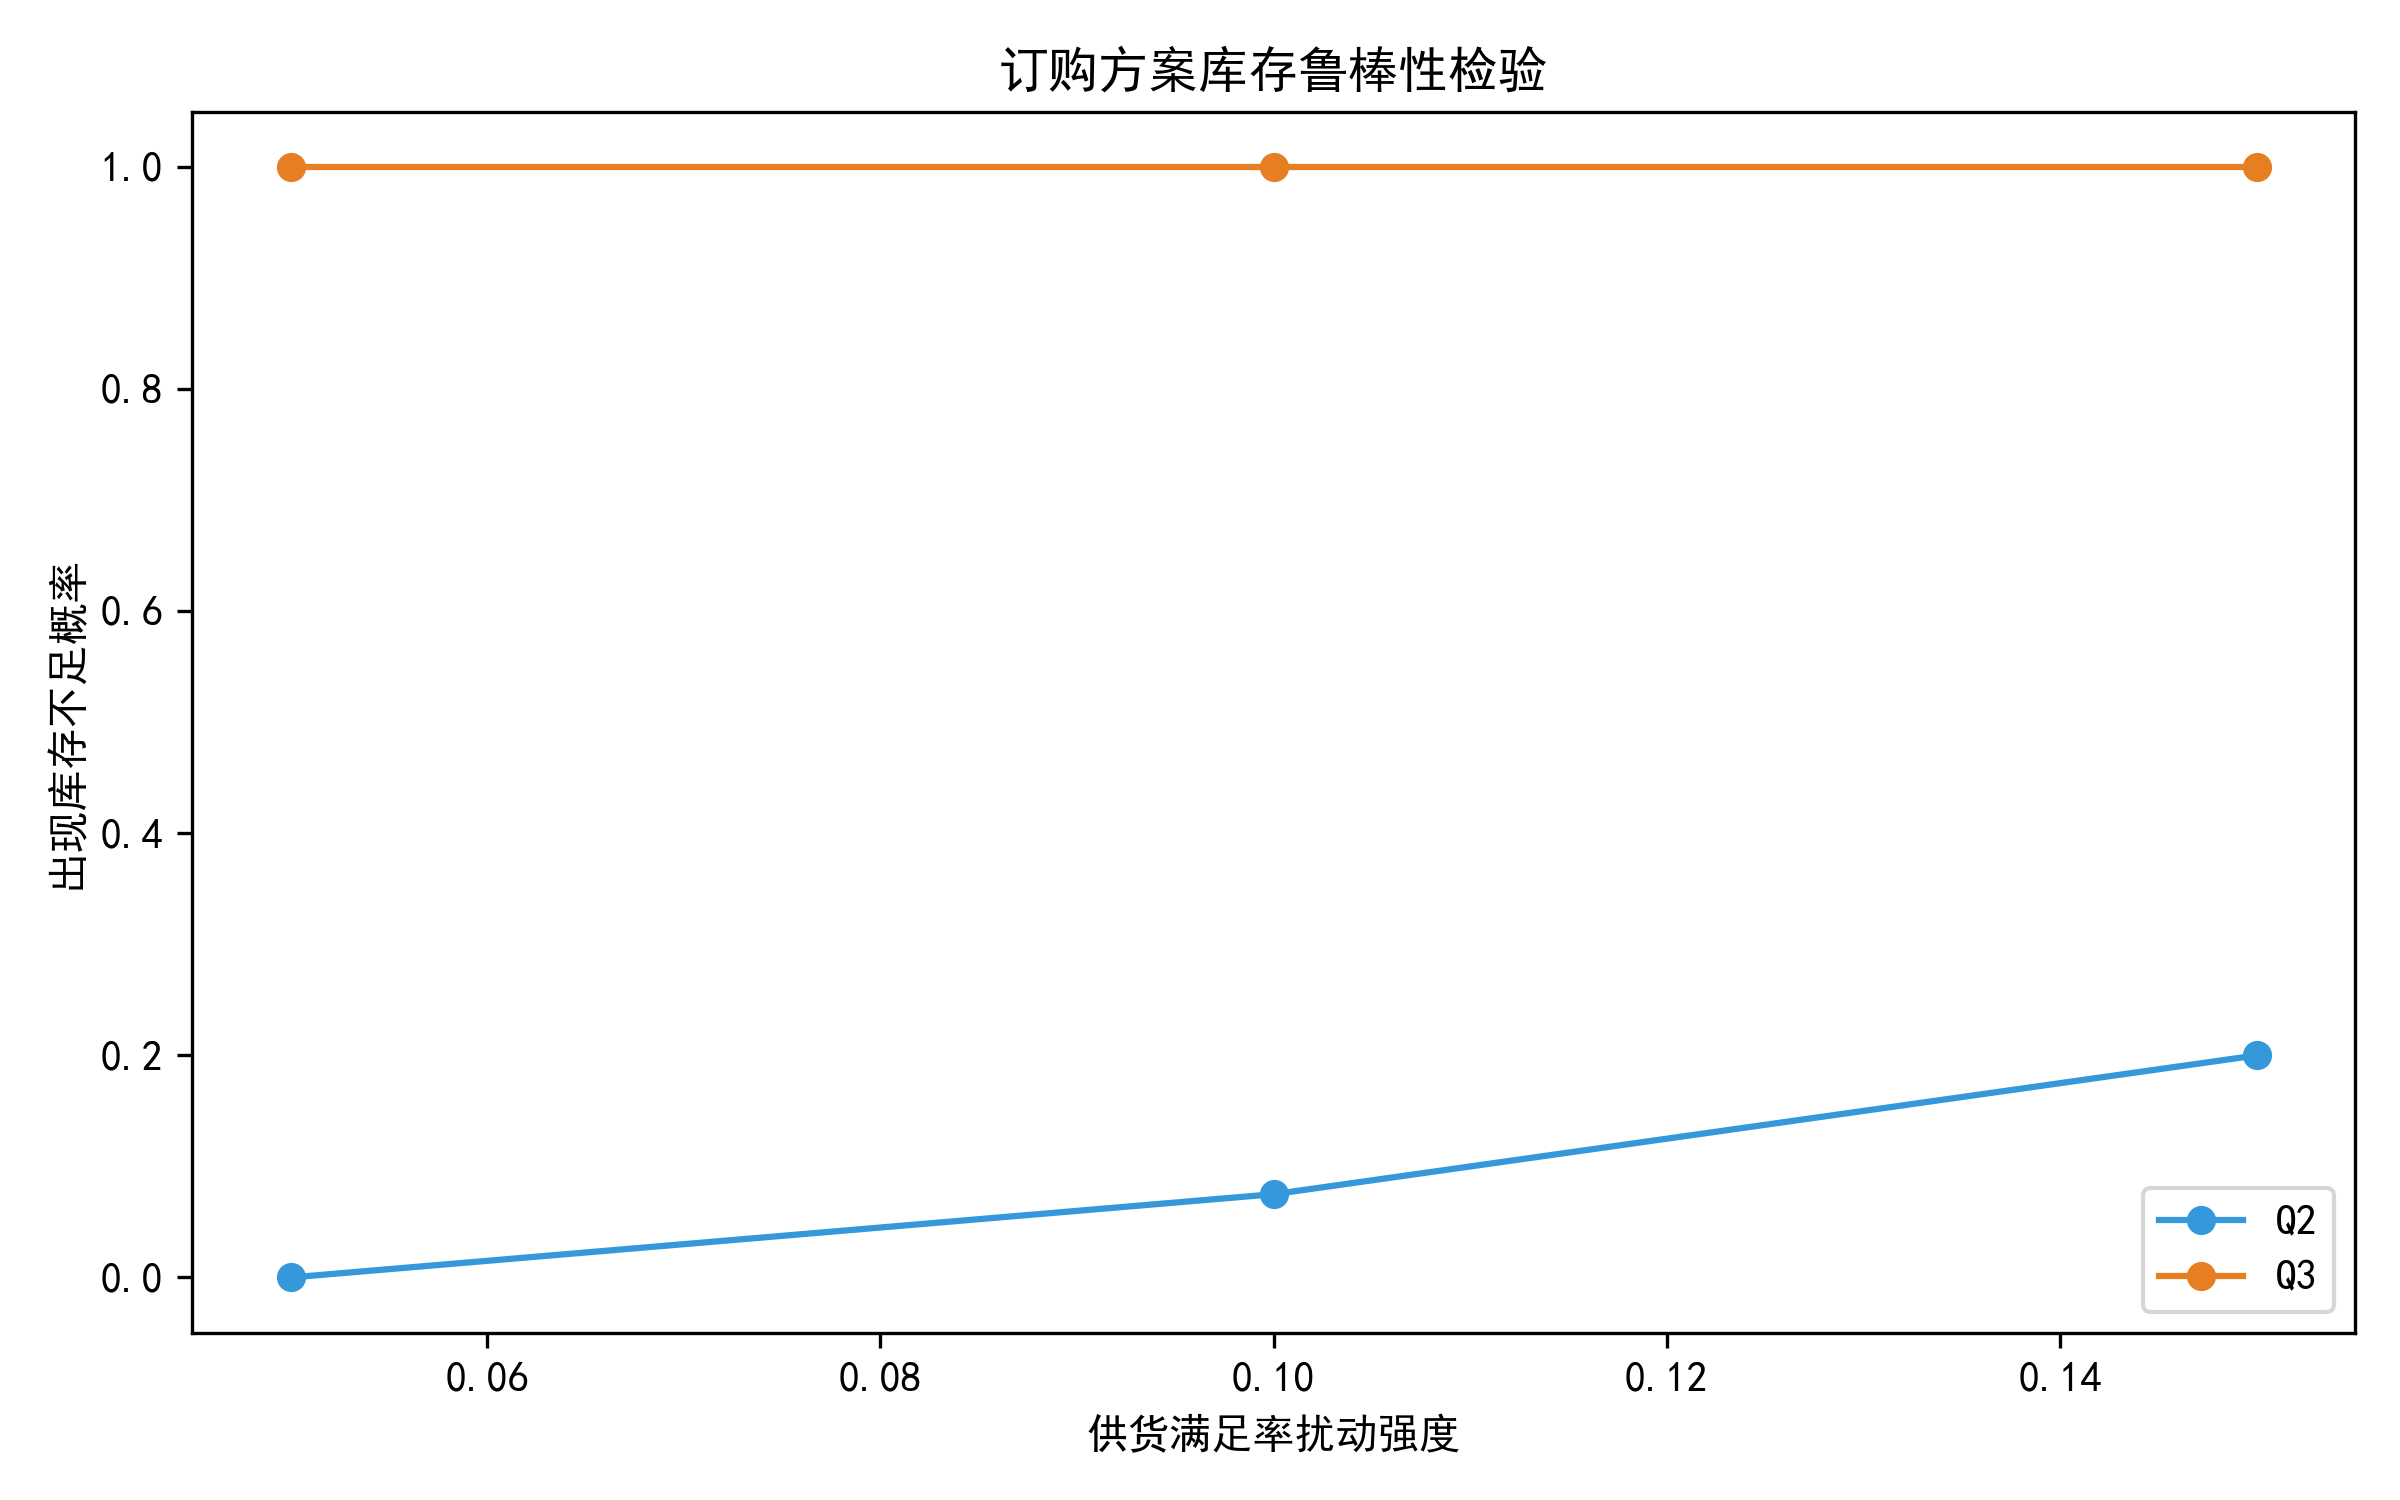
\includegraphics[width=0.75\textwidth]{../output/figures/robustness_inventory.png}
\caption{订购方案库存鲁棒性曲线}
\label{fig:rob}
\end{figure}


\section{模型的创新点、评价与推广}

\subsection{创新点（可验证）}
\begin{enumerate}[leftmargin=2em]
\item \textbf{生产保障导向的多维重要性测度 + 多方法交叉验证}：相对单一累计供货基准，融合履约与稳定性；CRITIC/灰关联/PCA对照与Kendall相关、Top50重叠提供可重复证据。
\item \textbf{产品当量统一库存约束的订购—转运两阶段框架}：将A/B/C消耗差异纳入同一LP，Q2/Q3/Q4共用内核，仅切换目标与筛选规则，保证逻辑贯通。
\item \textbf{结构偏好的可解释优化}：用“优先级重排+体积机制”落实多A少C，并用产品当量表量化实施效果，避免拍脑袋配比。
\item \textbf{双瓶颈产能上界与系统检验闭环}：供应能力与转运运力联合约束；配套权重灵敏度、价格灵敏度、蒙特卡洛评价鲁棒与库存鲁棒，形成“建模—求解—检验”闭环。
\end{enumerate}

\subsection{优点与不足}
\textbf{优点：}数据驱动、符号一致、结果可复现（\texttt{python run\_all.py}）；输出符合附件A/B格式；检验充分。\\
\textbf{不足：}供货不确定性未建完全随机规划；转运层以贪心为主，极端高峰周可能需MIP精细拆分；问题四高倍增方案动用供应商过多，实务需分阶段扩产。

\subsection{改进与推广}
可引入机会约束/CVaR控制缺货风险；将转运层升级为最小化$\sum X_{ikt}L_{kt}$的运输问题或整数规划；对接滚动时域（MPC）实现周度重计划；推广至多工厂、多仓库网络。

\section{结论}
本文完成了从供应商重要性识别，到最少供应商与经济订购—低损耗转运，再到结构优化与产能上界评估的完整闭环。主要定量结论：Top50由熵权-TOPSIS确定，Top1为S140；满足生产至少需14家供应商；Q3实现A升C降且成本指数降7.2\%；周产能最大约可提升150.0\%至70489\,m$^3$。灵敏度与鲁棒性检验支持方案在中等扰动下仍可用。

\begin{thebibliography}{99}
\bibitem{topsis} Hwang C. L., Yoon K. \emph{Multiple Attribute Decision Making: Methods and Applications}. Springer, 1981.
\bibitem{entropy} Shannon C. E. A mathematical theory of communication. \emph{Bell System Technical Journal}, 1948, 27: 379--423.
\bibitem{critic} Diakoulaki D., Mavrotas G., Papayannakis L. Determining objective weights in multiple criteria problems: The critic method. \emph{Computers \& Operations Research}, 1995, 22(7): 763--770.
\bibitem{grey} Deng J. L. Control problems of grey systems. \emph{Systems \& Control Letters}, 1982, 1(5): 288--294.
\bibitem{lp} Dantzig G. B. \emph{Linear Programming and Extensions}. Princeton University Press, 1963.
\bibitem{or} Hillier F. S., Lieberman G. J. \emph{Introduction to Operations Research}. McGraw-Hill, 2015.
\bibitem{sp} Birge J. R., Louveaux F. \emph{Introduction to Stochastic Programming}. Springer, 2011.
\bibitem{mcdm} 徐泽水. 多属性决策理论与方法. 北京: 科学出版社, 2012.
\bibitem{scm} Chopra S., Meindl P. \emph{Supply Chain Management}. Pearson, 2016.
\bibitem{inv} Zipkin P. H. \emph{Foundations of Inventory Management}. McGraw-Hill, 2000.
\end{thebibliography}

\appendix
\section{50家最重要供应商完整名单}
\begin{longtable}{clccrrr}
\caption{50家最重要供应商完整名单}\\
\label{tab:top50full}\\
\toprule
排名 & ID & 材料 & 重要性得分 & 累计供货(m$^3$) & 周均供货 & 满足率 \\
\midrule
\endfirsthead
\toprule
排名 & ID & 材料 & 重要性得分 & 累计供货(m$^3$) & 周均供货 & 满足率 \\
\midrule
\endhead
\bottomrule
\endfoot
1 & S140 & B & 0.5991 & 302047 & 1379.2 & 1.200 \\
2 & S201 & A & 0.5614 & 81989 & 2928.2 & 0.536 \\
3 & S374 & C & 0.4963 & 49224 & 205.1 & 1.312 \\
4 & S229 & A & 0.4912 & 354887 & 1478.7 & 0.994 \\
5 & S348 & A & 0.4649 & 92421 & 476.4 & 1.070 \\
6 & S361 & C & 0.4599 & 328080 & 1367.0 & 0.992 \\
7 & S151 & C & 0.4335 & 194498 & 810.4 & 0.983 \\
8 & S108 & B & 0.3933 & 240950 & 1004.0 & 0.984 \\
9 & S139 & B & 0.3137 & 151862 & 684.1 & 1.244 \\
10 & S340 & B & 0.2800 & 171426 & 714.3 & 0.999 \\
11 & S282 & A & 0.2770 & 169340 & 705.6 & 1.013 \\
12 & S275 & A & 0.2576 & 158553 & 660.6 & 1.003 \\
13 & S126 & C & 0.2483 & 47540 & 522.4 & 0.990 \\
14 & S329 & A & 0.2462 & 156518 & 652.2 & 1.002 \\
15 & S330 & B & 0.2432 & 136652 & 569.4 & 0.986 \\
16 & S131 & B & 0.2291 & 137512 & 573.0 & 0.997 \\
17 & S308 & B & 0.2289 & 136998 & 570.8 & 0.975 \\
18 & S356 & C & 0.2267 & 130307 & 542.9 & 1.003 \\
19 & S395 & A & 0.2265 & 75843 & 1024.9 & 0.918 \\
20 & S307 & A & 0.2172 & 78196 & 457.3 & 1.244 \\
21 & S268 & C & 0.2069 & 129786 & 540.8 & 1.004 \\
22 & S306 & C & 0.1969 & 126096 & 525.4 & 1.005 \\
23 & S352 & A & 0.1696 & 89031 & 371.0 & 1.002 \\
24 & S194 & C & 0.1635 & 101365 & 422.4 & 1.002 \\
25 & S143 & A & 0.1358 & 82787 & 344.9 & 1.004 \\
26 & S037 & C & 0.1165 & 50686 & 322.8 & 1.150 \\
27 & S247 & C & 0.0962 & 56698 & 236.2 & 1.014 \\
28 & S284 & C & 0.0796 & 46597 & 194.2 & 1.038 \\
29 & S365 & C & 0.0737 & 41631 & 173.5 & 1.022 \\
30 & S031 & B & 0.0722 & 41207 & 171.7 & 1.020 \\
31 & S338 & B & 0.0693 & 30109 & 147.6 & 1.264 \\
32 & S040 & B & 0.0584 & 31905 & 132.9 & 1.019 \\
33 & S364 & B & 0.0545 & 28763 & 119.8 & 1.039 \\
34 & S055 & B & 0.0504 & 24041 & 100.2 & 1.040 \\
35 & S367 & B & 0.0504 & 26335 & 109.7 & 1.031 \\
36 & S346 & B & 0.0462 & 23240 & 96.8 & 1.016 \\
37 & S086 & C & 0.0445 & 17949 & 87.1 & 1.195 \\
38 & S210 & C & 0.0439 & 15694 & 133.0 & 0.832 \\
39 & S080 & C & 0.0409 & 19237 & 80.2 & 1.086 \\
40 & S294 & C & 0.0395 & 18842 & 78.5 & 1.042 \\
41 & S244 & C & 0.0373 & 16406 & 68.4 & 1.071 \\
42 & S218 & C & 0.0359 & 15483 & 64.5 & 1.098 \\
43 & S154 & A & 0.0356 & 7634 & 99.1 & 0.803 \\
44 & S273 & A & 0.0343 & 9484 & 105.4 & 0.993 \\
45 & S114 & A & 0.0313 & 10931 & 47.7 & 1.168 \\
46 & S074 & C & 0.0310 & 13051 & 76.3 & 1.006 \\
47 & S291 & A & 0.0292 & 7984 & 36.5 & 1.149 \\
48 & S003 & C & 0.0278 & 13138 & 68.8 & 1.060 \\
49 & S007 & A & 0.0274 & 6948 & 28.9 & 1.290 \\
50 & S123 & A & 0.0269 & 6449 & 26.9 & 1.138 \\
\end{longtable}

\section{核心算法与复现说明}
全部代码位于\texttt{code/}，一键复现：
\begin{verbatim}
pip install -r requirements.txt
python run_all.py
\end{verbatim}
主要模块：\texttt{01\_eda\_preprocess.py}（EDA）、\texttt{q1\_supplier\_importance.py}（评价）、
\texttt{optimization.py}（LP与转运）、\texttt{q2/q3/q4\_*.py}（分问求解）、
\texttt{05\_advanced\_analysis.py}（多方法对比、蒙特卡洛、鲁棒性）。数值结果见\texttt{output/tables/}，
订购/转运方案见\texttt{data/processed/}中附件A/B导出文件。

\section{补充说明}
（1）满足率定义为有订货周上$S_{it}/O_{it}$的均值；无订货周不计入。\\
（2）产品当量库存使混料生产下的“两周库存”约束具有可加性。\\
（3）问题三C类降至0是优化在“少C”方向上的端点解，论文已解释其体积机制；若业务需保留最低C份额，可增加$\sum_{m(i)=C}Q_{it}\ge Q_C^{\min}$软约束而不改变整体框架。

\end{document}
